% Mathematical and graphical reference: ../1-practice_activities/G11_T2_L1_C3_practice.tex
% User scope: retain the existing three independent exercises; exactly two tasks per problem.
\makeatletter
\def\input@path{{../../../preamble/}}
\makeatother
\input{preamble.tex}
% Shared renderer and semantic roles; no earlier content uses these markers.
\input{highlights/highlights.tex}
% \GTenHighlightsfalse % Uncomment to disable instructional highlights.
\HighlightRegistryPalette
\HighlightRegistryRoles
\usepackage{pdflscape}
\usepackage{needspace}

\geometry{letterpaper,margin=0.25in}
\pagestyle{empty}
\linespread{1.04}
\setlength{\parskip}{2pt}
\raggedbottom
% Structural styles for the printable activity only; no semantic highlighting.
\newcommand{\stageheading}[1]{%
    \par\Needspace{4\baselineskip}\addvspace{4pt}%
    {\centering\large\bfseries
     \tikz[baseline=(title.base)]{%
         \node[fill=black!10,text=black,rounded corners=2mm,
             inner sep=3pt,outer sep=0pt] (title) {\strut #1};}\par}%
    \nopagebreak[4]\smallskip
}
\newcommand{\criterionbox}[2]{%
    \begin{tcolorbox}[colback=white,colframe=black!45,boxrule=.4pt,
        arc=2mm,boxsep=0pt,left=6pt,right=6pt,top=5pt,bottom=5pt,
        before skip=4pt,after skip=4pt,width=\linewidth]
        \textbf{#1} #2
    \end{tcolorbox}%
}
\newcommand{\problemtitle}[2]{\par\textbf{#1. #2}\par}
\newcommand{\task}[2]{\par\textbf{#1} #2\par}
\newenvironment{datagrid}[1]{\par\begingroup\small\setlength{\tabcolsep}{4pt}\setlength{\parskip}{0pt}\renewcommand{\arraystretch}{1.03}\tabularx{\linewidth}{#1}\hline}{\endtabularx\par\endgroup}
\pgfplotsset{relation/.style={width=.94\linewidth,height=7.1cm,axis lines=left,
 grid=major,major grid style={black!15},tick label style={font=\small},
 label style={font=\small},scaled ticks=false,enlargelimits=false,clip=true,
 tick label style={/pgf/number format/1000 sep={}}}}
% Reference label format, ordinary grayscale typography, five IDs per graph.
\newcommand{\PointLabel}[7]{%
 \node[font=\small,fill=white,inner sep=1.5pt,anchor=#7] (point#1)
 at (axis description cs:#5,#6) {#1: $(#3,\,#4)$};
 \draw[black!70,line width=.35pt,shorten <=2.5pt] (axis cs:#2)--(point#1);
}
% Scoped to the two linear worked-example panels: equally spaced west
% anchors on y=slope*x+offset, parallel to the normalized data line.
\newcommand{\LinearGuideLabel}[6][south east]{%
 \pgfmathsetmacro{\guideX}{\guideStart+#6*\guideStep}%
 \pgfmathsetmacro{\guideY}{\guideSlope*\guideX+\guideOffset}%
 % Freeze coordinates before pgfplots defers axis-node placement.
 \edef\placeGuide{\noexpand\coordinate (guide#2) at
 (axis description cs:\guideX,\guideY);}\placeGuide
 \node[font=\small,fill=white,inner sep=1pt,anchor=west] (point#2)
 at (guide#2) {#2: $(#4,\,#5)$};
 \draw[black!70,line width=.35pt,shorten <=2.5pt]
 (axis cs:#3)--(point#2.#1);
}
\newcommand{\LabelTemplates}{%
 \node[anchor=east,font=\small,fill=white,inner sep=1.5pt] at (axis description cs:.97,.93) {A: $(\underline{\hspace{.65cm}},\,\underline{\hspace{.65cm}})$};
 \node[anchor=east,font=\small,fill=white,inner sep=1.5pt] at (axis description cs:.97,.83) {B: $(\underline{\hspace{.65cm}},\,\underline{\hspace{.65cm}})$};
 \node[anchor=east,font=\small,fill=white,inner sep=1.5pt] at (axis description cs:.97,.73) {C: $(\underline{\hspace{.65cm}},\,\underline{\hspace{.65cm}})$};
 \node[anchor=east,font=\small,fill=white,inner sep=1.5pt] at (axis description cs:.97,.63) {D: $(\underline{\hspace{.65cm}},\,\underline{\hspace{.65cm}})$};
 \node[anchor=east,font=\small,fill=white,inner sep=1.5pt] at (axis description cs:.97,.53) {E: $(\underline{\hspace{.65cm}},\,\underline{\hspace{.65cm}})$};}
\newcommand{\workarea}{\begin{minipage}[t]{.49\linewidth}\vspace{0pt}
 \textbf{Calculation workspace}\par\smallskip
 \begin{tikzpicture}\draw[black!40] (0,0) rectangle (9.65,5.6);\end{tikzpicture}
 \end{minipage}}
\newcommand{\normalpanel}[2]{%
 \par\noindent\begin{tikzpicture}\begin{axis}[
 width=.80\linewidth,height=1.05cm,scale only axis,
 xmin=-4,xmax=4,ymin=0,ymax=.46,enlargelimits=false,axis lines=left,
 xtick={-#2,0,#2},xticklabels={$-#2$,0,$+#2$},ytick={0,.4},
 tick label style={font=\footnotesize},label style={font=\small},
 title={$C=#1\%\qquad -z^*=-#2,\quad +z^*=+#2$},
 title style={font=\small,yshift=-2pt}]
 \addplot[draw=none,fill=black!18,domain=-#2:#2,samples=161]
 {exp(-x*x/2)/sqrt(2*pi)}\closedcycle;
 \addplot[black,thick,domain=-4:4,samples=201] {exp(-x*x/2)/sqrt(2*pi)};
 \draw[dashed] (axis cs:-#2,0)--(axis cs:-#2,.33)
 (axis cs:#2,0)--(axis cs:#2,.33);
 \node[font=\small] at (axis cs:0,.17) {$#1\%$};
 \end{axis}\end{tikzpicture}\par}
\begin{document}
{\centering{\Large\bfseries C3: Anatomy of a confidence interval\par}
Global Economics | Grade 11 | Term 2 | Lesson 1\par}
\criterionbox{C3}{Identifies the components of a confidence interval, including point estimate, critical value, standard error, and margin of error, explaining how each component affects precision and reliability.}


\stageheading{Equations and basic procedure}
A confidence interval estimates an unknown population mean $\mu$ and shows the uncertainty around a sample mean. Its width depends on population variability, sample size, and confidence.\par
\begingroup
\small\setlength{\tabcolsep}{3pt}\setlength{\extrarowheight}{0pt}
\setlength{\parskip}{0pt}\renewcommand{\arraystretch}{1}
\begin{tabularx}{\linewidth}{@{}>{\raggedright\arraybackslash}p{.12\linewidth}>{\raggedright\arraybackslash}p{.23\linewidth}>{\raggedright\arraybackslash}X@{}}
\toprule
\textbf{Symbol} & \textbf{Concept} & \textbf{Definition and formula}\\\midrule
$\mathrm{CI}$ & Confidence interval & Range estimating $\mu$: $[\bar{x}-\mathrm{MoE},\bar{x}+\mathrm{MoE}]$; in the measured units.\\
$\bar{x}$ & Point estimate & Sample mean estimating $\mu$; centre of the interval, in the measured units.\\
$C$ & Confidence level & Nominal long-run percentage of intervals covering $\mu$ under the model.\\
$z^*$ & Critical value & Positive standard normal cutoff with central area $C/100$ when $C$ is a percentage; unitless.\\
$\mathrm{SE}$ & Standard error & Standard deviation of sample means: $\mathrm{SE}=\sigma/\sqrt n$; in the measured units.\\
$\mathrm{MoE}$ & Margin of error & Distance from the estimate to either endpoint: $\mathrm{MoE}=z^*\mathrm{SE}$; in the measured units.\\
$\sigma$ & Population standard deviation & Known spread of individual population values; in the measured units.\\
$n$ & Sample size & Number of sampled units; a positive integer count.\\
\bottomrule
\end{tabularx}\par\endgroup

\stageheading{General tasks}
\task{Task 1 -- Investigate SE, MoE, and sample size with $\mathbf{\sigma}$ and confidence fixed.}{}
Calculate SE and MoE for the five sample sizes, assigned A--E in the stated order. Draw (top left) SE vs $n$, (top right) MoE vs $n$, and (bottom left) MoE vs SE. 

\task{Task 2 -- Investigate confidence, critical value, and MoE with $n$ and $\sigma$ fixed.}{}
Calculate the fixed SE and the MoE for each supplied $(C,z^*)$ pair. Draw (top left) confidence vs MoE, (top right) critical value vs MoE, and (bottom left) confidence vs critical value. Use these five cases in every problem:
\begin{datagrid}{|l|X|X|X|X|X|}ID&A&B&C&D&E\\\hline
$C$ (\%)&80&90&95&99&99.9\\\hline
$z^*$&1.282&1.645&1.960&2.576&3.291\\\hline\end{datagrid}

\vspace{2mm}
\textbf{For both tasks.} Plot all five cases in each relationship graph, label A--E with their $(x,y)$ coordinates, and draw the corresponding curve or line. SE and MoE have the context's monetary units; $n$ counts sampled units, $C$ uses percent, and $z^*$ is unitless. The bottom-right cell is calculation workspace in student problems; supplementary illustrations appear only in the worked example.

\pgfplotsset{relation/.append style={height=5.5cm}}
\stageheading{Worked example}
\problemtitle{1}{Weekly household grocery spending} 
An analyst estimates the district mean weekly household grocery bill. For the explanatory intervals, the common point estimate is $\bar{x}=84$ thousand COP.
Population SD is known: $\sigma=30$ thousand COP; the common assumptions apply. For Task 1, fix $C=95\%$ ($z^*=1.960$) and use $n=25,100,400,900,1600$ for A--E, respectively. For Task 2, fix $n=100$ and the same $\sigma$, using the five general $(C,z^*)$ cases.
\task{Task 1 -- Investigate SE, MoE, and sample size with $\mathbf{\sigma}$ and confidence fixed.}{}
\noindent\begin{minipage}[t]{.30\linewidth}\vspace{0pt}
\textbf{Solution.} For A, $\mathrm{SE}=30/\sqrt{25}=6.000$ and $\mathrm{MoE}=1.960(6.000)=11.760$ thousand COP. The remaining substitutions supply the other plotted coordinates.
\end{minipage}\hfill
\begin{minipage}[t]{.68\linewidth}\vspace{0pt}
\begin{datagrid}{|l|r|X|X|}ID&$n$&SE (thousand COP)&MoE (thousand COP)\\\hline
A&25&$30/\sqrt{25}=6.000$&$1.960(6.000)=11.760$\\\hline
B&100&$30/\sqrt{100}=3.000$&$1.960(3.000)=5.880$\\\hline
C&400&$30/\sqrt{400}=1.500$&$1.960(1.500)=2.940$\\\hline
D&900&$30/\sqrt{900}=1.000$&$1.960(1.000)=1.960$\\\hline
E&1600&$30/\sqrt{1600}=0.750$&$1.960(0.750)=1.470$\\\hline
\end{datagrid}
\end{minipage}\par
\par\smallskip
\begin{minipage}[t]{.49\linewidth}\vspace{0pt}\centering\textbf{Standard error vs sample size}\par\smallskip
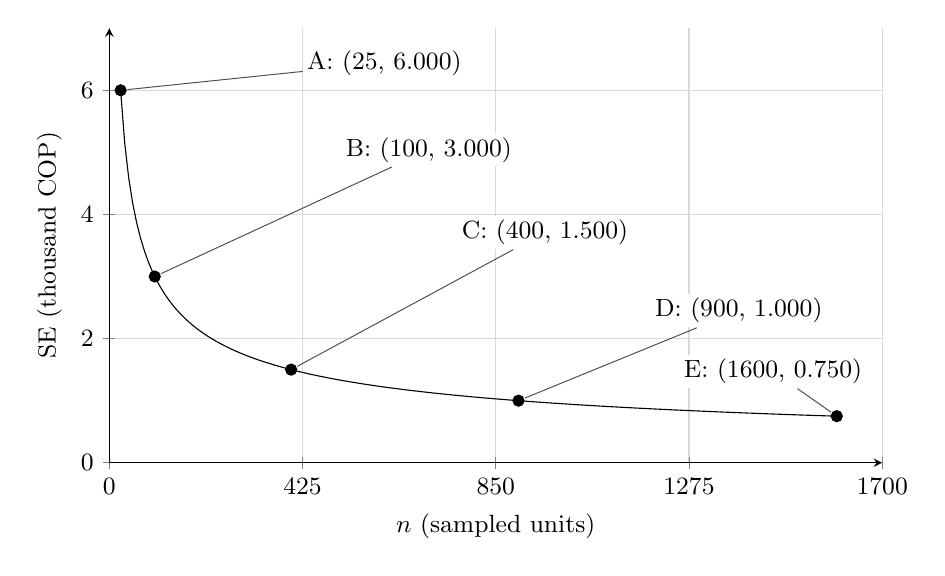
\begin{tikzpicture}\begin{axis}[relation,xlabel={$n$ (sampled units)},ylabel={SE (thousand COP)},xmin=0,xmax=1700,ymin=0,ymax=7,xtick={0,425,850,1275,1700}]
\addplot[black,domain=25:1600,samples=180] {30/sqrt(x)};
\addplot[only marks,mark=*,mark size=2pt] coordinates {(25.000000000,6.000000000) (100.000000000,3.000000000) (400.000000000,1.500000000) (900.000000000,1.000000000) (1600.000000000,0.750000000)};
\PointLabel{A}{25.000000000,6.000000000}{25}{6.000}{0.25}{0.92}{west}
\PointLabel{B}{100.000000000,3.000000000}{100}{3.000}{0.3}{0.72}{west}
\PointLabel{C}{400.000000000,1.500000000}{400}{1.500}{0.45}{0.53}{west}
\PointLabel{D}{900.000000000,1.000000000}{900}{1.000}{0.7}{0.35}{west}
\PointLabel{E}{1600.000000000,0.750000000}{1600}{0.750}{0.98}{0.21}{east}
\end{axis}\end{tikzpicture}\end{minipage}
\hfill
\begin{minipage}[t]{.49\linewidth}\vspace{0pt}\centering\textbf{Margin of error vs sample size}\par\smallskip
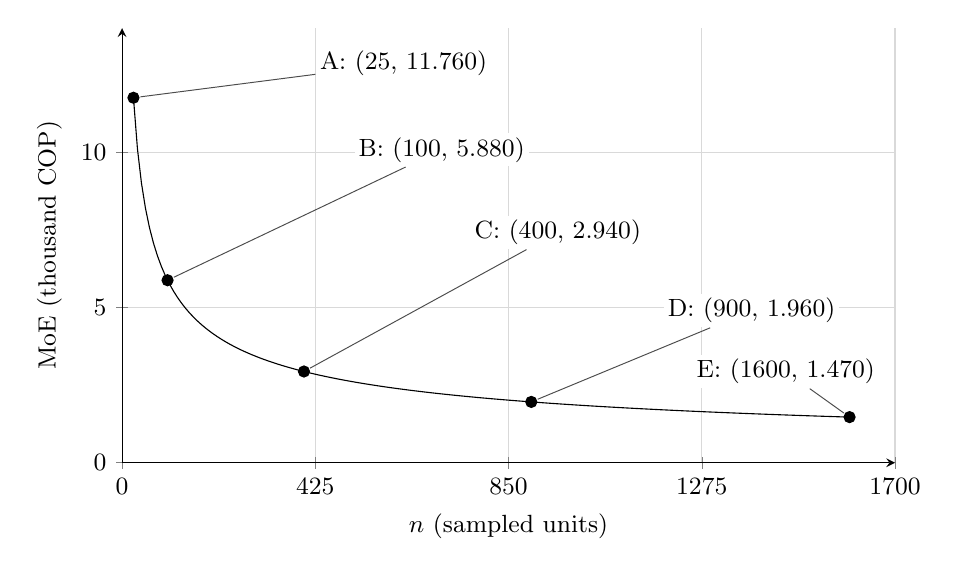
\begin{tikzpicture}\begin{axis}[relation,xlabel={$n$ (sampled units)},ylabel={MoE (thousand COP)},xmin=0,xmax=1700,ymin=0,ymax=14,xtick={0,425,850,1275,1700}]
\addplot[black,domain=25:1600,samples=180] {1.960*30/sqrt(x)};
\addplot[only marks,mark=*,mark size=2pt] coordinates {(25.000000000,11.760000000) (100.000000000,5.880000000) (400.000000000,2.940000000) (900.000000000,1.960000000) (1600.000000000,1.470000000)};
\PointLabel{A}{25.000000000,11.760000000}{25}{11.760}{0.25}{0.92}{west}
\PointLabel{B}{100.000000000,5.880000000}{100}{5.880}{0.3}{0.72}{west}
\PointLabel{C}{400.000000000,2.940000000}{400}{2.940}{0.45}{0.53}{west}
\PointLabel{D}{900.000000000,1.960000000}{900}{1.960}{0.7}{0.35}{west}
\PointLabel{E}{1600.000000000,1.470000000}{1600}{1.470}{0.98}{0.21}{east}
\end{axis}\end{tikzpicture}\end{minipage}
\par\medskip
\begin{minipage}[t]{.49\linewidth}\vspace{0pt}\centering\textbf{Margin of error vs standard error}\par\smallskip
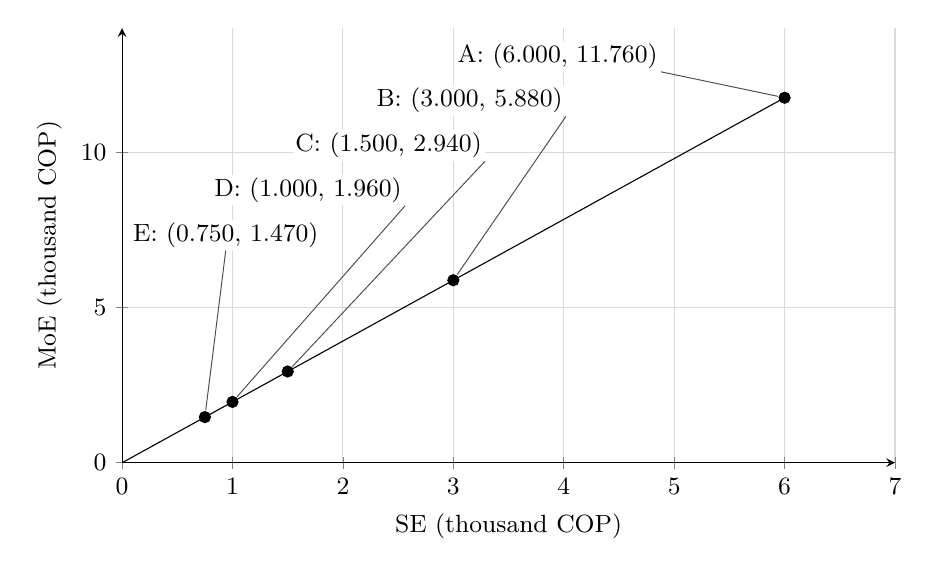
\begin{tikzpicture}\begin{axis}[relation,xlabel={SE (thousand COP)},ylabel={MoE (thousand COP)},xmin=0,xmax=7,ymin=0,ymax=14]
\addplot[black,domain=0:6.0] {1.960*x};
\addplot[only marks,mark=*,mark size=2pt] coordinates {(6.000000000,11.760000000) (3.000000000,5.880000000) (1.500000000,2.940000000) (1.000000000,1.960000000) (0.750000000,1.470000000)};
\def\guideStart{0.010}\def\guideStep{0.105}%
\def\guideSlope{1.960*7/14}\def\guideOffset{0.5147}%
\LinearGuideLabel{A}{6.000000000,11.760000000}{6.000}{11.760}{4}
\LinearGuideLabel{B}{3.000000000,5.880000000}{3.000}{5.880}{3}
\LinearGuideLabel{C}{1.500000000,2.940000000}{1.500}{2.940}{2}
\LinearGuideLabel[south east]{D}{1.000000000,1.960000000}{1.000}{1.960}{1}
\LinearGuideLabel[south]{E}{0.750000000,1.470000000}{0.750}{1.470}{0}
\end{axis}\end{tikzpicture}

SE $\sim$ MoE $\sim$ $1/\sqrt n$. Larger samples give narrower intervals and greater precision at the same 95\% confidence.

\end{minipage}
\hfill\begin{minipage}[t]{.49\linewidth}\vspace{0pt}\small
\textbf{Explanatory confidence-interval comparison}\par
These three intervals use $\bar{x}\pm\mathrm{MoE}=84\pm1.960(30/\sqrt n)$, in 1000 COP:\par
\(\begin{gathered}
\begin{aligned}
n=25:&\quad84\pm11.760=[72.240,95.760],\\
n=400:&\quad84\pm2.940=[81.060,86.940],\\
n=1600:&\quad84\pm1.470=[82.530,85.470].
\end{aligned}
\end{gathered}\)
\centering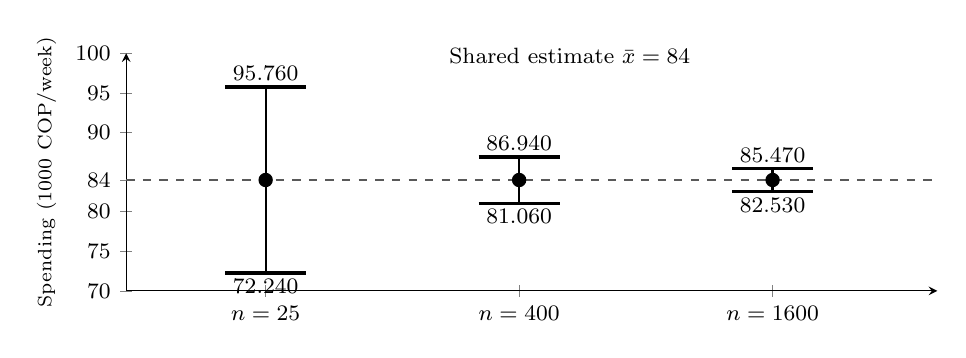
\begin{tikzpicture}\begin{axis}[
width=.98\linewidth,height=4.6cm,xmin=.45,xmax=3.65,ymin=70,ymax=100,
axis x line=bottom,axis y line=left,xtick={1,2,3},
xticklabels={$n=25$,$n=400$,$n=1600$},ytick={70,75,80,84,90,95,100},
tick label style={font=\footnotesize},label style={font=\footnotesize},
ylabel={\scriptsize Spending (1000 COP/week)},scaled ticks=false,clip=false]
\draw[dashed,black!65] (axis cs:.45,84)--(axis cs:3.65,84);
\node[font=\footnotesize,anchor=south] at (axis cs:2.2,97.5) {Shared estimate $\bar{x}=84$};
\draw[thick] (axis cs:1,72.240)--(axis cs:1,95.760);
\draw[line width=1.3pt] (axis cs:0.84,72.240)--(axis cs:1.16,72.240)
(axis cs:0.84,95.760)--(axis cs:1.16,95.760);
\fill (axis cs:1,84) circle (2.6pt);
\node[font=\footnotesize,anchor=north,inner sep=2pt] at (axis cs:1,72.240) {72.240};
\node[font=\footnotesize,anchor=south,inner sep=2pt] at (axis cs:1,95.760) {95.760};
\draw[thick] (axis cs:2,81.060)--(axis cs:2,86.940);
\draw[line width=1.3pt] (axis cs:1.84,81.060)--(axis cs:2.16,81.060)
(axis cs:1.84,86.940)--(axis cs:2.16,86.940);
\fill (axis cs:2,84) circle (2.6pt);
\node[font=\footnotesize,anchor=north,inner sep=2pt] at (axis cs:2,81.060) {81.060};
\node[font=\footnotesize,anchor=south,inner sep=2pt] at (axis cs:2,86.940) {86.940};
\draw[thick] (axis cs:3,82.530)--(axis cs:3,85.470);
\draw[line width=1.3pt] (axis cs:2.84,82.530)--(axis cs:3.16,82.530)
(axis cs:2.84,85.470)--(axis cs:3.16,85.470);
\fill (axis cs:3,84) circle (2.6pt);
\node[font=\footnotesize,anchor=north,inner sep=2pt] at (axis cs:3,82.530) {82.530};
\node[font=\footnotesize,anchor=south,inner sep=2pt] at (axis cs:3,85.470) {85.470};
\end{axis}\end{tikzpicture}\par
\end{minipage}\par

\vspace{4mm}

\task{Task 2  -- Investigate confidence, critical value, and MoE with $n$ and $\sigma$ fixed.}{Use $n=100$}
\textbf{Solution.} $\mathrm{SE}=30/\sqrt{100}=3.000$ thousand COP. Thus the five margins are $1.282(3)=3.846$, $1.645(3)=4.935$, $1.960(3)=5.880$, $2.576(3)=7.728$ and $3.291(3)=9.873$ thousand COP.
\par\smallskip
\begin{minipage}[t]{.49\linewidth}\vspace{0pt}\centering\textbf{Confidence level vs margin of error}\par\smallskip
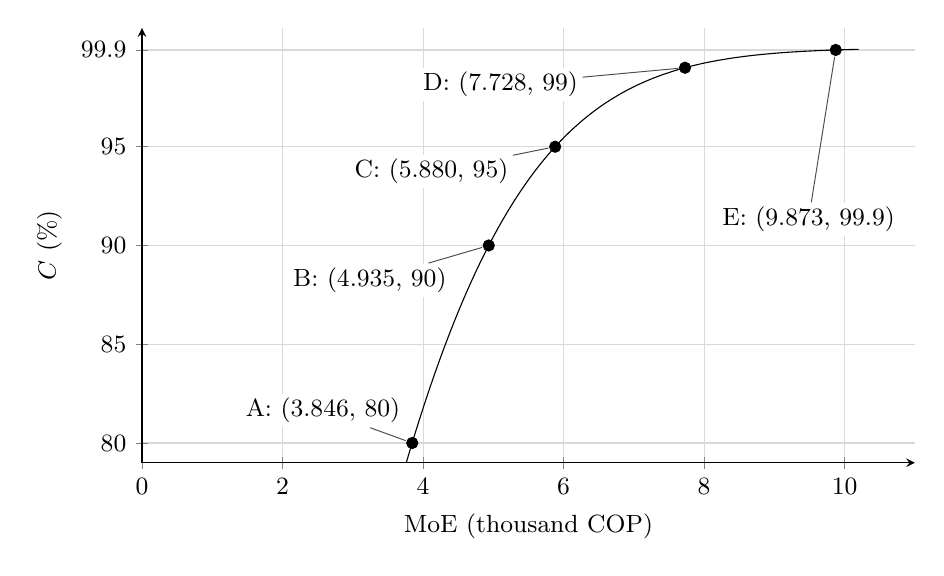
\begin{tikzpicture}\begin{axis}[relation,xlabel={MoE (thousand COP)},ylabel={$C$ (\%)},xmin=0,xmax=11,ymin=79,ymax=101,ytick={80,85,90,95,99.9}]
\addplot[black] coordinates {(3.600000000,76.986065956) (3.636666667,77.457267281) (3.673333333,77.921538814) (3.710000000,78.378914140) (3.746666667,78.829428390) (3.783333333,79.273118204) (3.820000000,79.710021689) (3.856666667,80.140178381) (3.893333333,80.563629207) (3.930000000,80.980416441) (3.966666667,81.390583669) (4.003333333,81.794175746) (4.040000000,82.191238757) (4.076666667,82.581819974) (4.113333333,82.965967820) (4.150000000,83.343731826) (4.186666667,83.715162592) (4.223333333,84.080311743) (4.260000000,84.439231895) (4.296666667,84.791976609) (4.333333333,85.138600354) (4.370000000,85.479158469) (4.406666667,85.813707116) (4.443333333,86.142303250) (4.480000000,86.465004571) (4.516666667,86.781869494) (4.553333333,87.092957100) (4.590000000,87.398327107) (4.626666667,87.698039826) (4.663333333,87.992156125) (4.700000000,88.280737392) (4.736666667,88.563845498) (4.773333333,88.841542760) (4.810000000,89.113891904) (4.846666667,89.380956033) (4.883333333,89.642798585) (4.920000000,89.899483305) (4.956666667,90.151074208) (4.993333333,90.397635545) (5.030000000,90.639231769) (5.066666667,90.875927504) (5.103333333,91.107787513) (5.140000000,91.334876665) (5.176666667,91.557259905) (5.213333333,91.775002224) (5.250000000,91.988168627) (5.286666667,92.196824108) (5.323333333,92.401033617) (5.360000000,92.600862035) (5.396666667,92.796374145) (5.433333333,92.987634608) (5.470000000,93.174707932) (5.506666667,93.357658453) (5.543333333,93.536550307) (5.580000000,93.711447404) (5.616666667,93.882413408) (5.653333333,94.049511715) (5.690000000,94.212805427) (5.726666667,94.372357332) (5.763333333,94.528229888) (5.800000000,94.680485196) (5.836666667,94.829184985) (5.873333333,94.974390591) (5.910000000,95.116162944) (5.946666667,95.254562542) (5.983333333,95.389649443) (6.020000000,95.521483244) (6.056666667,95.650123066) (6.093333333,95.775627542) (6.130000000,95.898054799) (6.166666667,96.017462450) (6.203333333,96.133907575) (6.240000000,96.247446713) (6.276666667,96.358135850) (6.313333333,96.466030405) (6.350000000,96.571185226) (6.386666667,96.673654573) (6.423333333,96.773492113) (6.460000000,96.870750912) (6.496666667,96.965483425) (6.533333333,97.057741490) (6.570000000,97.147576318) (6.606666667,97.235038493) (6.643333333,97.320177959) (6.680000000,97.403044022) (6.716666667,97.483685338) (6.753333333,97.562149914) (6.790000000,97.638485104) (6.826666667,97.712737601) (6.863333333,97.784953441) (6.900000000,97.855177996) (6.936666667,97.923455973) (6.973333333,97.989831414) (7.010000000,98.054347695) (7.046666667,98.117047523) (7.083333333,98.177972938) (7.120000000,98.237165314) (7.156666667,98.294665358) (7.193333333,98.350513110) (7.230000000,98.404747948) (7.266666667,98.457408586) (7.303333333,98.508533080) (7.340000000,98.558158826) (7.376666667,98.606322564) (7.413333333,98.653060386) (7.450000000,98.698407731) (7.486666667,98.742399394) (7.523333333,98.785069530) (7.560000000,98.826451657) (7.596666667,98.866578658) (7.633333333,98.905482789) (7.670000000,98.943195683) (7.706666667,98.979748356) (7.743333333,99.015171209) (7.780000000,99.049494036) (7.816666667,99.082746030) (7.853333333,99.114955789) (7.890000000,99.146151318) (7.926666667,99.176360042) (7.963333333,99.205608807) (8.000000000,99.233923886) (8.036666667,99.261330993) (8.073333333,99.287855279) (8.110000000,99.313521347) (8.146666667,99.338353257) (8.183333333,99.362374529) (8.220000000,99.385608156) (8.256666667,99.408076609) (8.293333333,99.429801841) (8.330000000,99.450805300) (8.366666667,99.471107932) (8.403333333,99.490730189) (8.440000000,99.509692041) (8.476666667,99.528012976) (8.513333333,99.545712013) (8.550000000,99.562807709) (8.586666667,99.579318164) (8.623333333,99.595261032) (8.660000000,99.610653524) (8.696666667,99.625512422) (8.733333333,99.639854079) (8.770000000,99.653694435) (8.806666667,99.667049015) (8.843333333,99.679932946) (8.880000000,99.692360958) (8.916666667,99.704347393) (8.953333333,99.715906214) (8.990000000,99.727051011) (9.026666667,99.737795010) (9.063333333,99.748151076) (9.100000000,99.758131727) (9.136666667,99.767749133) (9.173333333,99.777015132) (9.210000000,99.785941229) (9.246666667,99.794538609) (9.283333333,99.802818141) (9.320000000,99.810790383) (9.356666667,99.818465596) (9.393333333,99.825853741) (9.430000000,99.832964493) (9.466666667,99.839807245) (9.503333333,99.846391114) (9.540000000,99.852724948) (9.576666667,99.858817332) (9.613333333,99.864676596) (9.650000000,99.870310818) (9.686666667,99.875727832) (9.723333333,99.880935234) (9.760000000,99.885940387) (9.796666667,99.890750427) (9.833333333,99.895372271) (9.870000000,99.899812617) (9.906666667,99.904077957) (9.943333333,99.908174575) (9.980000000,99.912108558) (10.016666667,99.915885798) (10.053333333,99.919511999) (10.090000000,99.922992681) (10.126666667,99.926333183) (10.163333333,99.929538672) (10.200000000,99.932614147)};
\addplot[only marks,mark=*,mark size=2pt] coordinates {(3.846000000,80.000000000) (4.935000000,90.000000000) (5.880000000,95.000000000) (7.728000000,99.000000000) (9.873000000,99.900000000)};
\PointLabel{A}{3.846000000,80.000000000}{3.846}{80}{0.34}{0.12}{east}
\PointLabel{B}{4.935000000,90.000000000}{4.935}{90}{0.40}{0.42}{east}
\PointLabel{C}{5.880000000,95.000000000}{5.880}{95}{0.48}{0.67}{east}
\PointLabel{D}{7.728000000,99.000000000}{7.728}{99}{0.57}{0.87}{east}
\PointLabel{E}{9.873000000,99.900000000}{9.873}{99.9}{0.98}{0.56}{east}
\end{axis}\end{tikzpicture}\end{minipage}
\hfill
\begin{minipage}[t]{.49\linewidth}\vspace{0pt}\centering\textbf{Critical value vs margin of error}\par\smallskip
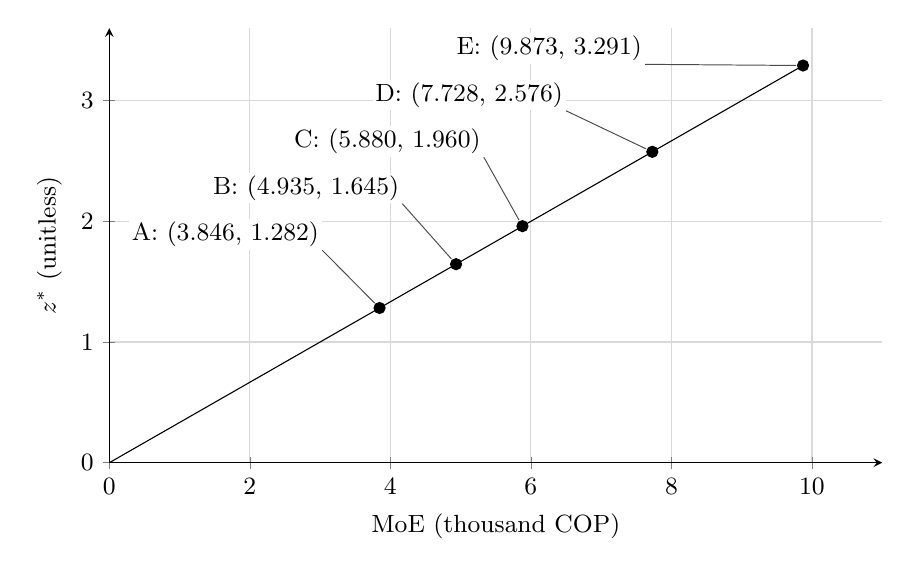
\begin{tikzpicture}\begin{axis}[relation,xlabel={MoE (thousand COP)},ylabel={$z^*$ (unitless)},xmin=0,xmax=11,ymin=0,ymax=3.6,ytick={0,1,2,3}]
\addplot[black,domain=0:9.873] {x/3.0};
\addplot[only marks,mark=*,mark size=2pt] coordinates {(3.846000000,1.282000000) (4.935000000,1.645000000) (5.880000000,1.960000000) (7.728000000,2.576000000) (9.873000000,3.291000000)};
\def\guideStart{0.025}\def\guideStep{0.105}%
\def\guideSlope{11/(3*3.6)}\def\guideOffset{0.50}%
\LinearGuideLabel{A}{3.846000000,1.282000000}{3.846}{1.282}{0}
\LinearGuideLabel{B}{4.935000000,1.645000000}{4.935}{1.645}{1}
\LinearGuideLabel{C}{5.880000000,1.960000000}{5.880}{1.960}{2}
\LinearGuideLabel{D}{7.728000000,2.576000000}{7.728}{2.576}{3}
\LinearGuideLabel{E}{9.873000000,3.291000000}{9.873}{3.291}{4}
\end{axis}\end{tikzpicture}\end{minipage}
\par\medskip
\begin{minipage}[t]{.49\linewidth}\vspace{0pt}\centering\textbf{Confidence level vs critical value}\par\smallskip
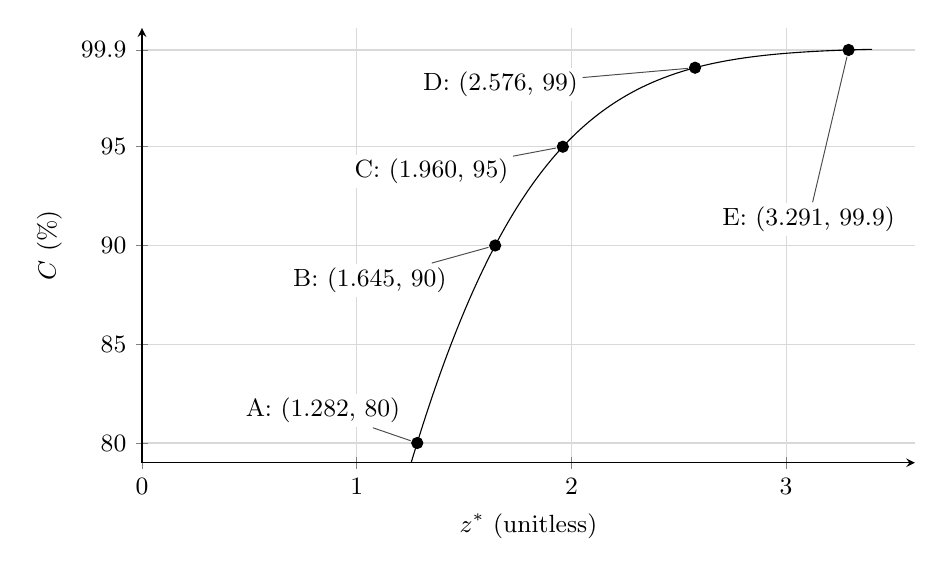
\begin{tikzpicture}\begin{axis}[relation,xlabel={$z^*$ (unitless)},ylabel={$C$ (\%)},xmin=0,xmax=3.6,ymin=79,ymax=101,xtick={0,1,2,3},ytick={80,85,90,95,99.9}]
\addplot[black] coordinates {(1.200000000,76.986065956) (1.212222222,77.457267281) (1.224444444,77.921538814) (1.236666667,78.378914140) (1.248888889,78.829428390) (1.261111111,79.273118204) (1.273333333,79.710021689) (1.285555556,80.140178381) (1.297777778,80.563629207) (1.310000000,80.980416441) (1.322222222,81.390583669) (1.334444444,81.794175746) (1.346666667,82.191238757) (1.358888889,82.581819974) (1.371111111,82.965967820) (1.383333333,83.343731826) (1.395555556,83.715162592) (1.407777778,84.080311743) (1.420000000,84.439231895) (1.432222222,84.791976609) (1.444444444,85.138600354) (1.456666667,85.479158469) (1.468888889,85.813707116) (1.481111111,86.142303250) (1.493333333,86.465004571) (1.505555556,86.781869494) (1.517777778,87.092957100) (1.530000000,87.398327107) (1.542222222,87.698039826) (1.554444444,87.992156125) (1.566666667,88.280737392) (1.578888889,88.563845498) (1.591111111,88.841542760) (1.603333333,89.113891904) (1.615555556,89.380956033) (1.627777778,89.642798585) (1.640000000,89.899483305) (1.652222222,90.151074208) (1.664444444,90.397635545) (1.676666667,90.639231769) (1.688888889,90.875927504) (1.701111111,91.107787513) (1.713333333,91.334876665) (1.725555556,91.557259905) (1.737777778,91.775002224) (1.750000000,91.988168627) (1.762222222,92.196824108) (1.774444444,92.401033617) (1.786666667,92.600862035) (1.798888889,92.796374145) (1.811111111,92.987634608) (1.823333333,93.174707932) (1.835555556,93.357658453) (1.847777778,93.536550307) (1.860000000,93.711447404) (1.872222222,93.882413408) (1.884444444,94.049511715) (1.896666667,94.212805427) (1.908888889,94.372357332) (1.921111111,94.528229888) (1.933333333,94.680485196) (1.945555556,94.829184985) (1.957777778,94.974390591) (1.970000000,95.116162944) (1.982222222,95.254562542) (1.994444444,95.389649443) (2.006666667,95.521483244) (2.018888889,95.650123066) (2.031111111,95.775627542) (2.043333333,95.898054799) (2.055555556,96.017462450) (2.067777778,96.133907575) (2.080000000,96.247446713) (2.092222222,96.358135850) (2.104444444,96.466030405) (2.116666667,96.571185226) (2.128888889,96.673654573) (2.141111111,96.773492113) (2.153333333,96.870750912) (2.165555556,96.965483425) (2.177777778,97.057741490) (2.190000000,97.147576318) (2.202222222,97.235038493) (2.214444444,97.320177959) (2.226666667,97.403044022) (2.238888889,97.483685338) (2.251111111,97.562149914) (2.263333333,97.638485104) (2.275555556,97.712737601) (2.287777778,97.784953441) (2.300000000,97.855177996) (2.312222222,97.923455973) (2.324444444,97.989831414) (2.336666667,98.054347695) (2.348888889,98.117047523) (2.361111111,98.177972938) (2.373333333,98.237165314) (2.385555556,98.294665358) (2.397777778,98.350513110) (2.410000000,98.404747948) (2.422222222,98.457408586) (2.434444444,98.508533080) (2.446666667,98.558158826) (2.458888889,98.606322564) (2.471111111,98.653060386) (2.483333333,98.698407731) (2.495555556,98.742399394) (2.507777778,98.785069530) (2.520000000,98.826451657) (2.532222222,98.866578658) (2.544444444,98.905482789) (2.556666667,98.943195683) (2.568888889,98.979748356) (2.581111111,99.015171209) (2.593333333,99.049494036) (2.605555556,99.082746030) (2.617777778,99.114955789) (2.630000000,99.146151318) (2.642222222,99.176360042) (2.654444444,99.205608807) (2.666666667,99.233923886) (2.678888889,99.261330993) (2.691111111,99.287855279) (2.703333333,99.313521347) (2.715555556,99.338353257) (2.727777778,99.362374529) (2.740000000,99.385608156) (2.752222222,99.408076609) (2.764444444,99.429801841) (2.776666667,99.450805300) (2.788888889,99.471107932) (2.801111111,99.490730189) (2.813333333,99.509692041) (2.825555556,99.528012976) (2.837777778,99.545712013) (2.850000000,99.562807709) (2.862222222,99.579318164) (2.874444444,99.595261032) (2.886666667,99.610653524) (2.898888889,99.625512422) (2.911111111,99.639854079) (2.923333333,99.653694435) (2.935555556,99.667049015) (2.947777778,99.679932946) (2.960000000,99.692360958) (2.972222222,99.704347393) (2.984444444,99.715906214) (2.996666667,99.727051011) (3.008888889,99.737795010) (3.021111111,99.748151076) (3.033333333,99.758131727) (3.045555556,99.767749133) (3.057777778,99.777015132) (3.070000000,99.785941229) (3.082222222,99.794538609) (3.094444444,99.802818141) (3.106666667,99.810790383) (3.118888889,99.818465596) (3.131111111,99.825853741) (3.143333333,99.832964493) (3.155555556,99.839807245) (3.167777778,99.846391114) (3.180000000,99.852724948) (3.192222222,99.858817332) (3.204444444,99.864676596) (3.216666667,99.870310818) (3.228888889,99.875727832) (3.241111111,99.880935234) (3.253333333,99.885940387) (3.265555556,99.890750427) (3.277777778,99.895372271) (3.290000000,99.899812617) (3.302222222,99.904077957) (3.314444444,99.908174575) (3.326666667,99.912108558) (3.338888889,99.915885798) (3.351111111,99.919511999) (3.363333333,99.922992681) (3.375555556,99.926333183) (3.387777778,99.929538672) (3.400000000,99.932614147)};
\addplot[only marks,mark=*,mark size=2pt] coordinates {(1.282000000,80.000000000) (1.645000000,90.000000000) (1.960000000,95.000000000) (2.576000000,99.000000000) (3.291000000,99.900000000)};
\PointLabel{A}{1.282000000,80.000000000}{1.282}{80}{0.34}{0.12}{east}
\PointLabel{B}{1.645000000,90.000000000}{1.645}{90}{0.40}{0.42}{east}
\PointLabel{C}{1.960000000,95.000000000}{1.960}{95}{0.48}{0.67}{east}
\PointLabel{D}{2.576000000,99.000000000}{2.576}{99}{0.57}{0.87}{east}
\PointLabel{E}{3.291000000,99.900000000}{3.291}{99.9}{0.98}{0.56}{east}
\end{axis}\end{tikzpicture}

At fixed SE, MoE increases with $z^*$. Higher confidence requires a larger $z^*$, producing wider intervals and lower precision. 

\end{minipage}
\hfill\begin{minipage}[t]{.49\linewidth}\vspace{0pt}\centering
\textbf{Explanatory standard normal illustrations}\par
\normalpanel{80}{1.282}\normalpanel{95}{1.960}\normalpanel{99.9}{3.291}
{\small $z$ (unitless); vertical axis: density.\par}
\end{minipage}\par

\pgfplotsset{relation/.append style={height=6.1cm}}
\stageheading{Guided Example}
\problemtitle{2}{Delivery charges for local businesses}
A business association estimates the mean charge for a local delivery.
Population SD is known: $\sigma=24$ thousand COP; the common assumptions apply. For Task 1, fix $C=95\%$ ($z^*=1.960$) and use $n=36,100,225,400,900$ for A--E, respectively. For Task 2, fix $n=100$ and the same $\sigma$, using the five general $(C,z^*)$ cases.
\task{Task 1:}{Apply general Task 1 to the five sample sizes above.}
\par
\begin{minipage}[t]{.49\linewidth}\vspace{0pt}\centering\textbf{Standard error vs sample size}\par\smallskip
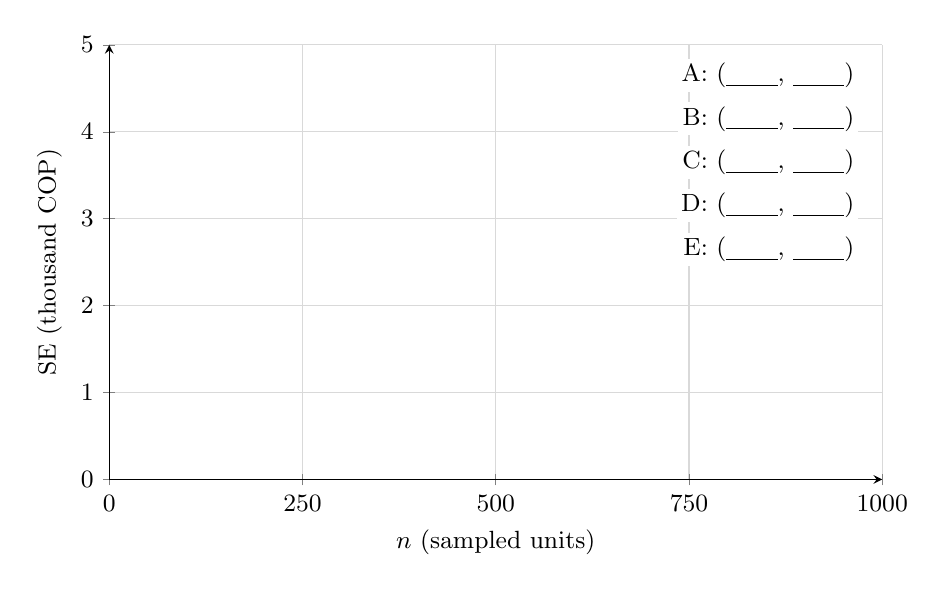
\begin{tikzpicture}\begin{axis}[relation,xlabel={$n$ (sampled units)},ylabel={SE (thousand COP)},xmin=0,xmax=1000,ymin=0,ymax=5,xtick={0,250,500,750,1000}]
\LabelTemplates
\end{axis}\end{tikzpicture}\end{minipage}
\hfill
\begin{minipage}[t]{.49\linewidth}\vspace{0pt}\centering\textbf{Margin of error vs sample size}\par
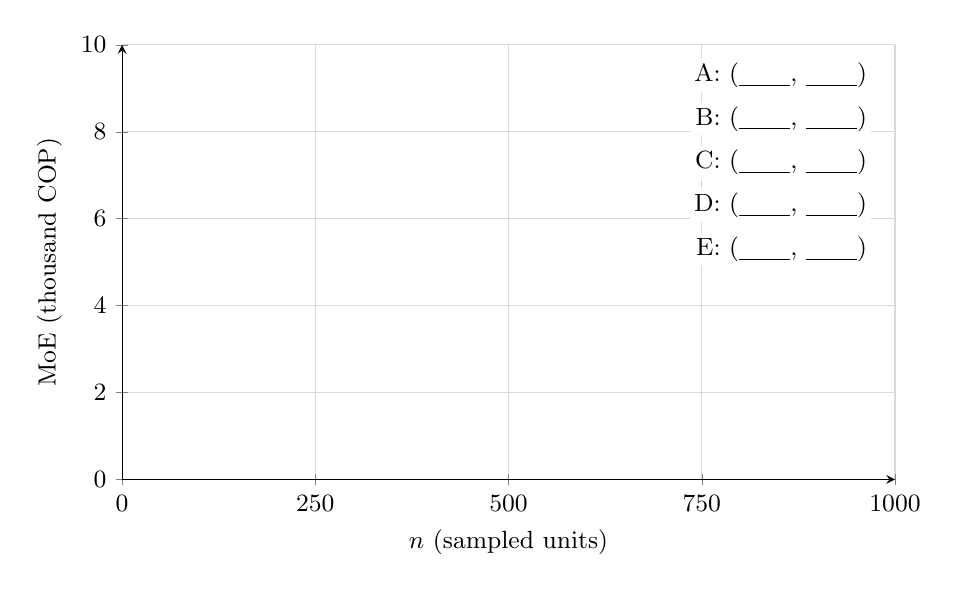
\begin{tikzpicture}\begin{axis}[relation,xlabel={$n$ (sampled units)},ylabel={MoE (thousand COP)},xmin=0,xmax=1000,ymin=0,ymax=10,xtick={0,250,500,750,1000}]
\LabelTemplates
\end{axis}\end{tikzpicture}\end{minipage}
\par\medskip
\begin{minipage}[t]{.49\linewidth}\vspace{0pt}\centering\textbf{Margin of error vs standard error}\par\smallskip
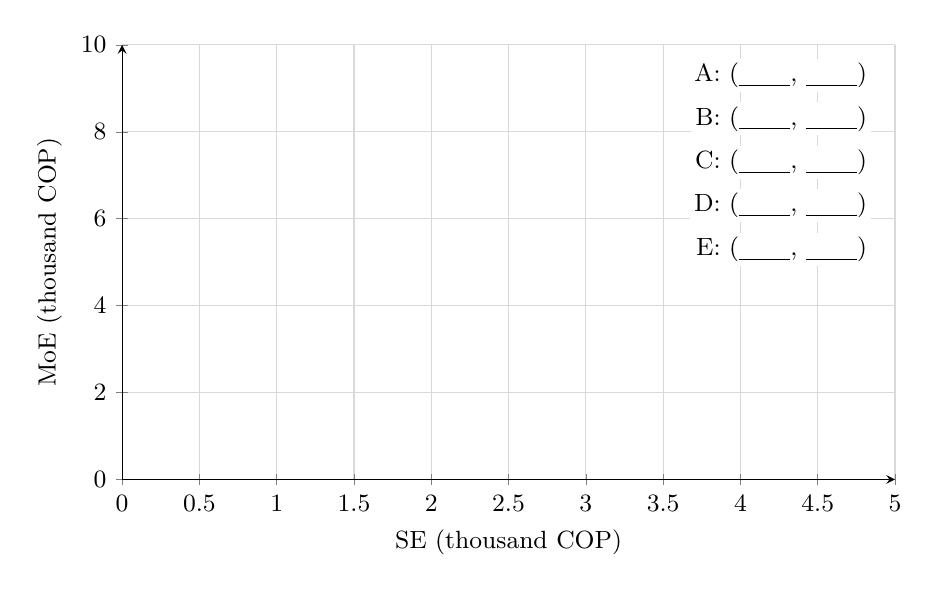
\begin{tikzpicture}\begin{axis}[relation,xlabel={SE (thousand COP)},ylabel={MoE (thousand COP)},xmin=0,xmax=5,ymin=0,ymax=10]
\LabelTemplates
\end{axis}\end{tikzpicture}\end{minipage}
\hfill\workarea\par

\clearpage 

\textbf{Problem 2 --- Delivery charges for local businesses continued}
\task{Task 2:}{Apply general Task 2 with $n=100$ and the five general confidence cases.}
\par \vspace{-2mm}
\begin{minipage}[t]{.49\linewidth}\vspace{0pt}\centering\textbf{Confidence level vs margin of error}\par\smallskip
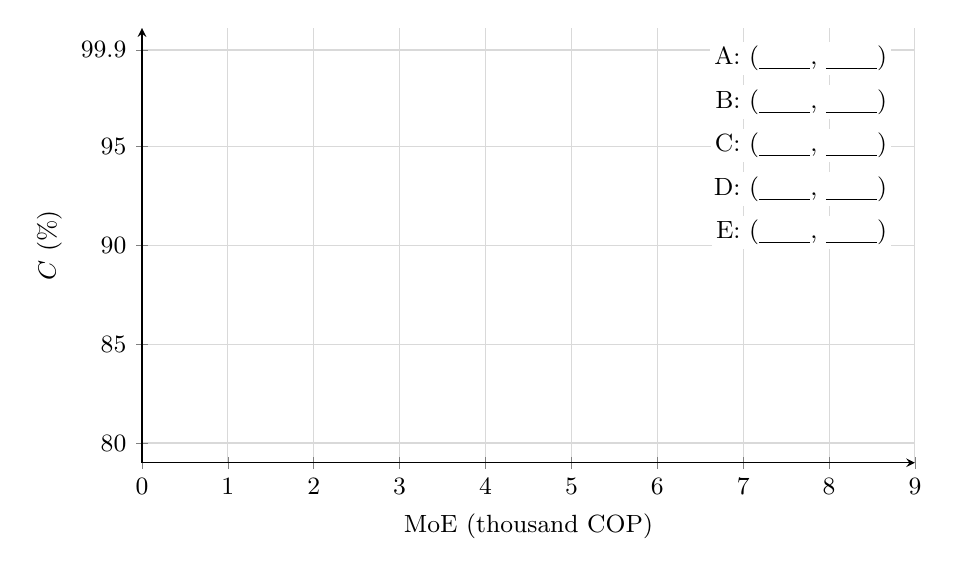
\begin{tikzpicture}\begin{axis}[relation,xlabel={MoE (thousand COP)},ylabel={$C$ (\%)},xmin=0,xmax=9,ymin=79,ymax=101,ytick={80,85,90,95,99.9}]
\LabelTemplates
\end{axis}\end{tikzpicture}\end{minipage}
\hfill
\begin{minipage}[t]{.49\linewidth}\vspace{0pt}\centering\textbf{Critical value vs margin of error}\par\smallskip
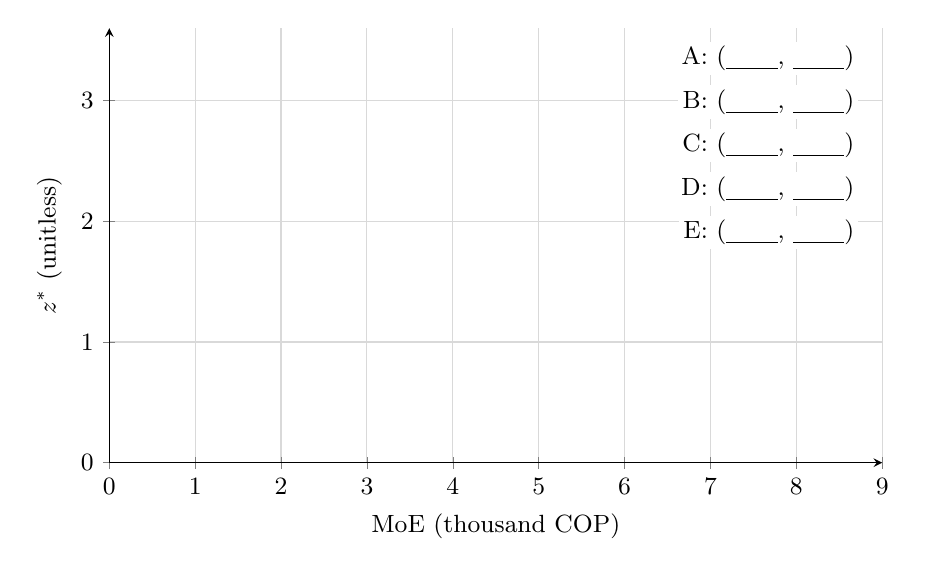
\begin{tikzpicture}\begin{axis}[relation,xlabel={MoE (thousand COP)},ylabel={$z^*$ (unitless)},xmin=0,xmax=9,ymin=0,ymax=3.6,ytick={0,1,2,3}]
\LabelTemplates
\end{axis}\end{tikzpicture}\end{minipage}
\par\medskip
\begin{minipage}[t]{.49\linewidth}\vspace{0pt}\centering\textbf{Confidence level vs critical value}\par\smallskip
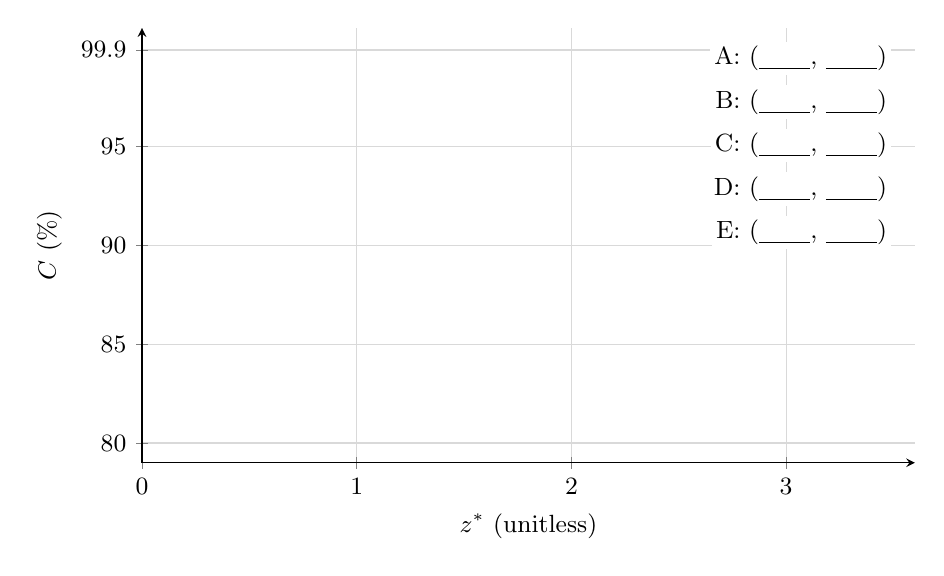
\begin{tikzpicture}\begin{axis}[relation,xlabel={$z^*$ (unitless)},ylabel={$C$ (\%)},xmin=0,xmax=3.6,ymin=79,ymax=101,xtick={0,1,2,3},ytick={80,85,90,95,99.9}]
\LabelTemplates
\end{axis}\end{tikzpicture}\end{minipage}
\hfill\workarea\par

\stageheading{Independent Practice}
\begingroup\small
\textit{Complete Independent Practice on a separate sheet.}\par

\problemtitle{3}{Weekly market-stall revenue}
A market office estimates mean weekly revenue per stall.
Population SD is known: $\sigma=45$ thousand COP; the common assumptions apply. For Task 1, fix $C=95\%$ ($z^*=1.960$) and use $n=25,100,225,625,1600$ for A--E, respectively. For Task 2, fix $n=225$ and the same $\sigma$, using the five general $(C,z^*)$ cases.
\task{Task 1:}{Calculate SE and MoE for cases A--E. Graph SE vs $n$, MoE vs $n$, and MoE vs SE, labelling all five cases with their coordinates and drawing the corresponding curves or lines.}

\task{Task 2:}{For the five general $(C,z^*)$ cases, calculate SE and MoE. Graph confidence vs MoE, critical value vs MoE, and confidence vs critical value, labelling all five cases with their coordinates and drawing the corresponding curves or lines.}

\problemtitle{4}{Freight handling fees}
A port analyst estimates the mean handling fee per container.
Population SD is known: $\sigma=72$ USD; the common assumptions apply. For Task 1, fix $C=95\%$ ($z^*=1.960$) and use $n=36,144,324,576,1296$ for A--E, respectively. For Task 2, fix $n=144$ and the same $\sigma$, using the five general $(C,z^*)$ cases.
\task{Task 1:}{Calculate SE and MoE for cases A--E. Graph SE vs $n$, MoE vs $n$, and MoE vs SE, labelling all five cases with their coordinates and drawing the corresponding curves or lines.}

\task{Task 2:}{For the five general $(C,z^*)$ cases, calculate SE and MoE. Graph confidence vs MoE, critical value vs MoE, and confidence vs critical value, labelling all five cases with their coordinates and drawing the corresponding curves or lines.}

\problemtitle{5}{Monthly internet costs}
A district estimates mean monthly internet expenditure per small business.
Population SD is known: $\sigma=35$ thousand COP; the common assumptions apply. For Task 1, fix $C=95\%$ ($z^*=1.960$) and use $n=49,100,196,400,1225$ for A--E, respectively. For Task 2, fix $n=196$ and the same $\sigma$, using the five general $(C,z^*)$ cases.
\task{Task 1:}{Calculate SE and MoE for cases A--E. Graph SE vs $n$, MoE vs $n$, and MoE vs SE, labelling all five cases with their coordinates and drawing the corresponding curves or lines.}

\task{Task 2:}{For the five general $(C,z^*)$ cases, calculate SE and MoE. Graph confidence vs MoE, critical value vs MoE, and confidence vs critical value, labelling all five cases with their coordinates and drawing the corresponding curves or lines.}
\par\endgroup
\clearpage
% All palette, graph and spacing choices below are local to the solutions.
\begingroup
\CoordinatedTermTwoPalette
\setlength{\parskip}{5pt}
\ifGTenHighlights
  \colorlet{CthreeSELine}{CtwoSEColor!55!black}
  \colorlet{CthreeMoELine}{CtwoMoEColor!75!black}
  \colorlet{CthreeCriticalLine}{CtwoCriticalColor}
  \colorlet{CthreeConfidenceLine}{CtwoConfidenceColor!50!black}
  \colorlet{CthreeConfidenceFill}{CtwoConfidenceColor!32!white}
\else
  \colorlet{CthreeSELine}{black}
  \colorlet{CthreeMoELine}{black}
  \colorlet{CthreeCriticalLine}{black}
  \colorlet{CthreeConfidenceLine}{black}
  \colorlet{CthreeConfidenceFill}{black!12}
\fi
\pgfplotsset{c3axis/.style={width=.89\linewidth,height=6.3cm,
  axis x line=bottom,axis y line=middle,grid=major,major grid style={black!12},
  tick label style={font=\small},label style={font=\small},
  scaled ticks=false,unbounded coords=jump,
  every axis plot/.append style={thick},enlarge x limits=false,
  title style={font=\normalsize},clip=true}}

% Coordinates retain their original precision; only printed values are rounded.
% Each call places a label separately and joins its nearest edge to the marker.
\newcommand{\CthreePointLabel}[7]{%
  \node[font=\scriptsize,inner sep=2pt,anchor=#7] (c3point#1)
    at (axis description cs:#5,#6) {% Keep coordinate highlights within the original label footprint.
      \tikzset{gten marker/.append style={inner xsep=.4mm}}%
      #1: $(#3,\,#4)$};
  \draw[black!70,line width=.35pt,shorten <=2.5pt]
    (axis cs:#2) -- (c3point#1);
}

\section*{Solutions}
\textbf{Problems 2--5: guided example and independent practice.}
All calculations use the activity's supplied data and critical values. Monetary
results are in thousand COP except Problem 4, which uses USD. Sample sizes count
sampled units; critical values are unitless.

\textbf{Highlight guide.} The following roles reuse the reference's shared definitions.
\begin{center}
\begin{tabular}{lll}\toprule
Symbol & Concept & Meaning in these solutions\\\midrule
$\CtwoSize{n}$ & \CtwoSize{Sample size} & Number of observations\\
$\CtwoSD{\sigma}$ & \CtwoSD{Population SD} & Known spread of individual values\\
$\CtwoSE{\mathrm{SE}}$ & \CtwoSE{Standard error} & Uncertainty in the sample mean\\
$\CtwoConfidence{C}$ & \CtwoConfidence{Nominal confidence} & Supplied percentage on the graphs\\
$\CtwoCritical{z^*}$ & \CtwoCritical{Critical value} & Supplied rounded normal cutoff\\
$\CtwoMoE{\mathrm{MoE}}$ & \CtwoMoE{Margin of error} & Distance from centre to an endpoint\\
$\HLCumulativeProbability{C_{\rm normal}}$ & \HLCumulativeProbability{Theoretical coverage} & Central normal area from rounded cutoff\\\bottomrule
\end{tabular}
\end{center}
\textbf{Formulas and rounding.}
\[
\CtwoSE{\mathrm{SE}}=\frac{\CtwoSD{\sigma}}{\sqrt{\CtwoSize{n}}},\qquad
\CtwoMoE{\mathrm{MoE}}=\CtwoCritical{z^*}\CtwoSE{\mathrm{SE}},\qquad
\CtwoWidth{W}=2\CtwoMoE{\mathrm{MoE}}.
\]
Keep full precision in all intermediate calculations; displayed monetary values
and calculated coordinates use three decimals. Here the supplied sample sizes are
perfect squares and all intermediate SE values are exact terminating decimals.
No point estimate is supplied for Problems 2--5, so numerical interval endpoints
cannot be computed. An interval has the symbolic form
$\CtwoPoint{\bar{x}}\pm\CtwoMoE{\mathrm{MoE}}$.

\textbf{Nominal confidence and theoretical coverage.} Let $\Phi$ be the standard
normal cumulative distribution function. The smooth confidence curves use
\[
\HLCumulativeProbability{C_{\rm normal}}(\%)=
100[2\Phi(\CtwoCritical{z^*})-1]
=100[2\Phi(\CtwoMoE{\mathrm{MoE}}/\CtwoSE{\mathrm{SE}})-1].
\]
The plotted markers retain the \CtwoConfidence{nominal supplied percentages}.
Their rounded cutoffs give the slightly different theoretical coverages below;
five decimal places make the rounding differences visible.
\begin{center}\begin{tabular}{lrrl}\toprule
Case & $\CtwoConfidence{C}$ (\%) & $\CtwoCritical{z^*}$ & $\HLCumulativeProbability{C_{\rm normal}}$ (\%)\\\midrule
A & \CtwoConfidence{80} & \CtwoCritical{1.282} & $100[2\Phi(\CtwoCritical{1.282})-1]\approx\HLCumulativeProbability{80.01574}$\\
B & \CtwoConfidence{90} & \CtwoCritical{1.645} & $100[2\Phi(\CtwoCritical{1.645})-1]\approx\HLCumulativeProbability{90.00302}$\\
C & \CtwoConfidence{95} & \CtwoCritical{1.960} & $100[2\Phi(\CtwoCritical{1.960})-1]\approx\HLCumulativeProbability{95.00042}$\\
D & \CtwoConfidence{99} & \CtwoCritical{2.576} & $100[2\Phi(\CtwoCritical{2.576})-1]\approx\HLCumulativeProbability{99.00049}$\\
E & \CtwoConfidence{99.9} & \CtwoCritical{3.291} & $100[2\Phi(\CtwoCritical{3.291})-1]\approx\HLCumulativeProbability{99.90017}$\\
\bottomrule\end{tabular}\end{center}
Confidence describes long-run coverage of the fixed population mean under the
sampling model; it is not a probability assigned to that mean after observing an
interval. Higher confidence requires a larger margin at fixed SE.

\textbf{Graph convention.} ``A vs B'' places A vertically and B horizontally.
Filled markers are the five supplied cases. Smooth lines use the formulas;
the continuous sample-size curve is a guide between feasible integer sizes.
Coordinate labels are rounded only for display.
\clearpage
\begin{landscape}
\textbf{Problem 2 --- Delivery charges for local businesses}\par
\textbf{Task 1 -- Vary sample size}\par
Hold $\CtwoSD{\sigma}=\CtwoSD{24}$ thousand COP and $\CtwoConfidence{C}=\CtwoConfidence{95\%}$ ($\CtwoCritical{z^*}=\CtwoCritical{1.960}$) fixed.
Use $\CtwoSE{\mathrm{SE}}=\CtwoSD{24}/\sqrt{\CtwoSize{n}}$ and $\CtwoMoE{\mathrm{MoE}}=\CtwoCritical{1.960}(\CtwoSD{24}/\sqrt{\CtwoSize{n}})$, in thousand COP.\par
\par\medskip
\noindent\begin{minipage}[t]{.55\linewidth}\vspace{0pt}
\begin{tikzpicture}
\begin{axis}[c3axis,width=.82\linewidth,height=10cm,scale only axis,title={Standard error vs sample size},xlabel={$\CtwoSize{n}$ (sampled units)},ylabel={$\CtwoSE{\mathrm{SE}}$ (thousand COP)},xmin=0,xmax=972.0000000000001,ymin=0,ymax=4.8]
\addplot[CthreeSELine,domain=36:900,samples=180] {24/sqrt(x)};
\addplot[only marks,mark=*,mark size=2.2pt,CthreeSELine] coordinates {(36.000000000000,4.000000000000) (100.000000000000,2.400000000000) (225.000000000000,1.600000000000) (400.000000000000,1.200000000000) (900.000000000000,0.800000000000)};
\CthreePointLabel{A}{36.000000000000,4.000000000000}{\CtwoSize{36}}{\CtwoSE{4.000}}{0.19}{0.91}{west}
\CthreePointLabel{B}{100.000000000000,2.400000000000}{\CtwoSize{100}}{\CtwoSE{2.400}}{0.28}{0.74}{west}
\CthreePointLabel{C}{225.000000000000,1.600000000000}{\CtwoSize{225}}{\CtwoSE{1.600}}{0.4}{0.57}{west}
\CthreePointLabel{D}{400.000000000000,1.200000000000}{\CtwoSize{400}}{\CtwoSE{1.200}}{0.64}{0.4}{west}
\CthreePointLabel{E}{900.000000000000,0.800000000000}{\CtwoSize{900}}{\CtwoSE{0.800}}{0.98}{0.24}{east}
\end{axis}\end{tikzpicture}
\end{minipage}\hfill
\begin{minipage}[t]{.43\linewidth}\vspace{0pt}
\centering\small
\textbf{Plotted points and calculations}\par\medskip
\setlength{\tabcolsep}{3pt}\renewcommand{\arraystretch}{1.18}
\setlength{\jot}{1pt}
\begin{tabular}{@{}lrrl@{}}\toprule
ID & $\CtwoSize{n}$ & $\CtwoSE{\mathrm{SE}}$ & Calculation\\\midrule
A & \CtwoSize{36} & \CtwoSE{4.000} & $\begin{aligned}[t]&\CtwoSD{24}/\sqrt{\CtwoSize{36}}\\ &=\CtwoSD{24}/\CtwoSize{6}\\ &=\CtwoSE{4.000}\end{aligned}$\\[5pt]
B & \CtwoSize{100} & \CtwoSE{2.400} & $\begin{aligned}[t]&\CtwoSD{24}/\sqrt{\CtwoSize{100}}\\ &=\CtwoSD{24}/\CtwoSize{10}\\ &=\CtwoSE{2.400}\end{aligned}$\\[5pt]
C & \CtwoSize{225} & \CtwoSE{1.600} & $\begin{aligned}[t]&\CtwoSD{24}/\sqrt{\CtwoSize{225}}\\ &=\CtwoSD{24}/\CtwoSize{15}\\ &=\CtwoSE{1.600}\end{aligned}$\\[5pt]
D & \CtwoSize{400} & \CtwoSE{1.200} & $\begin{aligned}[t]&\CtwoSD{24}/\sqrt{\CtwoSize{400}}\\ &=\CtwoSD{24}/\CtwoSize{20}\\ &=\CtwoSE{1.200}\end{aligned}$\\[5pt]
E & \CtwoSize{900} & \CtwoSE{0.800} & $\begin{aligned}[t]&\CtwoSD{24}/\sqrt{\CtwoSize{900}}\\ &=\CtwoSD{24}/\CtwoSize{30}\\ &=\CtwoSE{0.800}\end{aligned}$\\[5pt]
\bottomrule\end{tabular}\par\medskip\raggedright
Columns follow the axes. SE and MoE: thousand COP; $n$: sampled units; $C$: nominal percent; $z^*$: unitless. Calculations and drawing coordinates retain full precision; printed monetary coordinates use three decimals.
\end{minipage}\par\bigskip
\textbf{Interpretation.} As \CtwoSize{sample size} increases, \CtwoSE{standard error} decreases as $1/\sqrt{\CtwoSize{n}}$. Quadrupling the size halves SE: more observations improve precision, with unchanged population variability and confidence.
\end{landscape}
\clearpage
\begin{landscape}
\textbf{Problem 2 --- Delivery charges for local businesses}\par
\textbf{Task 1 -- Vary sample size}\par
Hold $\CtwoSD{\sigma}=\CtwoSD{24}$ thousand COP and $\CtwoConfidence{C}=\CtwoConfidence{95\%}$ ($\CtwoCritical{z^*}=\CtwoCritical{1.960}$) fixed.
Use $\CtwoSE{\mathrm{SE}}=\CtwoSD{24}/\sqrt{\CtwoSize{n}}$ and $\CtwoMoE{\mathrm{MoE}}=\CtwoCritical{1.960}(\CtwoSD{24}/\sqrt{\CtwoSize{n}})$, in thousand COP.\par
\par\medskip
\noindent\begin{minipage}[t]{.55\linewidth}\vspace{0pt}
\begin{tikzpicture}
\begin{axis}[c3axis,width=.82\linewidth,height=10cm,scale only axis,title={Margin of error vs sample size},xlabel={$\CtwoSize{n}$ (sampled units)},ylabel={$\CtwoMoE{\mathrm{MoE}}$ (thousand COP)},xmin=0,xmax=972.0000000000001,ymin=0,ymax=9.408]
\addplot[CthreeMoELine,domain=36:900,samples=180] {1.960*24/sqrt(x)};
\addplot[only marks,mark=*,mark size=2.2pt,CthreeMoELine] coordinates {(36.000000000000,7.840000000000) (100.000000000000,4.704000000000) (225.000000000000,3.136000000000) (400.000000000000,2.352000000000) (900.000000000000,1.568000000000)};
\CthreePointLabel{A}{36.000000000000,7.840000000000}{\CtwoSize{36}}{\CtwoMoE{7.840}}{0.19}{0.91}{west}
\CthreePointLabel{B}{100.000000000000,4.704000000000}{\CtwoSize{100}}{\CtwoMoE{4.704}}{0.28}{0.74}{west}
\CthreePointLabel{C}{225.000000000000,3.136000000000}{\CtwoSize{225}}{\CtwoMoE{3.136}}{0.4}{0.57}{west}
\CthreePointLabel{D}{400.000000000000,2.352000000000}{\CtwoSize{400}}{\CtwoMoE{2.352}}{0.64}{0.4}{west}
\CthreePointLabel{E}{900.000000000000,1.568000000000}{\CtwoSize{900}}{\CtwoMoE{1.568}}{0.98}{0.24}{east}
\end{axis}\end{tikzpicture}
\end{minipage}\hfill
\begin{minipage}[t]{.43\linewidth}\vspace{0pt}
\centering\small
\textbf{Plotted points and calculations}\par\medskip
\setlength{\tabcolsep}{3pt}\renewcommand{\arraystretch}{1.18}
\setlength{\jot}{1pt}
\begin{tabular}{@{}lrrl@{}}\toprule
ID & $\CtwoSize{n}$ & $\CtwoMoE{\mathrm{MoE}}$ & Calculation\\\midrule
A & \CtwoSize{36} & \CtwoMoE{7.840} & $\begin{aligned}[t]&\CtwoCritical{1.960}(\CtwoSD{24}/\sqrt{\CtwoSize{36}})\\ &=\CtwoCritical{1.960}(\CtwoSE{4.000})\\ &=\CtwoMoE{7.840}\end{aligned}$\\[5pt]
B & \CtwoSize{100} & \CtwoMoE{4.704} & $\begin{aligned}[t]&\CtwoCritical{1.960}(\CtwoSD{24}/\sqrt{\CtwoSize{100}})\\ &=\CtwoCritical{1.960}(\CtwoSE{2.400})\\ &=\CtwoMoE{4.704}\end{aligned}$\\[5pt]
C & \CtwoSize{225} & \CtwoMoE{3.136} & $\begin{aligned}[t]&\CtwoCritical{1.960}(\CtwoSD{24}/\sqrt{\CtwoSize{225}})\\ &=\CtwoCritical{1.960}(\CtwoSE{1.600})\\ &=\CtwoMoE{3.136}\end{aligned}$\\[5pt]
D & \CtwoSize{400} & \CtwoMoE{2.352} & $\begin{aligned}[t]&\CtwoCritical{1.960}(\CtwoSD{24}/\sqrt{\CtwoSize{400}})\\ &=\CtwoCritical{1.960}(\CtwoSE{1.200})\\ &=\CtwoMoE{2.352}\end{aligned}$\\[5pt]
E & \CtwoSize{900} & \CtwoMoE{1.568} & $\begin{aligned}[t]&\CtwoCritical{1.960}(\CtwoSD{24}/\sqrt{\CtwoSize{900}})\\ &=\CtwoCritical{1.960}(\CtwoSE{0.800})\\ &=\CtwoMoE{1.568}\end{aligned}$\\[5pt]
\bottomrule\end{tabular}\par\medskip\raggedright
Columns follow the axes. SE and MoE: thousand COP; $n$: sampled units; $C$: nominal percent; $z^*$: unitless. Calculations and drawing coordinates retain full precision; printed monetary coordinates use three decimals.
\end{minipage}\par\bigskip
\textbf{Interpretation.} At fixed \CtwoConfidence{confidence}, \CtwoMoE{margin of error} decreases as $1/\sqrt{\CtwoSize{n}}$. Quadrupling sample size halves the margin and interval width, giving greater precision at the same nominal coverage.
\end{landscape}
\clearpage
\begin{landscape}
\textbf{Problem 2 --- Delivery charges for local businesses}\par
\textbf{Task 1 -- Vary sample size}\par
Hold $\CtwoSD{\sigma}=\CtwoSD{24}$ thousand COP and $\CtwoConfidence{C}=\CtwoConfidence{95\%}$ ($\CtwoCritical{z^*}=\CtwoCritical{1.960}$) fixed.
Use $\CtwoSE{\mathrm{SE}}=\CtwoSD{24}/\sqrt{\CtwoSize{n}}$ and $\CtwoMoE{\mathrm{MoE}}=\CtwoCritical{1.960}(\CtwoSD{24}/\sqrt{\CtwoSize{n}})$, in thousand COP.\par
\par\medskip
\noindent\begin{minipage}[t]{.55\linewidth}\vspace{0pt}
\begin{tikzpicture}
\begin{axis}[c3axis,width=.82\linewidth,height=10cm,scale only axis,title={Margin of error vs standard error},xlabel={$\CtwoSE{\mathrm{SE}}$ (thousand COP)},ylabel={$\CtwoMoE{\mathrm{MoE}}$ (thousand COP)},xmin=0,xmax=4.6,ymin=0,ymax=9.408]
\addplot[CthreeMoELine,domain=0:4.24] {1.960*x};
\addplot[only marks,mark=*,mark size=2.2pt,CthreeMoELine] coordinates {(4.000000000000,7.840000000000) (2.400000000000,4.704000000000) (1.600000000000,3.136000000000) (1.200000000000,2.352000000000) (0.800000000000,1.568000000000)};
\CthreePointLabel{A}{4.000000000000,7.840000000000}{\CtwoSE{4.000}}{\CtwoMoE{7.840}}{0.53}{0.92}{west}
\CthreePointLabel{B}{2.400000000000,4.704000000000}{\CtwoSE{2.400}}{\CtwoMoE{4.704}}{0.41}{0.81}{west}
\CthreePointLabel{C}{1.600000000000,3.136000000000}{\CtwoSE{1.600}}{\CtwoMoE{3.136}}{0.29}{0.7}{west}
\CthreePointLabel{D}{1.200000000000,2.352000000000}{\CtwoSE{1.200}}{\CtwoMoE{2.352}}{0.17}{0.59}{west}
\CthreePointLabel{E}{0.800000000000,1.568000000000}{\CtwoSE{0.800}}{\CtwoMoE{1.568}}{0.05}{0.48}{west}
\end{axis}\end{tikzpicture}
\end{minipage}\hfill
\begin{minipage}[t]{.43\linewidth}\vspace{0pt}
\centering\small
\textbf{Plotted points and calculations}\par\medskip
\setlength{\tabcolsep}{3pt}\renewcommand{\arraystretch}{1.18}
\setlength{\jot}{1pt}
\begin{tabular}{@{}lrrl@{}}\toprule
ID & $\CtwoSE{\mathrm{SE}}$ & $\CtwoMoE{\mathrm{MoE}}$ & Calculation\\\midrule
A & \CtwoSE{4.000} & \CtwoMoE{7.840} & $\begin{aligned}[t]&\CtwoCritical{1.960}(\CtwoSE{4.000})\\ &=\CtwoMoE{7.840}\end{aligned}$\\[5pt]
B & \CtwoSE{2.400} & \CtwoMoE{4.704} & $\begin{aligned}[t]&\CtwoCritical{1.960}(\CtwoSE{2.400})\\ &=\CtwoMoE{4.704}\end{aligned}$\\[5pt]
C & \CtwoSE{1.600} & \CtwoMoE{3.136} & $\begin{aligned}[t]&\CtwoCritical{1.960}(\CtwoSE{1.600})\\ &=\CtwoMoE{3.136}\end{aligned}$\\[5pt]
D & \CtwoSE{1.200} & \CtwoMoE{2.352} & $\begin{aligned}[t]&\CtwoCritical{1.960}(\CtwoSE{1.200})\\ &=\CtwoMoE{2.352}\end{aligned}$\\[5pt]
E & \CtwoSE{0.800} & \CtwoMoE{1.568} & $\begin{aligned}[t]&\CtwoCritical{1.960}(\CtwoSE{0.800})\\ &=\CtwoMoE{1.568}\end{aligned}$\\[5pt]
\bottomrule\end{tabular}\par\medskip\raggedright
Columns follow the axes. SE and MoE: thousand COP; $n$: sampled units; $C$: nominal percent; $z^*$: unitless. Calculations and drawing coordinates retain full precision; printed monetary coordinates use three decimals.
\end{minipage}\par\bigskip
\textbf{Interpretation.} The relationship is a line through the origin: $\CtwoMoE{\mathrm{MoE}}=\CtwoCritical{1.960}\CtwoSE{\mathrm{SE}}$. Its slope is the fixed, unitless critical value. Halving SE halves the margin; the two axes have the same monetary unit.
\end{landscape}
\clearpage
\begin{landscape}
\textbf{Problem 2 --- Delivery charges for local businesses}\par
\textbf{Task 2 -- Vary confidence}\par
Hold $\CtwoSD{\sigma}=\CtwoSD{24}$ thousand COP and $\CtwoSize{n}=\CtwoSize{100}$ fixed.
Then $\CtwoSE{\mathrm{SE}}=\CtwoSD{24}/\sqrt{\CtwoSize{100}}=\CtwoSD{24}/\CtwoSize{10}=\CtwoSE{2.400}$ thousand COP; $\CtwoMoE{\mathrm{MoE}}=\CtwoCritical{z^*}(\CtwoSE{2.400})$.\par
\par\medskip
\noindent\begin{minipage}[t]{.55\linewidth}\vspace{0pt}
\begin{tikzpicture}
\begin{axis}[c3axis,width=.82\linewidth,height=10cm,scale only axis,title={Confidence level vs margin of error},xlabel={$\CtwoMoE{\mathrm{MoE}}$ (thousand COP)},ylabel={$\CtwoConfidence{C}$ (\%)},xmin=0,xmax=8.68824,ymin=79,ymax=101,ytick={80,85,90,95,99.9}]
\addplot[CthreeConfidenceLine] coordinates {(2.880000000000,76.986065955658) (2.909333333333,77.457267281357) (2.938666666667,77.921538814053) (2.968000000000,78.378914139566) (2.997333333333,78.829428389706) (3.026666666667,79.273118203571) (3.056000000000,79.710021688533) (3.085333333333,80.140178380943) (3.114666666667,80.563629206591) (3.144000000000,80.980416440952) (3.173333333333,81.390583669251) (3.202666666667,81.794175746381) (3.232000000000,82.191238756705) (3.261333333333,82.581819973775) (3.290666666667,82.965967819994) (3.320000000000,83.343731826261) (3.349333333333,83.715162591619) (3.378666666667,84.080311742941) (3.408000000000,84.439231894691) (3.437333333333,84.791976608767) (3.466666666667,85.138600354479) (3.496000000000,85.479158468673) (3.525333333333,85.813707116034) (3.554666666667,86.142303249594) (3.584000000000,86.465004571467) (3.613333333333,86.781869493846) (3.642666666667,87.092957100271) (3.672000000000,87.398327107204) (3.701333333333,87.698039825933) (3.730666666667,87.992156124816) (3.760000000000,88.280737391903) (3.789333333333,88.563845497943) (3.818666666667,88.841542759803) (3.848000000000,89.113891904318) (3.877333333333,89.380956032589) (3.906666666667,89.642798584742) (3.936000000000,89.899483305179) (3.965333333333,90.151074208324) (3.994666666667,90.397635544880) (4.024000000000,90.639231768623) (4.053333333333,90.875927503735) (4.082666666667,91.107787512697) (4.112000000000,91.334876664747) (4.141333333333,91.557259904925) (4.170666666667,91.775002223706) (4.200000000000,91.988168627237) (4.229333333333,92.196824108182) (4.258666666667,92.401033617198) (4.288000000000,92.600862035025) (4.317333333333,92.796374145226) (4.346666666667,92.987634607557) (4.376000000000,93.174707931996) (4.405333333333,93.357658453416) (4.434666666667,93.536550306922) (4.464000000000,93.711447403849) (4.493333333333,93.882413408423) (4.522666666667,94.049511715087) (4.552000000000,94.212805426501) (4.581333333333,94.372357332208) (4.610666666667,94.528229887975) (4.640000000000,94.680485195798) (4.669333333333,94.829184984582) (4.698666666667,94.974390591491) (4.728000000000,95.116162943956) (4.757333333333,95.254562542360) (4.786666666667,95.389649443375) (4.816000000000,95.521483243962) (4.845333333333,95.650123066022) (4.874666666667,95.775627541701) (4.904000000000,95.898054799336) (4.933333333333,96.017462450045) (4.962666666667,96.133907574947) (4.992000000000,96.247446713012) (5.021333333333,96.358135849534) (5.050666666667,96.466030405212) (5.080000000000,96.571185225846) (5.109333333333,96.673654572630) (5.138666666667,96.773492113030) (5.168000000000,96.870750912254) (5.197333333333,96.965483425293) (5.226666666667,97.057741489521) (5.256000000000,97.147576317866) (5.285333333333,97.235038492512) (5.314666666667,97.320177959147) (5.344000000000,97.403044021737) (5.373333333333,97.483685337814) (5.402666666667,97.562149914279) (5.432000000000,97.638485103685) (5.461333333333,97.712737601027) (5.490666666667,97.784953440989) (5.520000000000,97.855177995665) (5.549333333333,97.923455972727) (5.578666666667,97.989831414043) (5.608000000000,98.054347694716) (5.637333333333,98.117047522548) (5.666666666667,98.177972937914) (5.696000000000,98.237165314024) (5.725333333333,98.294665357584) (5.754666666667,98.350513109816) (5.784000000000,98.404747947853) (5.813333333333,98.457408586476) (5.842666666667,98.508533080197) (5.872000000000,98.558158825667) (5.901333333333,98.606322564400) (5.930666666667,98.653060385809) (5.960000000000,98.698407730529) (5.989333333333,98.742399394027) (6.018666666667,98.785069530482) (6.048000000000,98.826451656933) (6.077333333333,98.866578657670) (6.106666666667,98.905482788863) (6.136000000000,98.943195683434) (6.165333333333,98.979748356129) (6.194666666667,99.015171208812) (6.224000000000,99.049494035948) (6.253333333333,99.082746030281) (6.282666666667,99.114955788685) (6.312000000000,99.146151318182) (6.341333333333,99.176360042124) (6.370666666667,99.205608806515) (6.400000000000,99.233923886482) (6.429333333333,99.261330992867) (6.458666666667,99.287855278946) (6.488000000000,99.313521347263) (6.517333333333,99.338353256554) (6.546666666667,99.362374528787) (6.576000000000,99.385608156270) (6.605333333333,99.408076608847) (6.634666666667,99.429801841168) (6.664000000000,99.450805300013) (6.693333333333,99.471107931681) (6.722666666667,99.490730189424) (6.752000000000,99.509692040919) (6.781333333333,99.528012975782) (6.810666666667,99.545712013106) (6.840000000000,99.562807709017) (6.869333333333,99.579318164255) (6.898666666667,99.595261031754) (6.928000000000,99.610653524230) (6.957333333333,99.625512421769) (6.986666666667,99.639854079403) (7.016000000000,99.653694434672) (7.045333333333,99.667049015173) (7.074666666667,99.679932946083) (7.104000000000,99.692360957652) (7.133333333333,99.704347392668) (7.162666666667,99.715906213879) (7.192000000000,99.727051011384) (7.221333333333,99.737795009970) (7.250666666667,99.748151076402) (7.280000000000,99.758131726667) (7.309333333333,99.767749133155) (7.338666666667,99.777015131783) (7.368000000000,99.785941229064) (7.397333333333,99.794538609098) (7.426666666667,99.802818140506) (7.456000000000,99.810790383292) (7.485333333333,99.818465595629) (7.514666666667,99.825853740569) (7.544000000000,99.832964492685) (7.573333333333,99.839807244622) (7.602666666667,99.846391113577) (7.632000000000,99.852724947689) (7.661333333333,99.858817332349) (7.690666666667,99.864676596423) (7.720000000000,99.870310818391) (7.749333333333,99.875727832391) (7.778666666667,99.880935234182) (7.808000000000,99.885940387012) (7.837333333333,99.890750427395) (7.866666666667,99.895372270799) (7.896000000000,99.899812617243) (7.925333333333,99.904077956792) (7.954666666667,99.908174574972) (7.984000000000,99.912108558083) (8.013333333333,99.915885798422) (8.042666666667,99.919511999407) (8.072000000000,99.922992680619) (8.101333333333,99.926333182733) (8.130666666667,99.929538672374) (8.160000000000,99.932614146865)};
\addplot[only marks,mark=*,mark size=2.2pt,CthreeConfidenceLine] coordinates {(3.076800000000,80.000000000000) (3.948000000000,90.000000000000) (4.704000000000,95.000000000000) (6.182400000000,99.000000000000) (7.898400000000,99.900000000000)};
\CthreePointLabel{A}{3.076800000000,80.000000000000}{\CtwoMoE{3.077}}{\CtwoConfidence{80}}{0.36}{0.13}{east}
\CthreePointLabel{B}{3.948000000000,90.000000000000}{\CtwoMoE{3.948}}{\CtwoConfidence{90}}{0.44}{0.39}{east}
\CthreePointLabel{C}{4.704000000000,95.000000000000}{\CtwoMoE{4.704}}{\CtwoConfidence{95}}{0.52}{0.62}{east}
\CthreePointLabel{D}{6.182400000000,99.000000000000}{\CtwoMoE{6.182}}{\CtwoConfidence{99}}{0.7}{0.82}{east}
\CthreePointLabel{E}{7.898400000000,99.900000000000}{\CtwoMoE{7.898}}{\CtwoConfidence{99.9}}{0.98}{0.55}{east}
\end{axis}\end{tikzpicture}
\end{minipage}\hfill
\begin{minipage}[t]{.43\linewidth}\vspace{0pt}
\centering\small
\textbf{Plotted points and calculations}\par\medskip
\setlength{\tabcolsep}{3pt}\renewcommand{\arraystretch}{1.18}
\setlength{\jot}{1pt}
\begin{tabular}{@{}lrrl@{}}\toprule
ID & $\CtwoMoE{\mathrm{MoE}}$ & $\CtwoConfidence{C}$ & Calculation\\\midrule
A & \CtwoMoE{3.077} & \CtwoConfidence{80} & $\begin{aligned}[t]&\CtwoMoE{\mathrm{MoE}}=\CtwoCritical{1.282}(\CtwoSE{2.400})=\CtwoMoE{3.0768}\\ &100[2\Phi(\CtwoMoE{3.0768}/\CtwoSE{2.400})-1]\\ &\approx\HLCumulativeProbability{80.01574\%}\end{aligned}$\\[5pt]
B & \CtwoMoE{3.948} & \CtwoConfidence{90} & $\begin{aligned}[t]&\CtwoMoE{\mathrm{MoE}}=\CtwoCritical{1.645}(\CtwoSE{2.400})=\CtwoMoE{3.948}\\ &100[2\Phi(\CtwoMoE{3.948}/\CtwoSE{2.400})-1]\\ &\approx\HLCumulativeProbability{90.00302\%}\end{aligned}$\\[5pt]
C & \CtwoMoE{4.704} & \CtwoConfidence{95} & $\begin{aligned}[t]&\CtwoMoE{\mathrm{MoE}}=\CtwoCritical{1.960}(\CtwoSE{2.400})=\CtwoMoE{4.704}\\ &100[2\Phi(\CtwoMoE{4.704}/\CtwoSE{2.400})-1]\\ &\approx\HLCumulativeProbability{95.00042\%}\end{aligned}$\\[5pt]
D & \CtwoMoE{6.182} & \CtwoConfidence{99} & $\begin{aligned}[t]&\CtwoMoE{\mathrm{MoE}}=\CtwoCritical{2.576}(\CtwoSE{2.400})=\CtwoMoE{6.1824}\\ &100[2\Phi(\CtwoMoE{6.1824}/\CtwoSE{2.400})-1]\\ &\approx\HLCumulativeProbability{99.00049\%}\end{aligned}$\\[5pt]
E & \CtwoMoE{7.898} & \CtwoConfidence{99.9} & $\begin{aligned}[t]&\CtwoMoE{\mathrm{MoE}}=\CtwoCritical{3.291}(\CtwoSE{2.400})=\CtwoMoE{7.8984}\\ &100[2\Phi(\CtwoMoE{7.8984}/\CtwoSE{2.400})-1]\\ &\approx\HLCumulativeProbability{99.90017\%}\end{aligned}$\\[5pt]
\bottomrule\end{tabular}\par\medskip\raggedright
Columns follow the axes. SE and MoE: thousand COP; $n$: sampled units; $C$: nominal percent; $z^*$: unitless. Calculations and drawing coordinates retain full precision; printed monetary coordinates use three decimals.
The calculation gives theoretical normal coverage, not the nominal percentage in the $\CtwoConfidence{C}$ column. Five coverage decimals expose cutoff rounding.
\end{minipage}\par\bigskip
\textbf{Interpretation.} With \CtwoSE{SE} fixed, higher \CtwoConfidence{confidence} requires a larger \CtwoMoE{margin}, so intervals widen and precision decreases. The nonlinear curve flattens toward 100\%; its theoretical coverage differs slightly from the nominal markers because the supplied cutoffs are rounded.
\end{landscape}
\clearpage
\begin{landscape}
\textbf{Problem 2 --- Delivery charges for local businesses}\par
\textbf{Task 2 -- Vary confidence}\par
Hold $\CtwoSD{\sigma}=\CtwoSD{24}$ thousand COP and $\CtwoSize{n}=\CtwoSize{100}$ fixed.
Then $\CtwoSE{\mathrm{SE}}=\CtwoSD{24}/\sqrt{\CtwoSize{100}}=\CtwoSD{24}/\CtwoSize{10}=\CtwoSE{2.400}$ thousand COP; $\CtwoMoE{\mathrm{MoE}}=\CtwoCritical{z^*}(\CtwoSE{2.400})$.\par
\par\medskip
\noindent\begin{minipage}[t]{.55\linewidth}\vspace{0pt}
\begin{tikzpicture}
\begin{axis}[c3axis,width=.82\linewidth,height=10cm,scale only axis,title={Critical value vs margin of error},xlabel={$\CtwoMoE{\mathrm{MoE}}$ (thousand COP)},ylabel={$\CtwoCritical{z^*}$ (unitless)},xmin=0,xmax=8.846208,ymin=0,ymax=3.8]
\addplot[CthreeCriticalLine,domain=0:8.372304] {x/2.4};
\addplot[only marks,mark=*,mark size=2.2pt,CthreeCriticalLine] coordinates {(3.076800000000,1.282000000000) (3.948000000000,1.645000000000) (4.704000000000,1.960000000000) (6.182400000000,2.576000000000) (7.898400000000,3.291000000000)};
\CthreePointLabel{A}{3.076800000000,1.282000000000}{\CtwoMoE{3.077}}{\CtwoCritical{1.282}}{0.05}{0.48}{west}
\CthreePointLabel{B}{3.948000000000,1.645000000000}{\CtwoMoE{3.948}}{\CtwoCritical{1.645}}{0.17}{0.59}{west}
\CthreePointLabel{C}{4.704000000000,1.960000000000}{\CtwoMoE{4.704}}{\CtwoCritical{1.960}}{0.29}{0.7}{west}
\CthreePointLabel{D}{6.182400000000,2.576000000000}{\CtwoMoE{6.182}}{\CtwoCritical{2.576}}{0.41}{0.81}{west}
\CthreePointLabel{E}{7.898400000000,3.291000000000}{\CtwoMoE{7.898}}{\CtwoCritical{3.291}}{0.53}{0.92}{west}
\end{axis}\end{tikzpicture}
\end{minipage}\hfill
\begin{minipage}[t]{.43\linewidth}\vspace{0pt}
\centering\small
\textbf{Plotted points and calculations}\par\medskip
\setlength{\tabcolsep}{3pt}\renewcommand{\arraystretch}{1.18}
\setlength{\jot}{1pt}
\begin{tabular}{@{}lrrl@{}}\toprule
ID & $\CtwoMoE{\mathrm{MoE}}$ & $\CtwoCritical{z^*}$ & Calculation\\\midrule
A & \CtwoMoE{3.077} & \CtwoCritical{1.282} & $\begin{aligned}[t]&\CtwoMoE{3.0768}/\CtwoSE{2.400}\\ &=\CtwoCritical{1.282}\end{aligned}$\\[5pt]
B & \CtwoMoE{3.948} & \CtwoCritical{1.645} & $\begin{aligned}[t]&\CtwoMoE{3.948}/\CtwoSE{2.400}\\ &=\CtwoCritical{1.645}\end{aligned}$\\[5pt]
C & \CtwoMoE{4.704} & \CtwoCritical{1.960} & $\begin{aligned}[t]&\CtwoMoE{4.704}/\CtwoSE{2.400}\\ &=\CtwoCritical{1.960}\end{aligned}$\\[5pt]
D & \CtwoMoE{6.182} & \CtwoCritical{2.576} & $\begin{aligned}[t]&\CtwoMoE{6.1824}/\CtwoSE{2.400}\\ &=\CtwoCritical{2.576}\end{aligned}$\\[5pt]
E & \CtwoMoE{7.898} & \CtwoCritical{3.291} & $\begin{aligned}[t]&\CtwoMoE{7.8984}/\CtwoSE{2.400}\\ &=\CtwoCritical{3.291}\end{aligned}$\\[5pt]
\bottomrule\end{tabular}\par\medskip\raggedright
Columns follow the axes. SE and MoE: thousand COP; $n$: sampled units; $C$: nominal percent; $z^*$: unitless. Calculations and drawing coordinates retain full precision; printed monetary coordinates use three decimals.
\end{minipage}\par\bigskip
\textbf{Interpretation.} The line passes through the origin: $\CtwoCritical{z^*}=\CtwoMoE{\mathrm{MoE}}/\CtwoSE{2.400}$. Its slope is $1/\CtwoSE{2.400}=0.417$ per thousand COP. Doubling the critical value doubles the margin at fixed SE.
\end{landscape}
\clearpage
\begin{landscape}
\textbf{Problem 2 --- Delivery charges for local businesses}\par
\textbf{Task 2 -- Vary confidence}\par
Hold $\CtwoSD{\sigma}=\CtwoSD{24}$ thousand COP and $\CtwoSize{n}=\CtwoSize{100}$ fixed.
Then $\CtwoSE{\mathrm{SE}}=\CtwoSD{24}/\sqrt{\CtwoSize{100}}=\CtwoSD{24}/\CtwoSize{10}=\CtwoSE{2.400}$ thousand COP; $\CtwoMoE{\mathrm{MoE}}=\CtwoCritical{z^*}(\CtwoSE{2.400})$.\par
\par\medskip
\noindent\begin{minipage}[t]{.55\linewidth}\vspace{0pt}
\begin{tikzpicture}
\begin{axis}[c3axis,width=.82\linewidth,height=10cm,scale only axis,title={Confidence level vs critical value},xlabel={$\CtwoCritical{z^*}$ (unitless)},ylabel={$\CtwoConfidence{C}$ (\%)},xmin=0,xmax=3.65,ymin=79,ymax=101,ytick={80,85,90,95,99.9}]
\addplot[CthreeConfidenceLine] coordinates {(1.200000000000,76.986065955658) (1.212222222222,77.457267281357) (1.224444444444,77.921538814053) (1.236666666667,78.378914139566) (1.248888888889,78.829428389706) (1.261111111111,79.273118203571) (1.273333333333,79.710021688533) (1.285555555556,80.140178380943) (1.297777777778,80.563629206591) (1.310000000000,80.980416440952) (1.322222222222,81.390583669251) (1.334444444444,81.794175746381) (1.346666666667,82.191238756705) (1.358888888889,82.581819973775) (1.371111111111,82.965967819994) (1.383333333333,83.343731826261) (1.395555555556,83.715162591619) (1.407777777778,84.080311742941) (1.420000000000,84.439231894691) (1.432222222222,84.791976608767) (1.444444444444,85.138600354479) (1.456666666667,85.479158468673) (1.468888888889,85.813707116034) (1.481111111111,86.142303249594) (1.493333333333,86.465004571467) (1.505555555556,86.781869493846) (1.517777777778,87.092957100271) (1.530000000000,87.398327107204) (1.542222222222,87.698039825933) (1.554444444444,87.992156124816) (1.566666666667,88.280737391903) (1.578888888889,88.563845497943) (1.591111111111,88.841542759803) (1.603333333333,89.113891904318) (1.615555555556,89.380956032589) (1.627777777778,89.642798584742) (1.640000000000,89.899483305179) (1.652222222222,90.151074208324) (1.664444444444,90.397635544880) (1.676666666667,90.639231768623) (1.688888888889,90.875927503735) (1.701111111111,91.107787512697) (1.713333333333,91.334876664747) (1.725555555556,91.557259904925) (1.737777777778,91.775002223706) (1.750000000000,91.988168627237) (1.762222222222,92.196824108182) (1.774444444444,92.401033617198) (1.786666666667,92.600862035025) (1.798888888889,92.796374145226) (1.811111111111,92.987634607557) (1.823333333333,93.174707931996) (1.835555555556,93.357658453416) (1.847777777778,93.536550306922) (1.860000000000,93.711447403849) (1.872222222222,93.882413408423) (1.884444444444,94.049511715087) (1.896666666667,94.212805426501) (1.908888888889,94.372357332208) (1.921111111111,94.528229887975) (1.933333333333,94.680485195798) (1.945555555556,94.829184984582) (1.957777777778,94.974390591491) (1.970000000000,95.116162943956) (1.982222222222,95.254562542360) (1.994444444444,95.389649443375) (2.006666666667,95.521483243962) (2.018888888889,95.650123066022) (2.031111111111,95.775627541701) (2.043333333333,95.898054799336) (2.055555555556,96.017462450045) (2.067777777778,96.133907574947) (2.080000000000,96.247446713012) (2.092222222222,96.358135849534) (2.104444444444,96.466030405212) (2.116666666667,96.571185225846) (2.128888888889,96.673654572630) (2.141111111111,96.773492113030) (2.153333333333,96.870750912254) (2.165555555556,96.965483425293) (2.177777777778,97.057741489521) (2.190000000000,97.147576317866) (2.202222222222,97.235038492512) (2.214444444444,97.320177959147) (2.226666666667,97.403044021737) (2.238888888889,97.483685337814) (2.251111111111,97.562149914279) (2.263333333333,97.638485103685) (2.275555555556,97.712737601027) (2.287777777778,97.784953440989) (2.300000000000,97.855177995665) (2.312222222222,97.923455972727) (2.324444444444,97.989831414043) (2.336666666667,98.054347694716) (2.348888888889,98.117047522548) (2.361111111111,98.177972937914) (2.373333333333,98.237165314024) (2.385555555556,98.294665357584) (2.397777777778,98.350513109816) (2.410000000000,98.404747947853) (2.422222222222,98.457408586476) (2.434444444444,98.508533080197) (2.446666666667,98.558158825667) (2.458888888889,98.606322564400) (2.471111111111,98.653060385809) (2.483333333333,98.698407730529) (2.495555555556,98.742399394027) (2.507777777778,98.785069530482) (2.520000000000,98.826451656933) (2.532222222222,98.866578657670) (2.544444444444,98.905482788863) (2.556666666667,98.943195683434) (2.568888888889,98.979748356129) (2.581111111111,99.015171208812) (2.593333333333,99.049494035948) (2.605555555556,99.082746030281) (2.617777777778,99.114955788685) (2.630000000000,99.146151318182) (2.642222222222,99.176360042124) (2.654444444444,99.205608806515) (2.666666666667,99.233923886482) (2.678888888889,99.261330992867) (2.691111111111,99.287855278946) (2.703333333333,99.313521347263) (2.715555555556,99.338353256554) (2.727777777778,99.362374528787) (2.740000000000,99.385608156270) (2.752222222222,99.408076608847) (2.764444444444,99.429801841168) (2.776666666667,99.450805300013) (2.788888888889,99.471107931681) (2.801111111111,99.490730189424) (2.813333333333,99.509692040919) (2.825555555556,99.528012975782) (2.837777777778,99.545712013106) (2.850000000000,99.562807709017) (2.862222222222,99.579318164255) (2.874444444444,99.595261031754) (2.886666666667,99.610653524230) (2.898888888889,99.625512421769) (2.911111111111,99.639854079403) (2.923333333333,99.653694434672) (2.935555555556,99.667049015173) (2.947777777778,99.679932946083) (2.960000000000,99.692360957652) (2.972222222222,99.704347392668) (2.984444444444,99.715906213879) (2.996666666667,99.727051011384) (3.008888888889,99.737795009970) (3.021111111111,99.748151076402) (3.033333333333,99.758131726667) (3.045555555556,99.767749133155) (3.057777777778,99.777015131783) (3.070000000000,99.785941229064) (3.082222222222,99.794538609098) (3.094444444444,99.802818140506) (3.106666666667,99.810790383292) (3.118888888889,99.818465595629) (3.131111111111,99.825853740569) (3.143333333333,99.832964492685) (3.155555555556,99.839807244622) (3.167777777778,99.846391113577) (3.180000000000,99.852724947689) (3.192222222222,99.858817332349) (3.204444444444,99.864676596423) (3.216666666667,99.870310818391) (3.228888888889,99.875727832391) (3.241111111111,99.880935234182) (3.253333333333,99.885940387012) (3.265555555556,99.890750427395) (3.277777777778,99.895372270799) (3.290000000000,99.899812617243) (3.302222222222,99.904077956792) (3.314444444444,99.908174574972) (3.326666666667,99.912108558083) (3.338888888889,99.915885798422) (3.351111111111,99.919511999407) (3.363333333333,99.922992680619) (3.375555555556,99.926333182733) (3.387777777778,99.929538672374) (3.400000000000,99.932614146865)};
\addplot[only marks,mark=*,mark size=2.2pt,CthreeConfidenceLine] coordinates {(1.282000000000,80.000000000000) (1.645000000000,90.000000000000) (1.960000000000,95.000000000000) (2.576000000000,99.000000000000) (3.291000000000,99.900000000000)};
\CthreePointLabel{A}{1.282000000000,80.000000000000}{\CtwoCritical{1.282}}{\CtwoConfidence{80}}{0.36}{0.13}{east}
\CthreePointLabel{B}{1.645000000000,90.000000000000}{\CtwoCritical{1.645}}{\CtwoConfidence{90}}{0.44}{0.39}{east}
\CthreePointLabel{C}{1.960000000000,95.000000000000}{\CtwoCritical{1.960}}{\CtwoConfidence{95}}{0.52}{0.62}{east}
\CthreePointLabel{D}{2.576000000000,99.000000000000}{\CtwoCritical{2.576}}{\CtwoConfidence{99}}{0.7}{0.82}{east}
\CthreePointLabel{E}{3.291000000000,99.900000000000}{\CtwoCritical{3.291}}{\CtwoConfidence{99.9}}{0.98}{0.55}{east}
\end{axis}\end{tikzpicture}
\end{minipage}\hfill
\begin{minipage}[t]{.43\linewidth}\vspace{0pt}
\centering\small
\textbf{Plotted points and calculations}\par\medskip
\setlength{\tabcolsep}{3pt}\renewcommand{\arraystretch}{1.18}
\setlength{\jot}{1pt}
\begin{tabular}{@{}lrrl@{}}\toprule
ID & $\CtwoCritical{z^*}$ & $\CtwoConfidence{C}$ & Calculation\\\midrule
A & \CtwoCritical{1.282} & \CtwoConfidence{80} & $\begin{aligned}[t]&100[2\Phi(\CtwoCritical{1.282})-1]\\ &\approx\HLCumulativeProbability{80.01574\%}\end{aligned}$\\[5pt]
B & \CtwoCritical{1.645} & \CtwoConfidence{90} & $\begin{aligned}[t]&100[2\Phi(\CtwoCritical{1.645})-1]\\ &\approx\HLCumulativeProbability{90.00302\%}\end{aligned}$\\[5pt]
C & \CtwoCritical{1.960} & \CtwoConfidence{95} & $\begin{aligned}[t]&100[2\Phi(\CtwoCritical{1.960})-1]\\ &\approx\HLCumulativeProbability{95.00042\%}\end{aligned}$\\[5pt]
D & \CtwoCritical{2.576} & \CtwoConfidence{99} & $\begin{aligned}[t]&100[2\Phi(\CtwoCritical{2.576})-1]\\ &\approx\HLCumulativeProbability{99.00049\%}\end{aligned}$\\[5pt]
E & \CtwoCritical{3.291} & \CtwoConfidence{99.9} & $\begin{aligned}[t]&100[2\Phi(\CtwoCritical{3.291})-1]\\ &\approx\HLCumulativeProbability{99.90017\%}\end{aligned}$\\[5pt]
\bottomrule\end{tabular}\par\medskip\raggedright
Columns follow the axes. SE and MoE: thousand COP; $n$: sampled units; $C$: nominal percent; $z^*$: unitless. Calculations and drawing coordinates retain full precision; printed monetary coordinates use three decimals.
The calculation gives theoretical normal coverage, not the nominal percentage in the $\CtwoConfidence{C}$ column. Five coverage decimals expose cutoff rounding.
\end{minipage}\par\bigskip
\textbf{Interpretation.} Increasing the \CtwoCritical{critical value} moves both normal cutoffs outward and increases central coverage. The curve approaches 100\% nonlinearly. This relationship is identical in every problem because it uses the standard normal distribution, independently of the monetary units.
\end{landscape}
\clearpage
\begin{landscape}
\textbf{Problem 3 --- Weekly market-stall revenue}\par
\textbf{Task 1 -- Vary sample size}\par
Hold $\CtwoSD{\sigma}=\CtwoSD{45}$ thousand COP and $\CtwoConfidence{C}=\CtwoConfidence{95\%}$ ($\CtwoCritical{z^*}=\CtwoCritical{1.960}$) fixed.
Use $\CtwoSE{\mathrm{SE}}=\CtwoSD{45}/\sqrt{\CtwoSize{n}}$ and $\CtwoMoE{\mathrm{MoE}}=\CtwoCritical{1.960}(\CtwoSD{45}/\sqrt{\CtwoSize{n}})$, in thousand COP.\par
\par\medskip
\noindent\begin{minipage}[t]{.55\linewidth}\vspace{0pt}
\begin{tikzpicture}
\begin{axis}[c3axis,width=.82\linewidth,height=10cm,scale only axis,title={Standard error vs sample size},xlabel={$\CtwoSize{n}$ (sampled units)},ylabel={$\CtwoSE{\mathrm{SE}}$ (thousand COP)},xmin=0,xmax=1728.0,ymin=0,ymax=10.799999999999999]
\addplot[CthreeSELine,domain=25:1600,samples=180] {45/sqrt(x)};
\addplot[only marks,mark=*,mark size=2.2pt,CthreeSELine] coordinates {(25.000000000000,9.000000000000) (100.000000000000,4.500000000000) (225.000000000000,3.000000000000) (625.000000000000,1.800000000000) (1600.000000000000,1.125000000000)};
\CthreePointLabel{A}{25.000000000000,9.000000000000}{\CtwoSize{25}}{\CtwoSE{9.000}}{0.19}{0.91}{west}
\CthreePointLabel{B}{100.000000000000,4.500000000000}{\CtwoSize{100}}{\CtwoSE{4.500}}{0.28}{0.74}{west}
\CthreePointLabel{C}{225.000000000000,3.000000000000}{\CtwoSize{225}}{\CtwoSE{3.000}}{0.4}{0.57}{west}
\CthreePointLabel{D}{625.000000000000,1.800000000000}{\CtwoSize{625}}{\CtwoSE{1.800}}{0.64}{0.4}{west}
\CthreePointLabel{E}{1600.000000000000,1.125000000000}{\CtwoSize{1600}}{\CtwoSE{1.125}}{0.98}{0.24}{east}
\end{axis}\end{tikzpicture}
\end{minipage}\hfill
\begin{minipage}[t]{.43\linewidth}\vspace{0pt}
\centering\small
\textbf{Plotted points and calculations}\par\medskip
\setlength{\tabcolsep}{3pt}\renewcommand{\arraystretch}{1.18}
\setlength{\jot}{1pt}
\begin{tabular}{@{}lrrl@{}}\toprule
ID & $\CtwoSize{n}$ & $\CtwoSE{\mathrm{SE}}$ & Calculation\\\midrule
A & \CtwoSize{25} & \CtwoSE{9.000} & $\begin{aligned}[t]&\CtwoSD{45}/\sqrt{\CtwoSize{25}}\\ &=\CtwoSD{45}/\CtwoSize{5}\\ &=\CtwoSE{9.000}\end{aligned}$\\[5pt]
B & \CtwoSize{100} & \CtwoSE{4.500} & $\begin{aligned}[t]&\CtwoSD{45}/\sqrt{\CtwoSize{100}}\\ &=\CtwoSD{45}/\CtwoSize{10}\\ &=\CtwoSE{4.500}\end{aligned}$\\[5pt]
C & \CtwoSize{225} & \CtwoSE{3.000} & $\begin{aligned}[t]&\CtwoSD{45}/\sqrt{\CtwoSize{225}}\\ &=\CtwoSD{45}/\CtwoSize{15}\\ &=\CtwoSE{3.000}\end{aligned}$\\[5pt]
D & \CtwoSize{625} & \CtwoSE{1.800} & $\begin{aligned}[t]&\CtwoSD{45}/\sqrt{\CtwoSize{625}}\\ &=\CtwoSD{45}/\CtwoSize{25}\\ &=\CtwoSE{1.800}\end{aligned}$\\[5pt]
E & \CtwoSize{1600} & \CtwoSE{1.125} & $\begin{aligned}[t]&\CtwoSD{45}/\sqrt{\CtwoSize{1600}}\\ &=\CtwoSD{45}/\CtwoSize{40}\\ &=\CtwoSE{1.125}\end{aligned}$\\[5pt]
\bottomrule\end{tabular}\par\medskip\raggedright
Columns follow the axes. SE and MoE: thousand COP; $n$: sampled units; $C$: nominal percent; $z^*$: unitless. Calculations and drawing coordinates retain full precision; printed monetary coordinates use three decimals.
\end{minipage}\par\bigskip
\textbf{Interpretation.} As \CtwoSize{sample size} increases, \CtwoSE{standard error} decreases as $1/\sqrt{\CtwoSize{n}}$. Quadrupling the size halves SE: more observations improve precision, with unchanged population variability and confidence.
\end{landscape}
\clearpage
\begin{landscape}
\textbf{Problem 3 --- Weekly market-stall revenue}\par
\textbf{Task 1 -- Vary sample size}\par
Hold $\CtwoSD{\sigma}=\CtwoSD{45}$ thousand COP and $\CtwoConfidence{C}=\CtwoConfidence{95\%}$ ($\CtwoCritical{z^*}=\CtwoCritical{1.960}$) fixed.
Use $\CtwoSE{\mathrm{SE}}=\CtwoSD{45}/\sqrt{\CtwoSize{n}}$ and $\CtwoMoE{\mathrm{MoE}}=\CtwoCritical{1.960}(\CtwoSD{45}/\sqrt{\CtwoSize{n}})$, in thousand COP.\par
\par\medskip
\noindent\begin{minipage}[t]{.55\linewidth}\vspace{0pt}
\begin{tikzpicture}
\begin{axis}[c3axis,width=.82\linewidth,height=10cm,scale only axis,title={Margin of error vs sample size},xlabel={$\CtwoSize{n}$ (sampled units)},ylabel={$\CtwoMoE{\mathrm{MoE}}$ (thousand COP)},xmin=0,xmax=1728.0,ymin=0,ymax=21.168]
\addplot[CthreeMoELine,domain=25:1600,samples=180] {1.960*45/sqrt(x)};
\addplot[only marks,mark=*,mark size=2.2pt,CthreeMoELine] coordinates {(25.000000000000,17.640000000000) (100.000000000000,8.820000000000) (225.000000000000,5.880000000000) (625.000000000000,3.528000000000) (1600.000000000000,2.205000000000)};
\CthreePointLabel{A}{25.000000000000,17.640000000000}{\CtwoSize{25}}{\CtwoMoE{17.640}}{0.19}{0.91}{west}
\CthreePointLabel{B}{100.000000000000,8.820000000000}{\CtwoSize{100}}{\CtwoMoE{8.820}}{0.28}{0.74}{west}
\CthreePointLabel{C}{225.000000000000,5.880000000000}{\CtwoSize{225}}{\CtwoMoE{5.880}}{0.4}{0.57}{west}
\CthreePointLabel{D}{625.000000000000,3.528000000000}{\CtwoSize{625}}{\CtwoMoE{3.528}}{0.64}{0.4}{west}
\CthreePointLabel{E}{1600.000000000000,2.205000000000}{\CtwoSize{1600}}{\CtwoMoE{2.205}}{0.98}{0.24}{east}
\end{axis}\end{tikzpicture}
\end{minipage}\hfill
\begin{minipage}[t]{.43\linewidth}\vspace{0pt}
\centering\small
\textbf{Plotted points and calculations}\par\medskip
\setlength{\tabcolsep}{3pt}\renewcommand{\arraystretch}{1.18}
\setlength{\jot}{1pt}
\begin{tabular}{@{}lrrl@{}}\toprule
ID & $\CtwoSize{n}$ & $\CtwoMoE{\mathrm{MoE}}$ & Calculation\\\midrule
A & \CtwoSize{25} & \CtwoMoE{17.640} & $\begin{aligned}[t]&\CtwoCritical{1.960}(\CtwoSD{45}/\sqrt{\CtwoSize{25}})\\ &=\CtwoCritical{1.960}(\CtwoSE{9.000})\\ &=\CtwoMoE{17.640}\end{aligned}$\\[5pt]
B & \CtwoSize{100} & \CtwoMoE{8.820} & $\begin{aligned}[t]&\CtwoCritical{1.960}(\CtwoSD{45}/\sqrt{\CtwoSize{100}})\\ &=\CtwoCritical{1.960}(\CtwoSE{4.500})\\ &=\CtwoMoE{8.820}\end{aligned}$\\[5pt]
C & \CtwoSize{225} & \CtwoMoE{5.880} & $\begin{aligned}[t]&\CtwoCritical{1.960}(\CtwoSD{45}/\sqrt{\CtwoSize{225}})\\ &=\CtwoCritical{1.960}(\CtwoSE{3.000})\\ &=\CtwoMoE{5.880}\end{aligned}$\\[5pt]
D & \CtwoSize{625} & \CtwoMoE{3.528} & $\begin{aligned}[t]&\CtwoCritical{1.960}(\CtwoSD{45}/\sqrt{\CtwoSize{625}})\\ &=\CtwoCritical{1.960}(\CtwoSE{1.800})\\ &=\CtwoMoE{3.528}\end{aligned}$\\[5pt]
E & \CtwoSize{1600} & \CtwoMoE{2.205} & $\begin{aligned}[t]&\CtwoCritical{1.960}(\CtwoSD{45}/\sqrt{\CtwoSize{1600}})\\ &=\CtwoCritical{1.960}(\CtwoSE{1.125})\\ &=\CtwoMoE{2.205}\end{aligned}$\\[5pt]
\bottomrule\end{tabular}\par\medskip\raggedright
Columns follow the axes. SE and MoE: thousand COP; $n$: sampled units; $C$: nominal percent; $z^*$: unitless. Calculations and drawing coordinates retain full precision; printed monetary coordinates use three decimals.
\end{minipage}\par\bigskip
\textbf{Interpretation.} At fixed \CtwoConfidence{confidence}, \CtwoMoE{margin of error} decreases as $1/\sqrt{\CtwoSize{n}}$. Quadrupling sample size halves the margin and interval width, giving greater precision at the same nominal coverage.
\end{landscape}
\clearpage
\begin{landscape}
\textbf{Problem 3 --- Weekly market-stall revenue}\par
\textbf{Task 1 -- Vary sample size}\par
Hold $\CtwoSD{\sigma}=\CtwoSD{45}$ thousand COP and $\CtwoConfidence{C}=\CtwoConfidence{95\%}$ ($\CtwoCritical{z^*}=\CtwoCritical{1.960}$) fixed.
Use $\CtwoSE{\mathrm{SE}}=\CtwoSD{45}/\sqrt{\CtwoSize{n}}$ and $\CtwoMoE{\mathrm{MoE}}=\CtwoCritical{1.960}(\CtwoSD{45}/\sqrt{\CtwoSize{n}})$, in thousand COP.\par
\par\medskip
\noindent\begin{minipage}[t]{.55\linewidth}\vspace{0pt}
\begin{tikzpicture}
\begin{axis}[c3axis,width=.82\linewidth,height=10cm,scale only axis,title={Margin of error vs standard error},xlabel={$\CtwoSE{\mathrm{SE}}$ (thousand COP)},ylabel={$\CtwoMoE{\mathrm{MoE}}$ (thousand COP)},xmin=0,xmax=10.35,ymin=0,ymax=21.168]
\addplot[CthreeMoELine,domain=0:9.540000000000001] {1.960*x};
\addplot[only marks,mark=*,mark size=2.2pt,CthreeMoELine] coordinates {(9.000000000000,17.640000000000) (4.500000000000,8.820000000000) (3.000000000000,5.880000000000) (1.800000000000,3.528000000000) (1.125000000000,2.205000000000)};
\CthreePointLabel{A}{9.000000000000,17.640000000000}{\CtwoSE{9.000}}{\CtwoMoE{17.640}}{0.53}{0.92}{west}
\CthreePointLabel{B}{4.500000000000,8.820000000000}{\CtwoSE{4.500}}{\CtwoMoE{8.820}}{0.41}{0.81}{west}
\CthreePointLabel{C}{3.000000000000,5.880000000000}{\CtwoSE{3.000}}{\CtwoMoE{5.880}}{0.29}{0.7}{west}
\CthreePointLabel{D}{1.800000000000,3.528000000000}{\CtwoSE{1.800}}{\CtwoMoE{3.528}}{0.17}{0.59}{west}
\CthreePointLabel{E}{1.125000000000,2.205000000000}{\CtwoSE{1.125}}{\CtwoMoE{2.205}}{0.05}{0.48}{west}
\end{axis}\end{tikzpicture}
\end{minipage}\hfill
\begin{minipage}[t]{.43\linewidth}\vspace{0pt}
\centering\small
\textbf{Plotted points and calculations}\par\medskip
\setlength{\tabcolsep}{3pt}\renewcommand{\arraystretch}{1.18}
\setlength{\jot}{1pt}
\begin{tabular}{@{}lrrl@{}}\toprule
ID & $\CtwoSE{\mathrm{SE}}$ & $\CtwoMoE{\mathrm{MoE}}$ & Calculation\\\midrule
A & \CtwoSE{9.000} & \CtwoMoE{17.640} & $\begin{aligned}[t]&\CtwoCritical{1.960}(\CtwoSE{9.000})\\ &=\CtwoMoE{17.640}\end{aligned}$\\[5pt]
B & \CtwoSE{4.500} & \CtwoMoE{8.820} & $\begin{aligned}[t]&\CtwoCritical{1.960}(\CtwoSE{4.500})\\ &=\CtwoMoE{8.820}\end{aligned}$\\[5pt]
C & \CtwoSE{3.000} & \CtwoMoE{5.880} & $\begin{aligned}[t]&\CtwoCritical{1.960}(\CtwoSE{3.000})\\ &=\CtwoMoE{5.880}\end{aligned}$\\[5pt]
D & \CtwoSE{1.800} & \CtwoMoE{3.528} & $\begin{aligned}[t]&\CtwoCritical{1.960}(\CtwoSE{1.800})\\ &=\CtwoMoE{3.528}\end{aligned}$\\[5pt]
E & \CtwoSE{1.125} & \CtwoMoE{2.205} & $\begin{aligned}[t]&\CtwoCritical{1.960}(\CtwoSE{1.125})\\ &=\CtwoMoE{2.205}\end{aligned}$\\[5pt]
\bottomrule\end{tabular}\par\medskip\raggedright
Columns follow the axes. SE and MoE: thousand COP; $n$: sampled units; $C$: nominal percent; $z^*$: unitless. Calculations and drawing coordinates retain full precision; printed monetary coordinates use three decimals.
\end{minipage}\par\bigskip
\textbf{Interpretation.} The relationship is a line through the origin: $\CtwoMoE{\mathrm{MoE}}=\CtwoCritical{1.960}\CtwoSE{\mathrm{SE}}$. Its slope is the fixed, unitless critical value. Halving SE halves the margin; the two axes have the same monetary unit.
\end{landscape}
\clearpage
\begin{landscape}
\textbf{Problem 3 --- Weekly market-stall revenue}\par
\textbf{Task 2 -- Vary confidence}\par
Hold $\CtwoSD{\sigma}=\CtwoSD{45}$ thousand COP and $\CtwoSize{n}=\CtwoSize{225}$ fixed.
Then $\CtwoSE{\mathrm{SE}}=\CtwoSD{45}/\sqrt{\CtwoSize{225}}=\CtwoSD{45}/\CtwoSize{15}=\CtwoSE{3.000}$ thousand COP; $\CtwoMoE{\mathrm{MoE}}=\CtwoCritical{z^*}(\CtwoSE{3.000})$.\par
\par\medskip
\noindent\begin{minipage}[t]{.55\linewidth}\vspace{0pt}
\begin{tikzpicture}
\begin{axis}[c3axis,width=.82\linewidth,height=10cm,scale only axis,title={Confidence level vs margin of error},xlabel={$\CtwoMoE{\mathrm{MoE}}$ (thousand COP)},ylabel={$\CtwoConfidence{C}$ (\%)},xmin=0,xmax=10.8603,ymin=79,ymax=101,ytick={80,85,90,95,99.9}]
\addplot[CthreeConfidenceLine] coordinates {(3.600000000000,76.986065955658) (3.636666666667,77.457267281357) (3.673333333333,77.921538814053) (3.710000000000,78.378914139566) (3.746666666667,78.829428389706) (3.783333333333,79.273118203571) (3.820000000000,79.710021688533) (3.856666666667,80.140178380943) (3.893333333333,80.563629206591) (3.930000000000,80.980416440952) (3.966666666667,81.390583669251) (4.003333333333,81.794175746381) (4.040000000000,82.191238756705) (4.076666666667,82.581819973775) (4.113333333333,82.965967819994) (4.150000000000,83.343731826261) (4.186666666667,83.715162591619) (4.223333333333,84.080311742941) (4.260000000000,84.439231894691) (4.296666666667,84.791976608767) (4.333333333333,85.138600354479) (4.370000000000,85.479158468673) (4.406666666667,85.813707116034) (4.443333333333,86.142303249594) (4.480000000000,86.465004571467) (4.516666666667,86.781869493846) (4.553333333333,87.092957100271) (4.590000000000,87.398327107204) (4.626666666667,87.698039825933) (4.663333333333,87.992156124816) (4.700000000000,88.280737391903) (4.736666666667,88.563845497943) (4.773333333333,88.841542759803) (4.810000000000,89.113891904318) (4.846666666667,89.380956032589) (4.883333333333,89.642798584742) (4.920000000000,89.899483305179) (4.956666666667,90.151074208324) (4.993333333333,90.397635544880) (5.030000000000,90.639231768623) (5.066666666667,90.875927503735) (5.103333333333,91.107787512697) (5.140000000000,91.334876664747) (5.176666666667,91.557259904925) (5.213333333333,91.775002223706) (5.250000000000,91.988168627237) (5.286666666667,92.196824108182) (5.323333333333,92.401033617198) (5.360000000000,92.600862035025) (5.396666666667,92.796374145226) (5.433333333333,92.987634607557) (5.470000000000,93.174707931996) (5.506666666667,93.357658453416) (5.543333333333,93.536550306922) (5.580000000000,93.711447403849) (5.616666666667,93.882413408423) (5.653333333333,94.049511715087) (5.690000000000,94.212805426501) (5.726666666667,94.372357332208) (5.763333333333,94.528229887975) (5.800000000000,94.680485195798) (5.836666666667,94.829184984582) (5.873333333333,94.974390591491) (5.910000000000,95.116162943956) (5.946666666667,95.254562542360) (5.983333333333,95.389649443375) (6.020000000000,95.521483243962) (6.056666666667,95.650123066022) (6.093333333333,95.775627541701) (6.130000000000,95.898054799336) (6.166666666667,96.017462450045) (6.203333333333,96.133907574947) (6.240000000000,96.247446713012) (6.276666666667,96.358135849534) (6.313333333333,96.466030405212) (6.350000000000,96.571185225846) (6.386666666667,96.673654572630) (6.423333333333,96.773492113030) (6.460000000000,96.870750912254) (6.496666666667,96.965483425293) (6.533333333333,97.057741489521) (6.570000000000,97.147576317866) (6.606666666667,97.235038492512) (6.643333333333,97.320177959147) (6.680000000000,97.403044021737) (6.716666666667,97.483685337814) (6.753333333333,97.562149914279) (6.790000000000,97.638485103685) (6.826666666667,97.712737601027) (6.863333333333,97.784953440989) (6.900000000000,97.855177995665) (6.936666666667,97.923455972727) (6.973333333333,97.989831414043) (7.010000000000,98.054347694716) (7.046666666667,98.117047522548) (7.083333333333,98.177972937914) (7.120000000000,98.237165314024) (7.156666666667,98.294665357584) (7.193333333333,98.350513109816) (7.230000000000,98.404747947853) (7.266666666667,98.457408586476) (7.303333333333,98.508533080197) (7.340000000000,98.558158825667) (7.376666666667,98.606322564400) (7.413333333333,98.653060385809) (7.450000000000,98.698407730529) (7.486666666667,98.742399394027) (7.523333333333,98.785069530482) (7.560000000000,98.826451656933) (7.596666666667,98.866578657670) (7.633333333333,98.905482788863) (7.670000000000,98.943195683434) (7.706666666667,98.979748356129) (7.743333333333,99.015171208812) (7.780000000000,99.049494035948) (7.816666666667,99.082746030281) (7.853333333333,99.114955788685) (7.890000000000,99.146151318182) (7.926666666667,99.176360042124) (7.963333333333,99.205608806515) (8.000000000000,99.233923886482) (8.036666666667,99.261330992867) (8.073333333333,99.287855278946) (8.110000000000,99.313521347263) (8.146666666667,99.338353256554) (8.183333333333,99.362374528787) (8.220000000000,99.385608156270) (8.256666666667,99.408076608847) (8.293333333333,99.429801841168) (8.330000000000,99.450805300013) (8.366666666667,99.471107931681) (8.403333333333,99.490730189424) (8.440000000000,99.509692040919) (8.476666666667,99.528012975782) (8.513333333333,99.545712013106) (8.550000000000,99.562807709017) (8.586666666667,99.579318164255) (8.623333333333,99.595261031754) (8.660000000000,99.610653524230) (8.696666666667,99.625512421769) (8.733333333333,99.639854079403) (8.770000000000,99.653694434672) (8.806666666667,99.667049015173) (8.843333333333,99.679932946083) (8.880000000000,99.692360957652) (8.916666666667,99.704347392668) (8.953333333333,99.715906213879) (8.990000000000,99.727051011384) (9.026666666667,99.737795009970) (9.063333333333,99.748151076402) (9.100000000000,99.758131726667) (9.136666666667,99.767749133155) (9.173333333333,99.777015131783) (9.210000000000,99.785941229064) (9.246666666667,99.794538609098) (9.283333333333,99.802818140506) (9.320000000000,99.810790383292) (9.356666666667,99.818465595629) (9.393333333333,99.825853740569) (9.430000000000,99.832964492685) (9.466666666667,99.839807244622) (9.503333333333,99.846391113577) (9.540000000000,99.852724947689) (9.576666666667,99.858817332349) (9.613333333333,99.864676596423) (9.650000000000,99.870310818391) (9.686666666667,99.875727832391) (9.723333333333,99.880935234182) (9.760000000000,99.885940387012) (9.796666666667,99.890750427395) (9.833333333333,99.895372270799) (9.870000000000,99.899812617243) (9.906666666667,99.904077956792) (9.943333333333,99.908174574972) (9.980000000000,99.912108558083) (10.016666666667,99.915885798422) (10.053333333333,99.919511999407) (10.090000000000,99.922992680619) (10.126666666667,99.926333182733) (10.163333333333,99.929538672374) (10.200000000000,99.932614146865)};
\addplot[only marks,mark=*,mark size=2.2pt,CthreeConfidenceLine] coordinates {(3.846000000000,80.000000000000) (4.935000000000,90.000000000000) (5.880000000000,95.000000000000) (7.728000000000,99.000000000000) (9.873000000000,99.900000000000)};
\CthreePointLabel{A}{3.846000000000,80.000000000000}{\CtwoMoE{3.846}}{\CtwoConfidence{80}}{0.36}{0.13}{east}
\CthreePointLabel{B}{4.935000000000,90.000000000000}{\CtwoMoE{4.935}}{\CtwoConfidence{90}}{0.44}{0.39}{east}
\CthreePointLabel{C}{5.880000000000,95.000000000000}{\CtwoMoE{5.880}}{\CtwoConfidence{95}}{0.52}{0.62}{east}
\CthreePointLabel{D}{7.728000000000,99.000000000000}{\CtwoMoE{7.728}}{\CtwoConfidence{99}}{0.7}{0.82}{east}
\CthreePointLabel{E}{9.873000000000,99.900000000000}{\CtwoMoE{9.873}}{\CtwoConfidence{99.9}}{0.98}{0.55}{east}
\end{axis}\end{tikzpicture}
\end{minipage}\hfill
\begin{minipage}[t]{.43\linewidth}\vspace{0pt}
\centering\small
\textbf{Plotted points and calculations}\par\medskip
\setlength{\tabcolsep}{3pt}\renewcommand{\arraystretch}{1.18}
\setlength{\jot}{1pt}
\begin{tabular}{@{}lrrl@{}}\toprule
ID & $\CtwoMoE{\mathrm{MoE}}$ & $\CtwoConfidence{C}$ & Calculation\\\midrule
A & \CtwoMoE{3.846} & \CtwoConfidence{80} & $\begin{aligned}[t]&\CtwoMoE{\mathrm{MoE}}=\CtwoCritical{1.282}(\CtwoSE{3.000})=\CtwoMoE{3.846}\\ &100[2\Phi(\CtwoMoE{3.846}/\CtwoSE{3.000})-1]\\ &\approx\HLCumulativeProbability{80.01574\%}\end{aligned}$\\[5pt]
B & \CtwoMoE{4.935} & \CtwoConfidence{90} & $\begin{aligned}[t]&\CtwoMoE{\mathrm{MoE}}=\CtwoCritical{1.645}(\CtwoSE{3.000})=\CtwoMoE{4.935}\\ &100[2\Phi(\CtwoMoE{4.935}/\CtwoSE{3.000})-1]\\ &\approx\HLCumulativeProbability{90.00302\%}\end{aligned}$\\[5pt]
C & \CtwoMoE{5.880} & \CtwoConfidence{95} & $\begin{aligned}[t]&\CtwoMoE{\mathrm{MoE}}=\CtwoCritical{1.960}(\CtwoSE{3.000})=\CtwoMoE{5.88}\\ &100[2\Phi(\CtwoMoE{5.88}/\CtwoSE{3.000})-1]\\ &\approx\HLCumulativeProbability{95.00042\%}\end{aligned}$\\[5pt]
D & \CtwoMoE{7.728} & \CtwoConfidence{99} & $\begin{aligned}[t]&\CtwoMoE{\mathrm{MoE}}=\CtwoCritical{2.576}(\CtwoSE{3.000})=\CtwoMoE{7.728}\\ &100[2\Phi(\CtwoMoE{7.728}/\CtwoSE{3.000})-1]\\ &\approx\HLCumulativeProbability{99.00049\%}\end{aligned}$\\[5pt]
E & \CtwoMoE{9.873} & \CtwoConfidence{99.9} & $\begin{aligned}[t]&\CtwoMoE{\mathrm{MoE}}=\CtwoCritical{3.291}(\CtwoSE{3.000})=\CtwoMoE{9.873}\\ &100[2\Phi(\CtwoMoE{9.873}/\CtwoSE{3.000})-1]\\ &\approx\HLCumulativeProbability{99.90017\%}\end{aligned}$\\[5pt]
\bottomrule\end{tabular}\par\medskip\raggedright
Columns follow the axes. SE and MoE: thousand COP; $n$: sampled units; $C$: nominal percent; $z^*$: unitless. Calculations and drawing coordinates retain full precision; printed monetary coordinates use three decimals.
The calculation gives theoretical normal coverage, not the nominal percentage in the $\CtwoConfidence{C}$ column. Five coverage decimals expose cutoff rounding.
\end{minipage}\par\bigskip
\textbf{Interpretation.} With \CtwoSE{SE} fixed, higher \CtwoConfidence{confidence} requires a larger \CtwoMoE{margin}, so intervals widen and precision decreases. The nonlinear curve flattens toward 100\%; its theoretical coverage differs slightly from the nominal markers because the supplied cutoffs are rounded.
\end{landscape}
\clearpage
\begin{landscape}
\textbf{Problem 3 --- Weekly market-stall revenue}\par
\textbf{Task 2 -- Vary confidence}\par
Hold $\CtwoSD{\sigma}=\CtwoSD{45}$ thousand COP and $\CtwoSize{n}=\CtwoSize{225}$ fixed.
Then $\CtwoSE{\mathrm{SE}}=\CtwoSD{45}/\sqrt{\CtwoSize{225}}=\CtwoSD{45}/\CtwoSize{15}=\CtwoSE{3.000}$ thousand COP; $\CtwoMoE{\mathrm{MoE}}=\CtwoCritical{z^*}(\CtwoSE{3.000})$.\par
\par\medskip
\noindent\begin{minipage}[t]{.55\linewidth}\vspace{0pt}
\begin{tikzpicture}
\begin{axis}[c3axis,width=.82\linewidth,height=10cm,scale only axis,title={Critical value vs margin of error},xlabel={$\CtwoMoE{\mathrm{MoE}}$ (thousand COP)},ylabel={$\CtwoCritical{z^*}$ (unitless)},xmin=0,xmax=11.05776,ymin=0,ymax=3.8]
\addplot[CthreeCriticalLine,domain=0:10.46538] {x/3};
\addplot[only marks,mark=*,mark size=2.2pt,CthreeCriticalLine] coordinates {(3.846000000000,1.282000000000) (4.935000000000,1.645000000000) (5.880000000000,1.960000000000) (7.728000000000,2.576000000000) (9.873000000000,3.291000000000)};
\CthreePointLabel{A}{3.846000000000,1.282000000000}{\CtwoMoE{3.846}}{\CtwoCritical{1.282}}{0.05}{0.48}{west}
\CthreePointLabel{B}{4.935000000000,1.645000000000}{\CtwoMoE{4.935}}{\CtwoCritical{1.645}}{0.17}{0.59}{west}
\CthreePointLabel{C}{5.880000000000,1.960000000000}{\CtwoMoE{5.880}}{\CtwoCritical{1.960}}{0.29}{0.7}{west}
\CthreePointLabel{D}{7.728000000000,2.576000000000}{\CtwoMoE{7.728}}{\CtwoCritical{2.576}}{0.41}{0.81}{west}
\CthreePointLabel{E}{9.873000000000,3.291000000000}{\CtwoMoE{9.873}}{\CtwoCritical{3.291}}{0.53}{0.92}{west}
\end{axis}\end{tikzpicture}
\end{minipage}\hfill
\begin{minipage}[t]{.43\linewidth}\vspace{0pt}
\centering\small
\textbf{Plotted points and calculations}\par\medskip
\setlength{\tabcolsep}{3pt}\renewcommand{\arraystretch}{1.18}
\setlength{\jot}{1pt}
\begin{tabular}{@{}lrrl@{}}\toprule
ID & $\CtwoMoE{\mathrm{MoE}}$ & $\CtwoCritical{z^*}$ & Calculation\\\midrule
A & \CtwoMoE{3.846} & \CtwoCritical{1.282} & $\begin{aligned}[t]&\CtwoMoE{3.846}/\CtwoSE{3.000}\\ &=\CtwoCritical{1.282}\end{aligned}$\\[5pt]
B & \CtwoMoE{4.935} & \CtwoCritical{1.645} & $\begin{aligned}[t]&\CtwoMoE{4.935}/\CtwoSE{3.000}\\ &=\CtwoCritical{1.645}\end{aligned}$\\[5pt]
C & \CtwoMoE{5.880} & \CtwoCritical{1.960} & $\begin{aligned}[t]&\CtwoMoE{5.88}/\CtwoSE{3.000}\\ &=\CtwoCritical{1.960}\end{aligned}$\\[5pt]
D & \CtwoMoE{7.728} & \CtwoCritical{2.576} & $\begin{aligned}[t]&\CtwoMoE{7.728}/\CtwoSE{3.000}\\ &=\CtwoCritical{2.576}\end{aligned}$\\[5pt]
E & \CtwoMoE{9.873} & \CtwoCritical{3.291} & $\begin{aligned}[t]&\CtwoMoE{9.873}/\CtwoSE{3.000}\\ &=\CtwoCritical{3.291}\end{aligned}$\\[5pt]
\bottomrule\end{tabular}\par\medskip\raggedright
Columns follow the axes. SE and MoE: thousand COP; $n$: sampled units; $C$: nominal percent; $z^*$: unitless. Calculations and drawing coordinates retain full precision; printed monetary coordinates use three decimals.
\end{minipage}\par\bigskip
\textbf{Interpretation.} The line passes through the origin: $\CtwoCritical{z^*}=\CtwoMoE{\mathrm{MoE}}/\CtwoSE{3.000}$. Its slope is $1/\CtwoSE{3.000}=0.333$ per thousand COP. Doubling the critical value doubles the margin at fixed SE.
\end{landscape}
\clearpage
\begin{landscape}
\textbf{Problem 3 --- Weekly market-stall revenue}\par
\textbf{Task 2 -- Vary confidence}\par
Hold $\CtwoSD{\sigma}=\CtwoSD{45}$ thousand COP and $\CtwoSize{n}=\CtwoSize{225}$ fixed.
Then $\CtwoSE{\mathrm{SE}}=\CtwoSD{45}/\sqrt{\CtwoSize{225}}=\CtwoSD{45}/\CtwoSize{15}=\CtwoSE{3.000}$ thousand COP; $\CtwoMoE{\mathrm{MoE}}=\CtwoCritical{z^*}(\CtwoSE{3.000})$.\par
\par\medskip
\noindent\begin{minipage}[t]{.55\linewidth}\vspace{0pt}
\begin{tikzpicture}
\begin{axis}[c3axis,width=.82\linewidth,height=10cm,scale only axis,title={Confidence level vs critical value},xlabel={$\CtwoCritical{z^*}$ (unitless)},ylabel={$\CtwoConfidence{C}$ (\%)},xmin=0,xmax=3.65,ymin=79,ymax=101,ytick={80,85,90,95,99.9}]
\addplot[CthreeConfidenceLine] coordinates {(1.200000000000,76.986065955658) (1.212222222222,77.457267281357) (1.224444444444,77.921538814053) (1.236666666667,78.378914139566) (1.248888888889,78.829428389706) (1.261111111111,79.273118203571) (1.273333333333,79.710021688533) (1.285555555556,80.140178380943) (1.297777777778,80.563629206591) (1.310000000000,80.980416440952) (1.322222222222,81.390583669251) (1.334444444444,81.794175746381) (1.346666666667,82.191238756705) (1.358888888889,82.581819973775) (1.371111111111,82.965967819994) (1.383333333333,83.343731826261) (1.395555555556,83.715162591619) (1.407777777778,84.080311742941) (1.420000000000,84.439231894691) (1.432222222222,84.791976608767) (1.444444444444,85.138600354479) (1.456666666667,85.479158468673) (1.468888888889,85.813707116034) (1.481111111111,86.142303249594) (1.493333333333,86.465004571467) (1.505555555556,86.781869493846) (1.517777777778,87.092957100271) (1.530000000000,87.398327107204) (1.542222222222,87.698039825933) (1.554444444444,87.992156124816) (1.566666666667,88.280737391903) (1.578888888889,88.563845497943) (1.591111111111,88.841542759803) (1.603333333333,89.113891904318) (1.615555555556,89.380956032589) (1.627777777778,89.642798584742) (1.640000000000,89.899483305179) (1.652222222222,90.151074208324) (1.664444444444,90.397635544880) (1.676666666667,90.639231768623) (1.688888888889,90.875927503735) (1.701111111111,91.107787512697) (1.713333333333,91.334876664747) (1.725555555556,91.557259904925) (1.737777777778,91.775002223706) (1.750000000000,91.988168627237) (1.762222222222,92.196824108182) (1.774444444444,92.401033617198) (1.786666666667,92.600862035025) (1.798888888889,92.796374145226) (1.811111111111,92.987634607557) (1.823333333333,93.174707931996) (1.835555555556,93.357658453416) (1.847777777778,93.536550306922) (1.860000000000,93.711447403849) (1.872222222222,93.882413408423) (1.884444444444,94.049511715087) (1.896666666667,94.212805426501) (1.908888888889,94.372357332208) (1.921111111111,94.528229887975) (1.933333333333,94.680485195798) (1.945555555556,94.829184984582) (1.957777777778,94.974390591491) (1.970000000000,95.116162943956) (1.982222222222,95.254562542360) (1.994444444444,95.389649443375) (2.006666666667,95.521483243962) (2.018888888889,95.650123066022) (2.031111111111,95.775627541701) (2.043333333333,95.898054799336) (2.055555555556,96.017462450045) (2.067777777778,96.133907574947) (2.080000000000,96.247446713012) (2.092222222222,96.358135849534) (2.104444444444,96.466030405212) (2.116666666667,96.571185225846) (2.128888888889,96.673654572630) (2.141111111111,96.773492113030) (2.153333333333,96.870750912254) (2.165555555556,96.965483425293) (2.177777777778,97.057741489521) (2.190000000000,97.147576317866) (2.202222222222,97.235038492512) (2.214444444444,97.320177959147) (2.226666666667,97.403044021737) (2.238888888889,97.483685337814) (2.251111111111,97.562149914279) (2.263333333333,97.638485103685) (2.275555555556,97.712737601027) (2.287777777778,97.784953440989) (2.300000000000,97.855177995665) (2.312222222222,97.923455972727) (2.324444444444,97.989831414043) (2.336666666667,98.054347694716) (2.348888888889,98.117047522548) (2.361111111111,98.177972937914) (2.373333333333,98.237165314024) (2.385555555556,98.294665357584) (2.397777777778,98.350513109816) (2.410000000000,98.404747947853) (2.422222222222,98.457408586476) (2.434444444444,98.508533080197) (2.446666666667,98.558158825667) (2.458888888889,98.606322564400) (2.471111111111,98.653060385809) (2.483333333333,98.698407730529) (2.495555555556,98.742399394027) (2.507777777778,98.785069530482) (2.520000000000,98.826451656933) (2.532222222222,98.866578657670) (2.544444444444,98.905482788863) (2.556666666667,98.943195683434) (2.568888888889,98.979748356129) (2.581111111111,99.015171208812) (2.593333333333,99.049494035948) (2.605555555556,99.082746030281) (2.617777777778,99.114955788685) (2.630000000000,99.146151318182) (2.642222222222,99.176360042124) (2.654444444444,99.205608806515) (2.666666666667,99.233923886482) (2.678888888889,99.261330992867) (2.691111111111,99.287855278946) (2.703333333333,99.313521347263) (2.715555555556,99.338353256554) (2.727777777778,99.362374528787) (2.740000000000,99.385608156270) (2.752222222222,99.408076608847) (2.764444444444,99.429801841168) (2.776666666667,99.450805300013) (2.788888888889,99.471107931681) (2.801111111111,99.490730189424) (2.813333333333,99.509692040919) (2.825555555556,99.528012975782) (2.837777777778,99.545712013106) (2.850000000000,99.562807709017) (2.862222222222,99.579318164255) (2.874444444444,99.595261031754) (2.886666666667,99.610653524230) (2.898888888889,99.625512421769) (2.911111111111,99.639854079403) (2.923333333333,99.653694434672) (2.935555555556,99.667049015173) (2.947777777778,99.679932946083) (2.960000000000,99.692360957652) (2.972222222222,99.704347392668) (2.984444444444,99.715906213879) (2.996666666667,99.727051011384) (3.008888888889,99.737795009970) (3.021111111111,99.748151076402) (3.033333333333,99.758131726667) (3.045555555556,99.767749133155) (3.057777777778,99.777015131783) (3.070000000000,99.785941229064) (3.082222222222,99.794538609098) (3.094444444444,99.802818140506) (3.106666666667,99.810790383292) (3.118888888889,99.818465595629) (3.131111111111,99.825853740569) (3.143333333333,99.832964492685) (3.155555555556,99.839807244622) (3.167777777778,99.846391113577) (3.180000000000,99.852724947689) (3.192222222222,99.858817332349) (3.204444444444,99.864676596423) (3.216666666667,99.870310818391) (3.228888888889,99.875727832391) (3.241111111111,99.880935234182) (3.253333333333,99.885940387012) (3.265555555556,99.890750427395) (3.277777777778,99.895372270799) (3.290000000000,99.899812617243) (3.302222222222,99.904077956792) (3.314444444444,99.908174574972) (3.326666666667,99.912108558083) (3.338888888889,99.915885798422) (3.351111111111,99.919511999407) (3.363333333333,99.922992680619) (3.375555555556,99.926333182733) (3.387777777778,99.929538672374) (3.400000000000,99.932614146865)};
\addplot[only marks,mark=*,mark size=2.2pt,CthreeConfidenceLine] coordinates {(1.282000000000,80.000000000000) (1.645000000000,90.000000000000) (1.960000000000,95.000000000000) (2.576000000000,99.000000000000) (3.291000000000,99.900000000000)};
\CthreePointLabel{A}{1.282000000000,80.000000000000}{\CtwoCritical{1.282}}{\CtwoConfidence{80}}{0.36}{0.13}{east}
\CthreePointLabel{B}{1.645000000000,90.000000000000}{\CtwoCritical{1.645}}{\CtwoConfidence{90}}{0.44}{0.39}{east}
\CthreePointLabel{C}{1.960000000000,95.000000000000}{\CtwoCritical{1.960}}{\CtwoConfidence{95}}{0.52}{0.62}{east}
\CthreePointLabel{D}{2.576000000000,99.000000000000}{\CtwoCritical{2.576}}{\CtwoConfidence{99}}{0.7}{0.82}{east}
\CthreePointLabel{E}{3.291000000000,99.900000000000}{\CtwoCritical{3.291}}{\CtwoConfidence{99.9}}{0.98}{0.55}{east}
\end{axis}\end{tikzpicture}
\end{minipage}\hfill
\begin{minipage}[t]{.43\linewidth}\vspace{0pt}
\centering\small
\textbf{Plotted points and calculations}\par\medskip
\setlength{\tabcolsep}{3pt}\renewcommand{\arraystretch}{1.18}
\setlength{\jot}{1pt}
\begin{tabular}{@{}lrrl@{}}\toprule
ID & $\CtwoCritical{z^*}$ & $\CtwoConfidence{C}$ & Calculation\\\midrule
A & \CtwoCritical{1.282} & \CtwoConfidence{80} & $\begin{aligned}[t]&100[2\Phi(\CtwoCritical{1.282})-1]\\ &\approx\HLCumulativeProbability{80.01574\%}\end{aligned}$\\[5pt]
B & \CtwoCritical{1.645} & \CtwoConfidence{90} & $\begin{aligned}[t]&100[2\Phi(\CtwoCritical{1.645})-1]\\ &\approx\HLCumulativeProbability{90.00302\%}\end{aligned}$\\[5pt]
C & \CtwoCritical{1.960} & \CtwoConfidence{95} & $\begin{aligned}[t]&100[2\Phi(\CtwoCritical{1.960})-1]\\ &\approx\HLCumulativeProbability{95.00042\%}\end{aligned}$\\[5pt]
D & \CtwoCritical{2.576} & \CtwoConfidence{99} & $\begin{aligned}[t]&100[2\Phi(\CtwoCritical{2.576})-1]\\ &\approx\HLCumulativeProbability{99.00049\%}\end{aligned}$\\[5pt]
E & \CtwoCritical{3.291} & \CtwoConfidence{99.9} & $\begin{aligned}[t]&100[2\Phi(\CtwoCritical{3.291})-1]\\ &\approx\HLCumulativeProbability{99.90017\%}\end{aligned}$\\[5pt]
\bottomrule\end{tabular}\par\medskip\raggedright
Columns follow the axes. SE and MoE: thousand COP; $n$: sampled units; $C$: nominal percent; $z^*$: unitless. Calculations and drawing coordinates retain full precision; printed monetary coordinates use three decimals.
The calculation gives theoretical normal coverage, not the nominal percentage in the $\CtwoConfidence{C}$ column. Five coverage decimals expose cutoff rounding.
\end{minipage}\par\bigskip
\textbf{Interpretation.} Increasing the \CtwoCritical{critical value} moves both normal cutoffs outward and increases central coverage. The curve approaches 100\% nonlinearly. This relationship is identical in every problem because it uses the standard normal distribution, independently of the monetary units.
\end{landscape}
\clearpage
\begin{landscape}
\textbf{Problem 4 --- Freight handling fees}\par
\textbf{Task 1 -- Vary sample size}\par
Hold $\CtwoSD{\sigma}=\CtwoSD{72}$ USD and $\CtwoConfidence{C}=\CtwoConfidence{95\%}$ ($\CtwoCritical{z^*}=\CtwoCritical{1.960}$) fixed.
Use $\CtwoSE{\mathrm{SE}}=\CtwoSD{72}/\sqrt{\CtwoSize{n}}$ and $\CtwoMoE{\mathrm{MoE}}=\CtwoCritical{1.960}(\CtwoSD{72}/\sqrt{\CtwoSize{n}})$, in USD.\par
\par\medskip
\noindent\begin{minipage}[t]{.55\linewidth}\vspace{0pt}
\begin{tikzpicture}
\begin{axis}[c3axis,width=.82\linewidth,height=10cm,scale only axis,title={Standard error vs sample size},xlabel={$\CtwoSize{n}$ (sampled units)},ylabel={$\CtwoSE{\mathrm{SE}}$ (USD)},xmin=0,xmax=1399.68,ymin=0,ymax=14.399999999999999]
\addplot[CthreeSELine,domain=36:1296,samples=180] {72/sqrt(x)};
\addplot[only marks,mark=*,mark size=2.2pt,CthreeSELine] coordinates {(36.000000000000,12.000000000000) (144.000000000000,6.000000000000) (324.000000000000,4.000000000000) (576.000000000000,3.000000000000) (1296.000000000000,2.000000000000)};
\CthreePointLabel{A}{36.000000000000,12.000000000000}{\CtwoSize{36}}{\CtwoSE{12.000}}{0.19}{0.91}{west}
\CthreePointLabel{B}{144.000000000000,6.000000000000}{\CtwoSize{144}}{\CtwoSE{6.000}}{0.28}{0.74}{west}
\CthreePointLabel{C}{324.000000000000,4.000000000000}{\CtwoSize{324}}{\CtwoSE{4.000}}{0.4}{0.57}{west}
\CthreePointLabel{D}{576.000000000000,3.000000000000}{\CtwoSize{576}}{\CtwoSE{3.000}}{0.64}{0.4}{west}
\CthreePointLabel{E}{1296.000000000000,2.000000000000}{\CtwoSize{1296}}{\CtwoSE{2.000}}{0.98}{0.24}{east}
\end{axis}\end{tikzpicture}
\end{minipage}\hfill
\begin{minipage}[t]{.43\linewidth}\vspace{0pt}
\centering\small
\textbf{Plotted points and calculations}\par\medskip
\setlength{\tabcolsep}{3pt}\renewcommand{\arraystretch}{1.18}
\setlength{\jot}{1pt}
\begin{tabular}{@{}lrrl@{}}\toprule
ID & $\CtwoSize{n}$ & $\CtwoSE{\mathrm{SE}}$ & Calculation\\\midrule
A & \CtwoSize{36} & \CtwoSE{12.000} & $\begin{aligned}[t]&\CtwoSD{72}/\sqrt{\CtwoSize{36}}\\ &=\CtwoSD{72}/\CtwoSize{6}\\ &=\CtwoSE{12.000}\end{aligned}$\\[5pt]
B & \CtwoSize{144} & \CtwoSE{6.000} & $\begin{aligned}[t]&\CtwoSD{72}/\sqrt{\CtwoSize{144}}\\ &=\CtwoSD{72}/\CtwoSize{12}\\ &=\CtwoSE{6.000}\end{aligned}$\\[5pt]
C & \CtwoSize{324} & \CtwoSE{4.000} & $\begin{aligned}[t]&\CtwoSD{72}/\sqrt{\CtwoSize{324}}\\ &=\CtwoSD{72}/\CtwoSize{18}\\ &=\CtwoSE{4.000}\end{aligned}$\\[5pt]
D & \CtwoSize{576} & \CtwoSE{3.000} & $\begin{aligned}[t]&\CtwoSD{72}/\sqrt{\CtwoSize{576}}\\ &=\CtwoSD{72}/\CtwoSize{24}\\ &=\CtwoSE{3.000}\end{aligned}$\\[5pt]
E & \CtwoSize{1296} & \CtwoSE{2.000} & $\begin{aligned}[t]&\CtwoSD{72}/\sqrt{\CtwoSize{1296}}\\ &=\CtwoSD{72}/\CtwoSize{36}\\ &=\CtwoSE{2.000}\end{aligned}$\\[5pt]
\bottomrule\end{tabular}\par\medskip\raggedright
Columns follow the axes. SE and MoE: USD; $n$: sampled units; $C$: nominal percent; $z^*$: unitless. Calculations and drawing coordinates retain full precision; printed monetary coordinates use three decimals.
\end{minipage}\par\bigskip
\textbf{Interpretation.} As \CtwoSize{sample size} increases, \CtwoSE{standard error} decreases as $1/\sqrt{\CtwoSize{n}}$. Quadrupling the size halves SE: more observations improve precision, with unchanged population variability and confidence.
\end{landscape}
\clearpage
\begin{landscape}
\textbf{Problem 4 --- Freight handling fees}\par
\textbf{Task 1 -- Vary sample size}\par
Hold $\CtwoSD{\sigma}=\CtwoSD{72}$ USD and $\CtwoConfidence{C}=\CtwoConfidence{95\%}$ ($\CtwoCritical{z^*}=\CtwoCritical{1.960}$) fixed.
Use $\CtwoSE{\mathrm{SE}}=\CtwoSD{72}/\sqrt{\CtwoSize{n}}$ and $\CtwoMoE{\mathrm{MoE}}=\CtwoCritical{1.960}(\CtwoSD{72}/\sqrt{\CtwoSize{n}})$, in USD.\par
\par\medskip
\noindent\begin{minipage}[t]{.55\linewidth}\vspace{0pt}
\begin{tikzpicture}
\begin{axis}[c3axis,width=.82\linewidth,height=10cm,scale only axis,title={Margin of error vs sample size},xlabel={$\CtwoSize{n}$ (sampled units)},ylabel={$\CtwoMoE{\mathrm{MoE}}$ (USD)},xmin=0,xmax=1399.68,ymin=0,ymax=28.224]
\addplot[CthreeMoELine,domain=36:1296,samples=180] {1.960*72/sqrt(x)};
\addplot[only marks,mark=*,mark size=2.2pt,CthreeMoELine] coordinates {(36.000000000000,23.520000000000) (144.000000000000,11.760000000000) (324.000000000000,7.840000000000) (576.000000000000,5.880000000000) (1296.000000000000,3.920000000000)};
\CthreePointLabel{A}{36.000000000000,23.520000000000}{\CtwoSize{36}}{\CtwoMoE{23.520}}{0.19}{0.91}{west}
\CthreePointLabel{B}{144.000000000000,11.760000000000}{\CtwoSize{144}}{\CtwoMoE{11.760}}{0.28}{0.74}{west}
\CthreePointLabel{C}{324.000000000000,7.840000000000}{\CtwoSize{324}}{\CtwoMoE{7.840}}{0.4}{0.57}{west}
\CthreePointLabel{D}{576.000000000000,5.880000000000}{\CtwoSize{576}}{\CtwoMoE{5.880}}{0.64}{0.4}{west}
\CthreePointLabel{E}{1296.000000000000,3.920000000000}{\CtwoSize{1296}}{\CtwoMoE{3.920}}{0.98}{0.24}{east}
\end{axis}\end{tikzpicture}
\end{minipage}\hfill
\begin{minipage}[t]{.43\linewidth}\vspace{0pt}
\centering\small
\textbf{Plotted points and calculations}\par\medskip
\setlength{\tabcolsep}{3pt}\renewcommand{\arraystretch}{1.18}
\setlength{\jot}{1pt}
\begin{tabular}{@{}lrrl@{}}\toprule
ID & $\CtwoSize{n}$ & $\CtwoMoE{\mathrm{MoE}}$ & Calculation\\\midrule
A & \CtwoSize{36} & \CtwoMoE{23.520} & $\begin{aligned}[t]&\CtwoCritical{1.960}(\CtwoSD{72}/\sqrt{\CtwoSize{36}})\\ &=\CtwoCritical{1.960}(\CtwoSE{12.000})\\ &=\CtwoMoE{23.520}\end{aligned}$\\[5pt]
B & \CtwoSize{144} & \CtwoMoE{11.760} & $\begin{aligned}[t]&\CtwoCritical{1.960}(\CtwoSD{72}/\sqrt{\CtwoSize{144}})\\ &=\CtwoCritical{1.960}(\CtwoSE{6.000})\\ &=\CtwoMoE{11.760}\end{aligned}$\\[5pt]
C & \CtwoSize{324} & \CtwoMoE{7.840} & $\begin{aligned}[t]&\CtwoCritical{1.960}(\CtwoSD{72}/\sqrt{\CtwoSize{324}})\\ &=\CtwoCritical{1.960}(\CtwoSE{4.000})\\ &=\CtwoMoE{7.840}\end{aligned}$\\[5pt]
D & \CtwoSize{576} & \CtwoMoE{5.880} & $\begin{aligned}[t]&\CtwoCritical{1.960}(\CtwoSD{72}/\sqrt{\CtwoSize{576}})\\ &=\CtwoCritical{1.960}(\CtwoSE{3.000})\\ &=\CtwoMoE{5.880}\end{aligned}$\\[5pt]
E & \CtwoSize{1296} & \CtwoMoE{3.920} & $\begin{aligned}[t]&\CtwoCritical{1.960}(\CtwoSD{72}/\sqrt{\CtwoSize{1296}})\\ &=\CtwoCritical{1.960}(\CtwoSE{2.000})\\ &=\CtwoMoE{3.920}\end{aligned}$\\[5pt]
\bottomrule\end{tabular}\par\medskip\raggedright
Columns follow the axes. SE and MoE: USD; $n$: sampled units; $C$: nominal percent; $z^*$: unitless. Calculations and drawing coordinates retain full precision; printed monetary coordinates use three decimals.
\end{minipage}\par\bigskip
\textbf{Interpretation.} At fixed \CtwoConfidence{confidence}, \CtwoMoE{margin of error} decreases as $1/\sqrt{\CtwoSize{n}}$. Quadrupling sample size halves the margin and interval width, giving greater precision at the same nominal coverage.
\end{landscape}
\clearpage
\begin{landscape}
\textbf{Problem 4 --- Freight handling fees}\par
\textbf{Task 1 -- Vary sample size}\par
Hold $\CtwoSD{\sigma}=\CtwoSD{72}$ USD and $\CtwoConfidence{C}=\CtwoConfidence{95\%}$ ($\CtwoCritical{z^*}=\CtwoCritical{1.960}$) fixed.
Use $\CtwoSE{\mathrm{SE}}=\CtwoSD{72}/\sqrt{\CtwoSize{n}}$ and $\CtwoMoE{\mathrm{MoE}}=\CtwoCritical{1.960}(\CtwoSD{72}/\sqrt{\CtwoSize{n}})$, in USD.\par
\par\medskip
\noindent\begin{minipage}[t]{.55\linewidth}\vspace{0pt}
\begin{tikzpicture}
\begin{axis}[c3axis,width=.82\linewidth,height=10cm,scale only axis,title={Margin of error vs standard error},xlabel={$\CtwoSE{\mathrm{SE}}$ (USD)},ylabel={$\CtwoMoE{\mathrm{MoE}}$ (USD)},xmin=0,xmax=13.799999999999999,ymin=0,ymax=28.224]
\addplot[CthreeMoELine,domain=0:12.72] {1.960*x};
\addplot[only marks,mark=*,mark size=2.2pt,CthreeMoELine] coordinates {(12.000000000000,23.520000000000) (6.000000000000,11.760000000000) (4.000000000000,7.840000000000) (3.000000000000,5.880000000000) (2.000000000000,3.920000000000)};
\CthreePointLabel{A}{12.000000000000,23.520000000000}{\CtwoSE{12.000}}{\CtwoMoE{23.520}}{0.53}{0.92}{west}
\CthreePointLabel{B}{6.000000000000,11.760000000000}{\CtwoSE{6.000}}{\CtwoMoE{11.760}}{0.41}{0.81}{west}
\CthreePointLabel{C}{4.000000000000,7.840000000000}{\CtwoSE{4.000}}{\CtwoMoE{7.840}}{0.29}{0.7}{west}
\CthreePointLabel{D}{3.000000000000,5.880000000000}{\CtwoSE{3.000}}{\CtwoMoE{5.880}}{0.17}{0.59}{west}
\CthreePointLabel{E}{2.000000000000,3.920000000000}{\CtwoSE{2.000}}{\CtwoMoE{3.920}}{0.05}{0.48}{west}
\end{axis}\end{tikzpicture}
\end{minipage}\hfill
\begin{minipage}[t]{.43\linewidth}\vspace{0pt}
\centering\small
\textbf{Plotted points and calculations}\par\medskip
\setlength{\tabcolsep}{3pt}\renewcommand{\arraystretch}{1.18}
\setlength{\jot}{1pt}
\begin{tabular}{@{}lrrl@{}}\toprule
ID & $\CtwoSE{\mathrm{SE}}$ & $\CtwoMoE{\mathrm{MoE}}$ & Calculation\\\midrule
A & \CtwoSE{12.000} & \CtwoMoE{23.520} & $\begin{aligned}[t]&\CtwoCritical{1.960}(\CtwoSE{12.000})\\ &=\CtwoMoE{23.520}\end{aligned}$\\[5pt]
B & \CtwoSE{6.000} & \CtwoMoE{11.760} & $\begin{aligned}[t]&\CtwoCritical{1.960}(\CtwoSE{6.000})\\ &=\CtwoMoE{11.760}\end{aligned}$\\[5pt]
C & \CtwoSE{4.000} & \CtwoMoE{7.840} & $\begin{aligned}[t]&\CtwoCritical{1.960}(\CtwoSE{4.000})\\ &=\CtwoMoE{7.840}\end{aligned}$\\[5pt]
D & \CtwoSE{3.000} & \CtwoMoE{5.880} & $\begin{aligned}[t]&\CtwoCritical{1.960}(\CtwoSE{3.000})\\ &=\CtwoMoE{5.880}\end{aligned}$\\[5pt]
E & \CtwoSE{2.000} & \CtwoMoE{3.920} & $\begin{aligned}[t]&\CtwoCritical{1.960}(\CtwoSE{2.000})\\ &=\CtwoMoE{3.920}\end{aligned}$\\[5pt]
\bottomrule\end{tabular}\par\medskip\raggedright
Columns follow the axes. SE and MoE: USD; $n$: sampled units; $C$: nominal percent; $z^*$: unitless. Calculations and drawing coordinates retain full precision; printed monetary coordinates use three decimals.
\end{minipage}\par\bigskip
\textbf{Interpretation.} The relationship is a line through the origin: $\CtwoMoE{\mathrm{MoE}}=\CtwoCritical{1.960}\CtwoSE{\mathrm{SE}}$. Its slope is the fixed, unitless critical value. Halving SE halves the margin; the two axes have the same monetary unit.
\end{landscape}
\clearpage
\begin{landscape}
\textbf{Problem 4 --- Freight handling fees}\par
\textbf{Task 2 -- Vary confidence}\par
Hold $\CtwoSD{\sigma}=\CtwoSD{72}$ USD and $\CtwoSize{n}=\CtwoSize{144}$ fixed.
Then $\CtwoSE{\mathrm{SE}}=\CtwoSD{72}/\sqrt{\CtwoSize{144}}=\CtwoSD{72}/\CtwoSize{12}=\CtwoSE{6.000}$ USD; $\CtwoMoE{\mathrm{MoE}}=\CtwoCritical{z^*}(\CtwoSE{6.000})$.\par
\par\medskip
\noindent\begin{minipage}[t]{.55\linewidth}\vspace{0pt}
\begin{tikzpicture}
\begin{axis}[c3axis,width=.82\linewidth,height=10cm,scale only axis,title={Confidence level vs margin of error},xlabel={$\CtwoMoE{\mathrm{MoE}}$ (USD)},ylabel={$\CtwoConfidence{C}$ (\%)},xmin=0,xmax=21.7206,ymin=79,ymax=101,ytick={80,85,90,95,99.9}]
\addplot[CthreeConfidenceLine] coordinates {(7.200000000000,76.986065955658) (7.273333333333,77.457267281357) (7.346666666667,77.921538814053) (7.420000000000,78.378914139566) (7.493333333333,78.829428389706) (7.566666666667,79.273118203571) (7.640000000000,79.710021688533) (7.713333333333,80.140178380943) (7.786666666667,80.563629206591) (7.860000000000,80.980416440952) (7.933333333333,81.390583669251) (8.006666666667,81.794175746381) (8.080000000000,82.191238756705) (8.153333333333,82.581819973775) (8.226666666667,82.965967819994) (8.300000000000,83.343731826261) (8.373333333333,83.715162591619) (8.446666666667,84.080311742941) (8.520000000000,84.439231894691) (8.593333333333,84.791976608767) (8.666666666667,85.138600354479) (8.740000000000,85.479158468673) (8.813333333333,85.813707116034) (8.886666666667,86.142303249594) (8.960000000000,86.465004571467) (9.033333333333,86.781869493846) (9.106666666667,87.092957100271) (9.180000000000,87.398327107204) (9.253333333333,87.698039825933) (9.326666666667,87.992156124816) (9.400000000000,88.280737391903) (9.473333333333,88.563845497943) (9.546666666667,88.841542759803) (9.620000000000,89.113891904318) (9.693333333333,89.380956032589) (9.766666666667,89.642798584742) (9.840000000000,89.899483305179) (9.913333333333,90.151074208324) (9.986666666667,90.397635544880) (10.060000000000,90.639231768623) (10.133333333333,90.875927503735) (10.206666666667,91.107787512697) (10.280000000000,91.334876664747) (10.353333333333,91.557259904925) (10.426666666667,91.775002223706) (10.500000000000,91.988168627237) (10.573333333333,92.196824108182) (10.646666666667,92.401033617198) (10.720000000000,92.600862035025) (10.793333333333,92.796374145226) (10.866666666667,92.987634607557) (10.940000000000,93.174707931996) (11.013333333333,93.357658453416) (11.086666666667,93.536550306922) (11.160000000000,93.711447403849) (11.233333333333,93.882413408423) (11.306666666667,94.049511715087) (11.380000000000,94.212805426501) (11.453333333333,94.372357332208) (11.526666666667,94.528229887975) (11.600000000000,94.680485195798) (11.673333333333,94.829184984582) (11.746666666667,94.974390591491) (11.820000000000,95.116162943956) (11.893333333333,95.254562542360) (11.966666666667,95.389649443375) (12.040000000000,95.521483243962) (12.113333333333,95.650123066022) (12.186666666667,95.775627541701) (12.260000000000,95.898054799336) (12.333333333333,96.017462450045) (12.406666666667,96.133907574947) (12.480000000000,96.247446713012) (12.553333333333,96.358135849534) (12.626666666667,96.466030405212) (12.700000000000,96.571185225846) (12.773333333333,96.673654572630) (12.846666666667,96.773492113030) (12.920000000000,96.870750912254) (12.993333333333,96.965483425293) (13.066666666667,97.057741489521) (13.140000000000,97.147576317866) (13.213333333333,97.235038492512) (13.286666666667,97.320177959147) (13.360000000000,97.403044021737) (13.433333333333,97.483685337814) (13.506666666667,97.562149914279) (13.580000000000,97.638485103685) (13.653333333333,97.712737601027) (13.726666666667,97.784953440989) (13.800000000000,97.855177995665) (13.873333333333,97.923455972727) (13.946666666667,97.989831414043) (14.020000000000,98.054347694716) (14.093333333333,98.117047522548) (14.166666666667,98.177972937914) (14.240000000000,98.237165314024) (14.313333333333,98.294665357584) (14.386666666667,98.350513109816) (14.460000000000,98.404747947853) (14.533333333333,98.457408586476) (14.606666666667,98.508533080197) (14.680000000000,98.558158825667) (14.753333333333,98.606322564400) (14.826666666667,98.653060385809) (14.900000000000,98.698407730529) (14.973333333333,98.742399394027) (15.046666666667,98.785069530482) (15.120000000000,98.826451656933) (15.193333333333,98.866578657670) (15.266666666667,98.905482788863) (15.340000000000,98.943195683434) (15.413333333333,98.979748356129) (15.486666666667,99.015171208812) (15.560000000000,99.049494035948) (15.633333333333,99.082746030281) (15.706666666667,99.114955788685) (15.780000000000,99.146151318182) (15.853333333333,99.176360042124) (15.926666666667,99.205608806515) (16.000000000000,99.233923886482) (16.073333333333,99.261330992867) (16.146666666667,99.287855278946) (16.220000000000,99.313521347263) (16.293333333333,99.338353256554) (16.366666666667,99.362374528787) (16.440000000000,99.385608156270) (16.513333333333,99.408076608847) (16.586666666667,99.429801841168) (16.660000000000,99.450805300013) (16.733333333333,99.471107931681) (16.806666666667,99.490730189424) (16.880000000000,99.509692040919) (16.953333333333,99.528012975782) (17.026666666667,99.545712013106) (17.100000000000,99.562807709017) (17.173333333333,99.579318164255) (17.246666666667,99.595261031754) (17.320000000000,99.610653524230) (17.393333333333,99.625512421769) (17.466666666667,99.639854079403) (17.540000000000,99.653694434672) (17.613333333333,99.667049015173) (17.686666666667,99.679932946083) (17.760000000000,99.692360957652) (17.833333333333,99.704347392668) (17.906666666667,99.715906213879) (17.980000000000,99.727051011384) (18.053333333333,99.737795009970) (18.126666666667,99.748151076402) (18.200000000000,99.758131726667) (18.273333333333,99.767749133155) (18.346666666667,99.777015131783) (18.420000000000,99.785941229064) (18.493333333333,99.794538609098) (18.566666666667,99.802818140506) (18.640000000000,99.810790383292) (18.713333333333,99.818465595629) (18.786666666667,99.825853740569) (18.860000000000,99.832964492685) (18.933333333333,99.839807244622) (19.006666666667,99.846391113577) (19.080000000000,99.852724947689) (19.153333333333,99.858817332349) (19.226666666667,99.864676596423) (19.300000000000,99.870310818391) (19.373333333333,99.875727832391) (19.446666666667,99.880935234182) (19.520000000000,99.885940387012) (19.593333333333,99.890750427395) (19.666666666667,99.895372270799) (19.740000000000,99.899812617243) (19.813333333333,99.904077956792) (19.886666666667,99.908174574972) (19.960000000000,99.912108558083) (20.033333333333,99.915885798422) (20.106666666667,99.919511999407) (20.180000000000,99.922992680619) (20.253333333333,99.926333182733) (20.326666666667,99.929538672374) (20.400000000000,99.932614146865)};
\addplot[only marks,mark=*,mark size=2.2pt,CthreeConfidenceLine] coordinates {(7.692000000000,80.000000000000) (9.870000000000,90.000000000000) (11.760000000000,95.000000000000) (15.456000000000,99.000000000000) (19.746000000000,99.900000000000)};
\CthreePointLabel{A}{7.692000000000,80.000000000000}{\CtwoMoE{7.692}}{\CtwoConfidence{80}}{0.36}{0.13}{east}
\CthreePointLabel{B}{9.870000000000,90.000000000000}{\CtwoMoE{9.870}}{\CtwoConfidence{90}}{0.44}{0.39}{east}
\CthreePointLabel{C}{11.760000000000,95.000000000000}{\CtwoMoE{11.760}}{\CtwoConfidence{95}}{0.52}{0.62}{east}
\CthreePointLabel{D}{15.456000000000,99.000000000000}{\CtwoMoE{15.456}}{\CtwoConfidence{99}}{0.7}{0.82}{east}
\CthreePointLabel{E}{19.746000000000,99.900000000000}{\CtwoMoE{19.746}}{\CtwoConfidence{99.9}}{0.98}{0.55}{east}
\end{axis}\end{tikzpicture}
\end{minipage}\hfill
\begin{minipage}[t]{.43\linewidth}\vspace{0pt}
\centering\small
\textbf{Plotted points and calculations}\par\medskip
\setlength{\tabcolsep}{3pt}\renewcommand{\arraystretch}{1.18}
\setlength{\jot}{1pt}
\begin{tabular}{@{}lrrl@{}}\toprule
ID & $\CtwoMoE{\mathrm{MoE}}$ & $\CtwoConfidence{C}$ & Calculation\\\midrule
A & \CtwoMoE{7.692} & \CtwoConfidence{80} & $\begin{aligned}[t]&\CtwoMoE{\mathrm{MoE}}=\CtwoCritical{1.282}(\CtwoSE{6.000})=\CtwoMoE{7.692}\\ &100[2\Phi(\CtwoMoE{7.692}/\CtwoSE{6.000})-1]\\ &\approx\HLCumulativeProbability{80.01574\%}\end{aligned}$\\[5pt]
B & \CtwoMoE{9.870} & \CtwoConfidence{90} & $\begin{aligned}[t]&\CtwoMoE{\mathrm{MoE}}=\CtwoCritical{1.645}(\CtwoSE{6.000})=\CtwoMoE{9.87}\\ &100[2\Phi(\CtwoMoE{9.87}/\CtwoSE{6.000})-1]\\ &\approx\HLCumulativeProbability{90.00302\%}\end{aligned}$\\[5pt]
C & \CtwoMoE{11.760} & \CtwoConfidence{95} & $\begin{aligned}[t]&\CtwoMoE{\mathrm{MoE}}=\CtwoCritical{1.960}(\CtwoSE{6.000})=\CtwoMoE{11.76}\\ &100[2\Phi(\CtwoMoE{11.76}/\CtwoSE{6.000})-1]\\ &\approx\HLCumulativeProbability{95.00042\%}\end{aligned}$\\[5pt]
D & \CtwoMoE{15.456} & \CtwoConfidence{99} & $\begin{aligned}[t]&\CtwoMoE{\mathrm{MoE}}=\CtwoCritical{2.576}(\CtwoSE{6.000})=\CtwoMoE{15.456}\\ &100[2\Phi(\CtwoMoE{15.456}/\CtwoSE{6.000})-1]\\ &\approx\HLCumulativeProbability{99.00049\%}\end{aligned}$\\[5pt]
E & \CtwoMoE{19.746} & \CtwoConfidence{99.9} & $\begin{aligned}[t]&\CtwoMoE{\mathrm{MoE}}=\CtwoCritical{3.291}(\CtwoSE{6.000})=\CtwoMoE{19.746}\\ &100[2\Phi(\CtwoMoE{19.746}/\CtwoSE{6.000})-1]\\ &\approx\HLCumulativeProbability{99.90017\%}\end{aligned}$\\[5pt]
\bottomrule\end{tabular}\par\medskip\raggedright
Columns follow the axes. SE and MoE: USD; $n$: sampled units; $C$: nominal percent; $z^*$: unitless. Calculations and drawing coordinates retain full precision; printed monetary coordinates use three decimals.
The calculation gives theoretical normal coverage, not the nominal percentage in the $\CtwoConfidence{C}$ column. Five coverage decimals expose cutoff rounding.
\end{minipage}\par\bigskip
\textbf{Interpretation.} With \CtwoSE{SE} fixed, higher \CtwoConfidence{confidence} requires a larger \CtwoMoE{margin}, so intervals widen and precision decreases. The nonlinear curve flattens toward 100\%; its theoretical coverage differs slightly from the nominal markers because the supplied cutoffs are rounded.
\end{landscape}
\clearpage
\begin{landscape}
\textbf{Problem 4 --- Freight handling fees}\par
\textbf{Task 2 -- Vary confidence}\par
Hold $\CtwoSD{\sigma}=\CtwoSD{72}$ USD and $\CtwoSize{n}=\CtwoSize{144}$ fixed.
Then $\CtwoSE{\mathrm{SE}}=\CtwoSD{72}/\sqrt{\CtwoSize{144}}=\CtwoSD{72}/\CtwoSize{12}=\CtwoSE{6.000}$ USD; $\CtwoMoE{\mathrm{MoE}}=\CtwoCritical{z^*}(\CtwoSE{6.000})$.\par
\par\medskip
\noindent\begin{minipage}[t]{.55\linewidth}\vspace{0pt}
\begin{tikzpicture}
\begin{axis}[c3axis,width=.82\linewidth,height=10cm,scale only axis,title={Critical value vs margin of error},xlabel={$\CtwoMoE{\mathrm{MoE}}$ (USD)},ylabel={$\CtwoCritical{z^*}$ (unitless)},xmin=0,xmax=22.11552,ymin=0,ymax=3.8]
\addplot[CthreeCriticalLine,domain=0:20.93076] {x/6};
\addplot[only marks,mark=*,mark size=2.2pt,CthreeCriticalLine] coordinates {(7.692000000000,1.282000000000) (9.870000000000,1.645000000000) (11.760000000000,1.960000000000) (15.456000000000,2.576000000000) (19.746000000000,3.291000000000)};
\CthreePointLabel{A}{7.692000000000,1.282000000000}{\CtwoMoE{7.692}}{\CtwoCritical{1.282}}{0.05}{0.48}{west}
\CthreePointLabel{B}{9.870000000000,1.645000000000}{\CtwoMoE{9.870}}{\CtwoCritical{1.645}}{0.17}{0.59}{west}
\CthreePointLabel{C}{11.760000000000,1.960000000000}{\CtwoMoE{11.760}}{\CtwoCritical{1.960}}{0.29}{0.7}{west}
\CthreePointLabel{D}{15.456000000000,2.576000000000}{\CtwoMoE{15.456}}{\CtwoCritical{2.576}}{0.41}{0.81}{west}
\CthreePointLabel{E}{19.746000000000,3.291000000000}{\CtwoMoE{19.746}}{\CtwoCritical{3.291}}{0.53}{0.92}{west}
\end{axis}\end{tikzpicture}
\end{minipage}\hfill
\begin{minipage}[t]{.43\linewidth}\vspace{0pt}
\centering\small
\textbf{Plotted points and calculations}\par\medskip
\setlength{\tabcolsep}{3pt}\renewcommand{\arraystretch}{1.18}
\setlength{\jot}{1pt}
\begin{tabular}{@{}lrrl@{}}\toprule
ID & $\CtwoMoE{\mathrm{MoE}}$ & $\CtwoCritical{z^*}$ & Calculation\\\midrule
A & \CtwoMoE{7.692} & \CtwoCritical{1.282} & $\begin{aligned}[t]&\CtwoMoE{7.692}/\CtwoSE{6.000}\\ &=\CtwoCritical{1.282}\end{aligned}$\\[5pt]
B & \CtwoMoE{9.870} & \CtwoCritical{1.645} & $\begin{aligned}[t]&\CtwoMoE{9.87}/\CtwoSE{6.000}\\ &=\CtwoCritical{1.645}\end{aligned}$\\[5pt]
C & \CtwoMoE{11.760} & \CtwoCritical{1.960} & $\begin{aligned}[t]&\CtwoMoE{11.76}/\CtwoSE{6.000}\\ &=\CtwoCritical{1.960}\end{aligned}$\\[5pt]
D & \CtwoMoE{15.456} & \CtwoCritical{2.576} & $\begin{aligned}[t]&\CtwoMoE{15.456}/\CtwoSE{6.000}\\ &=\CtwoCritical{2.576}\end{aligned}$\\[5pt]
E & \CtwoMoE{19.746} & \CtwoCritical{3.291} & $\begin{aligned}[t]&\CtwoMoE{19.746}/\CtwoSE{6.000}\\ &=\CtwoCritical{3.291}\end{aligned}$\\[5pt]
\bottomrule\end{tabular}\par\medskip\raggedright
Columns follow the axes. SE and MoE: USD; $n$: sampled units; $C$: nominal percent; $z^*$: unitless. Calculations and drawing coordinates retain full precision; printed monetary coordinates use three decimals.
\end{minipage}\par\bigskip
\textbf{Interpretation.} The line passes through the origin: $\CtwoCritical{z^*}=\CtwoMoE{\mathrm{MoE}}/\CtwoSE{6.000}$. Its slope is $1/\CtwoSE{6.000}=0.167$ per USD. Doubling the critical value doubles the margin at fixed SE.
\end{landscape}
\clearpage
\begin{landscape}
\textbf{Problem 4 --- Freight handling fees}\par
\textbf{Task 2 -- Vary confidence}\par
Hold $\CtwoSD{\sigma}=\CtwoSD{72}$ USD and $\CtwoSize{n}=\CtwoSize{144}$ fixed.
Then $\CtwoSE{\mathrm{SE}}=\CtwoSD{72}/\sqrt{\CtwoSize{144}}=\CtwoSD{72}/\CtwoSize{12}=\CtwoSE{6.000}$ USD; $\CtwoMoE{\mathrm{MoE}}=\CtwoCritical{z^*}(\CtwoSE{6.000})$.\par
\par\medskip
\noindent\begin{minipage}[t]{.55\linewidth}\vspace{0pt}
\begin{tikzpicture}
\begin{axis}[c3axis,width=.82\linewidth,height=10cm,scale only axis,title={Confidence level vs critical value},xlabel={$\CtwoCritical{z^*}$ (unitless)},ylabel={$\CtwoConfidence{C}$ (\%)},xmin=0,xmax=3.65,ymin=79,ymax=101,ytick={80,85,90,95,99.9}]
\addplot[CthreeConfidenceLine] coordinates {(1.200000000000,76.986065955658) (1.212222222222,77.457267281357) (1.224444444444,77.921538814053) (1.236666666667,78.378914139566) (1.248888888889,78.829428389706) (1.261111111111,79.273118203571) (1.273333333333,79.710021688533) (1.285555555556,80.140178380943) (1.297777777778,80.563629206591) (1.310000000000,80.980416440952) (1.322222222222,81.390583669251) (1.334444444444,81.794175746381) (1.346666666667,82.191238756705) (1.358888888889,82.581819973775) (1.371111111111,82.965967819994) (1.383333333333,83.343731826261) (1.395555555556,83.715162591619) (1.407777777778,84.080311742941) (1.420000000000,84.439231894691) (1.432222222222,84.791976608767) (1.444444444444,85.138600354479) (1.456666666667,85.479158468673) (1.468888888889,85.813707116034) (1.481111111111,86.142303249594) (1.493333333333,86.465004571467) (1.505555555556,86.781869493846) (1.517777777778,87.092957100271) (1.530000000000,87.398327107204) (1.542222222222,87.698039825933) (1.554444444444,87.992156124816) (1.566666666667,88.280737391903) (1.578888888889,88.563845497943) (1.591111111111,88.841542759803) (1.603333333333,89.113891904318) (1.615555555556,89.380956032589) (1.627777777778,89.642798584742) (1.640000000000,89.899483305179) (1.652222222222,90.151074208324) (1.664444444444,90.397635544880) (1.676666666667,90.639231768623) (1.688888888889,90.875927503735) (1.701111111111,91.107787512697) (1.713333333333,91.334876664747) (1.725555555556,91.557259904925) (1.737777777778,91.775002223706) (1.750000000000,91.988168627237) (1.762222222222,92.196824108182) (1.774444444444,92.401033617198) (1.786666666667,92.600862035025) (1.798888888889,92.796374145226) (1.811111111111,92.987634607557) (1.823333333333,93.174707931996) (1.835555555556,93.357658453416) (1.847777777778,93.536550306922) (1.860000000000,93.711447403849) (1.872222222222,93.882413408423) (1.884444444444,94.049511715087) (1.896666666667,94.212805426501) (1.908888888889,94.372357332208) (1.921111111111,94.528229887975) (1.933333333333,94.680485195798) (1.945555555556,94.829184984582) (1.957777777778,94.974390591491) (1.970000000000,95.116162943956) (1.982222222222,95.254562542360) (1.994444444444,95.389649443375) (2.006666666667,95.521483243962) (2.018888888889,95.650123066022) (2.031111111111,95.775627541701) (2.043333333333,95.898054799336) (2.055555555556,96.017462450045) (2.067777777778,96.133907574947) (2.080000000000,96.247446713012) (2.092222222222,96.358135849534) (2.104444444444,96.466030405212) (2.116666666667,96.571185225846) (2.128888888889,96.673654572630) (2.141111111111,96.773492113030) (2.153333333333,96.870750912254) (2.165555555556,96.965483425293) (2.177777777778,97.057741489521) (2.190000000000,97.147576317866) (2.202222222222,97.235038492512) (2.214444444444,97.320177959147) (2.226666666667,97.403044021737) (2.238888888889,97.483685337814) (2.251111111111,97.562149914279) (2.263333333333,97.638485103685) (2.275555555556,97.712737601027) (2.287777777778,97.784953440989) (2.300000000000,97.855177995665) (2.312222222222,97.923455972727) (2.324444444444,97.989831414043) (2.336666666667,98.054347694716) (2.348888888889,98.117047522548) (2.361111111111,98.177972937914) (2.373333333333,98.237165314024) (2.385555555556,98.294665357584) (2.397777777778,98.350513109816) (2.410000000000,98.404747947853) (2.422222222222,98.457408586476) (2.434444444444,98.508533080197) (2.446666666667,98.558158825667) (2.458888888889,98.606322564400) (2.471111111111,98.653060385809) (2.483333333333,98.698407730529) (2.495555555556,98.742399394027) (2.507777777778,98.785069530482) (2.520000000000,98.826451656933) (2.532222222222,98.866578657670) (2.544444444444,98.905482788863) (2.556666666667,98.943195683434) (2.568888888889,98.979748356129) (2.581111111111,99.015171208812) (2.593333333333,99.049494035948) (2.605555555556,99.082746030281) (2.617777777778,99.114955788685) (2.630000000000,99.146151318182) (2.642222222222,99.176360042124) (2.654444444444,99.205608806515) (2.666666666667,99.233923886482) (2.678888888889,99.261330992867) (2.691111111111,99.287855278946) (2.703333333333,99.313521347263) (2.715555555556,99.338353256554) (2.727777777778,99.362374528787) (2.740000000000,99.385608156270) (2.752222222222,99.408076608847) (2.764444444444,99.429801841168) (2.776666666667,99.450805300013) (2.788888888889,99.471107931681) (2.801111111111,99.490730189424) (2.813333333333,99.509692040919) (2.825555555556,99.528012975782) (2.837777777778,99.545712013106) (2.850000000000,99.562807709017) (2.862222222222,99.579318164255) (2.874444444444,99.595261031754) (2.886666666667,99.610653524230) (2.898888888889,99.625512421769) (2.911111111111,99.639854079403) (2.923333333333,99.653694434672) (2.935555555556,99.667049015173) (2.947777777778,99.679932946083) (2.960000000000,99.692360957652) (2.972222222222,99.704347392668) (2.984444444444,99.715906213879) (2.996666666667,99.727051011384) (3.008888888889,99.737795009970) (3.021111111111,99.748151076402) (3.033333333333,99.758131726667) (3.045555555556,99.767749133155) (3.057777777778,99.777015131783) (3.070000000000,99.785941229064) (3.082222222222,99.794538609098) (3.094444444444,99.802818140506) (3.106666666667,99.810790383292) (3.118888888889,99.818465595629) (3.131111111111,99.825853740569) (3.143333333333,99.832964492685) (3.155555555556,99.839807244622) (3.167777777778,99.846391113577) (3.180000000000,99.852724947689) (3.192222222222,99.858817332349) (3.204444444444,99.864676596423) (3.216666666667,99.870310818391) (3.228888888889,99.875727832391) (3.241111111111,99.880935234182) (3.253333333333,99.885940387012) (3.265555555556,99.890750427395) (3.277777777778,99.895372270799) (3.290000000000,99.899812617243) (3.302222222222,99.904077956792) (3.314444444444,99.908174574972) (3.326666666667,99.912108558083) (3.338888888889,99.915885798422) (3.351111111111,99.919511999407) (3.363333333333,99.922992680619) (3.375555555556,99.926333182733) (3.387777777778,99.929538672374) (3.400000000000,99.932614146865)};
\addplot[only marks,mark=*,mark size=2.2pt,CthreeConfidenceLine] coordinates {(1.282000000000,80.000000000000) (1.645000000000,90.000000000000) (1.960000000000,95.000000000000) (2.576000000000,99.000000000000) (3.291000000000,99.900000000000)};
\CthreePointLabel{A}{1.282000000000,80.000000000000}{\CtwoCritical{1.282}}{\CtwoConfidence{80}}{0.36}{0.13}{east}
\CthreePointLabel{B}{1.645000000000,90.000000000000}{\CtwoCritical{1.645}}{\CtwoConfidence{90}}{0.44}{0.39}{east}
\CthreePointLabel{C}{1.960000000000,95.000000000000}{\CtwoCritical{1.960}}{\CtwoConfidence{95}}{0.52}{0.62}{east}
\CthreePointLabel{D}{2.576000000000,99.000000000000}{\CtwoCritical{2.576}}{\CtwoConfidence{99}}{0.7}{0.82}{east}
\CthreePointLabel{E}{3.291000000000,99.900000000000}{\CtwoCritical{3.291}}{\CtwoConfidence{99.9}}{0.98}{0.55}{east}
\end{axis}\end{tikzpicture}
\end{minipage}\hfill
\begin{minipage}[t]{.43\linewidth}\vspace{0pt}
\centering\small
\textbf{Plotted points and calculations}\par\medskip
\setlength{\tabcolsep}{3pt}\renewcommand{\arraystretch}{1.18}
\setlength{\jot}{1pt}
\begin{tabular}{@{}lrrl@{}}\toprule
ID & $\CtwoCritical{z^*}$ & $\CtwoConfidence{C}$ & Calculation\\\midrule
A & \CtwoCritical{1.282} & \CtwoConfidence{80} & $\begin{aligned}[t]&100[2\Phi(\CtwoCritical{1.282})-1]\\ &\approx\HLCumulativeProbability{80.01574\%}\end{aligned}$\\[5pt]
B & \CtwoCritical{1.645} & \CtwoConfidence{90} & $\begin{aligned}[t]&100[2\Phi(\CtwoCritical{1.645})-1]\\ &\approx\HLCumulativeProbability{90.00302\%}\end{aligned}$\\[5pt]
C & \CtwoCritical{1.960} & \CtwoConfidence{95} & $\begin{aligned}[t]&100[2\Phi(\CtwoCritical{1.960})-1]\\ &\approx\HLCumulativeProbability{95.00042\%}\end{aligned}$\\[5pt]
D & \CtwoCritical{2.576} & \CtwoConfidence{99} & $\begin{aligned}[t]&100[2\Phi(\CtwoCritical{2.576})-1]\\ &\approx\HLCumulativeProbability{99.00049\%}\end{aligned}$\\[5pt]
E & \CtwoCritical{3.291} & \CtwoConfidence{99.9} & $\begin{aligned}[t]&100[2\Phi(\CtwoCritical{3.291})-1]\\ &\approx\HLCumulativeProbability{99.90017\%}\end{aligned}$\\[5pt]
\bottomrule\end{tabular}\par\medskip\raggedright
Columns follow the axes. SE and MoE: USD; $n$: sampled units; $C$: nominal percent; $z^*$: unitless. Calculations and drawing coordinates retain full precision; printed monetary coordinates use three decimals.
The calculation gives theoretical normal coverage, not the nominal percentage in the $\CtwoConfidence{C}$ column. Five coverage decimals expose cutoff rounding.
\end{minipage}\par\bigskip
\textbf{Interpretation.} Increasing the \CtwoCritical{critical value} moves both normal cutoffs outward and increases central coverage. The curve approaches 100\% nonlinearly. This relationship is identical in every problem because it uses the standard normal distribution, independently of the monetary units.
\end{landscape}
\clearpage
\begin{landscape}
\textbf{Problem 5 --- Monthly internet costs}\par
\textbf{Task 1 -- Vary sample size}\par
Hold $\CtwoSD{\sigma}=\CtwoSD{35}$ thousand COP and $\CtwoConfidence{C}=\CtwoConfidence{95\%}$ ($\CtwoCritical{z^*}=\CtwoCritical{1.960}$) fixed.
Use $\CtwoSE{\mathrm{SE}}=\CtwoSD{35}/\sqrt{\CtwoSize{n}}$ and $\CtwoMoE{\mathrm{MoE}}=\CtwoCritical{1.960}(\CtwoSD{35}/\sqrt{\CtwoSize{n}})$, in thousand COP.\par
\par\medskip
\noindent\begin{minipage}[t]{.55\linewidth}\vspace{0pt}
\begin{tikzpicture}
\begin{axis}[c3axis,width=.82\linewidth,height=10cm,scale only axis,title={Standard error vs sample size},xlabel={$\CtwoSize{n}$ (sampled units)},ylabel={$\CtwoSE{\mathrm{SE}}$ (thousand COP)},xmin=0,xmax=1323.0,ymin=0,ymax=6.0]
\addplot[CthreeSELine,domain=49:1225,samples=180] {35/sqrt(x)};
\addplot[only marks,mark=*,mark size=2.2pt,CthreeSELine] coordinates {(49.000000000000,5.000000000000) (100.000000000000,3.500000000000) (196.000000000000,2.500000000000) (400.000000000000,1.750000000000) (1225.000000000000,1.000000000000)};
\CthreePointLabel{A}{49.000000000000,5.000000000000}{\CtwoSize{49}}{\CtwoSE{5.000}}{0.19}{0.91}{west}
\CthreePointLabel{B}{100.000000000000,3.500000000000}{\CtwoSize{100}}{\CtwoSE{3.500}}{0.28}{0.74}{west}
\CthreePointLabel{C}{196.000000000000,2.500000000000}{\CtwoSize{196}}{\CtwoSE{2.500}}{0.4}{0.57}{west}
\CthreePointLabel{D}{400.000000000000,1.750000000000}{\CtwoSize{400}}{\CtwoSE{1.750}}{0.64}{0.4}{west}
\CthreePointLabel{E}{1225.000000000000,1.000000000000}{\CtwoSize{1225}}{\CtwoSE{1.000}}{0.98}{0.24}{east}
\end{axis}\end{tikzpicture}
\end{minipage}\hfill
\begin{minipage}[t]{.43\linewidth}\vspace{0pt}
\centering\small
\textbf{Plotted points and calculations}\par\medskip
\setlength{\tabcolsep}{3pt}\renewcommand{\arraystretch}{1.18}
\setlength{\jot}{1pt}
\begin{tabular}{@{}lrrl@{}}\toprule
ID & $\CtwoSize{n}$ & $\CtwoSE{\mathrm{SE}}$ & Calculation\\\midrule
A & \CtwoSize{49} & \CtwoSE{5.000} & $\begin{aligned}[t]&\CtwoSD{35}/\sqrt{\CtwoSize{49}}\\ &=\CtwoSD{35}/\CtwoSize{7}\\ &=\CtwoSE{5.000}\end{aligned}$\\[5pt]
B & \CtwoSize{100} & \CtwoSE{3.500} & $\begin{aligned}[t]&\CtwoSD{35}/\sqrt{\CtwoSize{100}}\\ &=\CtwoSD{35}/\CtwoSize{10}\\ &=\CtwoSE{3.500}\end{aligned}$\\[5pt]
C & \CtwoSize{196} & \CtwoSE{2.500} & $\begin{aligned}[t]&\CtwoSD{35}/\sqrt{\CtwoSize{196}}\\ &=\CtwoSD{35}/\CtwoSize{14}\\ &=\CtwoSE{2.500}\end{aligned}$\\[5pt]
D & \CtwoSize{400} & \CtwoSE{1.750} & $\begin{aligned}[t]&\CtwoSD{35}/\sqrt{\CtwoSize{400}}\\ &=\CtwoSD{35}/\CtwoSize{20}\\ &=\CtwoSE{1.750}\end{aligned}$\\[5pt]
E & \CtwoSize{1225} & \CtwoSE{1.000} & $\begin{aligned}[t]&\CtwoSD{35}/\sqrt{\CtwoSize{1225}}\\ &=\CtwoSD{35}/\CtwoSize{35}\\ &=\CtwoSE{1.000}\end{aligned}$\\[5pt]
\bottomrule\end{tabular}\par\medskip\raggedright
Columns follow the axes. SE and MoE: thousand COP; $n$: sampled units; $C$: nominal percent; $z^*$: unitless. Calculations and drawing coordinates retain full precision; printed monetary coordinates use three decimals.
\end{minipage}\par\bigskip
\textbf{Interpretation.} As \CtwoSize{sample size} increases, \CtwoSE{standard error} decreases as $1/\sqrt{\CtwoSize{n}}$. Quadrupling the size halves SE: more observations improve precision, with unchanged population variability and confidence.
\end{landscape}
\clearpage
\begin{landscape}
\textbf{Problem 5 --- Monthly internet costs}\par
\textbf{Task 1 -- Vary sample size}\par
Hold $\CtwoSD{\sigma}=\CtwoSD{35}$ thousand COP and $\CtwoConfidence{C}=\CtwoConfidence{95\%}$ ($\CtwoCritical{z^*}=\CtwoCritical{1.960}$) fixed.
Use $\CtwoSE{\mathrm{SE}}=\CtwoSD{35}/\sqrt{\CtwoSize{n}}$ and $\CtwoMoE{\mathrm{MoE}}=\CtwoCritical{1.960}(\CtwoSD{35}/\sqrt{\CtwoSize{n}})$, in thousand COP.\par
\par\medskip
\noindent\begin{minipage}[t]{.55\linewidth}\vspace{0pt}
\begin{tikzpicture}
\begin{axis}[c3axis,width=.82\linewidth,height=10cm,scale only axis,title={Margin of error vs sample size},xlabel={$\CtwoSize{n}$ (sampled units)},ylabel={$\CtwoMoE{\mathrm{MoE}}$ (thousand COP)},xmin=0,xmax=1323.0,ymin=0,ymax=11.76]
\addplot[CthreeMoELine,domain=49:1225,samples=180] {1.960*35/sqrt(x)};
\addplot[only marks,mark=*,mark size=2.2pt,CthreeMoELine] coordinates {(49.000000000000,9.800000000000) (100.000000000000,6.860000000000) (196.000000000000,4.900000000000) (400.000000000000,3.430000000000) (1225.000000000000,1.960000000000)};
\CthreePointLabel{A}{49.000000000000,9.800000000000}{\CtwoSize{49}}{\CtwoMoE{9.800}}{0.19}{0.91}{west}
\CthreePointLabel{B}{100.000000000000,6.860000000000}{\CtwoSize{100}}{\CtwoMoE{6.860}}{0.28}{0.74}{west}
\CthreePointLabel{C}{196.000000000000,4.900000000000}{\CtwoSize{196}}{\CtwoMoE{4.900}}{0.4}{0.57}{west}
\CthreePointLabel{D}{400.000000000000,3.430000000000}{\CtwoSize{400}}{\CtwoMoE{3.430}}{0.64}{0.4}{west}
\CthreePointLabel{E}{1225.000000000000,1.960000000000}{\CtwoSize{1225}}{\CtwoMoE{1.960}}{0.98}{0.24}{east}
\end{axis}\end{tikzpicture}
\end{minipage}\hfill
\begin{minipage}[t]{.43\linewidth}\vspace{0pt}
\centering\small
\textbf{Plotted points and calculations}\par\medskip
\setlength{\tabcolsep}{3pt}\renewcommand{\arraystretch}{1.18}
\setlength{\jot}{1pt}
\begin{tabular}{@{}lrrl@{}}\toprule
ID & $\CtwoSize{n}$ & $\CtwoMoE{\mathrm{MoE}}$ & Calculation\\\midrule
A & \CtwoSize{49} & \CtwoMoE{9.800} & $\begin{aligned}[t]&\CtwoCritical{1.960}(\CtwoSD{35}/\sqrt{\CtwoSize{49}})\\ &=\CtwoCritical{1.960}(\CtwoSE{5.000})\\ &=\CtwoMoE{9.800}\end{aligned}$\\[5pt]
B & \CtwoSize{100} & \CtwoMoE{6.860} & $\begin{aligned}[t]&\CtwoCritical{1.960}(\CtwoSD{35}/\sqrt{\CtwoSize{100}})\\ &=\CtwoCritical{1.960}(\CtwoSE{3.500})\\ &=\CtwoMoE{6.860}\end{aligned}$\\[5pt]
C & \CtwoSize{196} & \CtwoMoE{4.900} & $\begin{aligned}[t]&\CtwoCritical{1.960}(\CtwoSD{35}/\sqrt{\CtwoSize{196}})\\ &=\CtwoCritical{1.960}(\CtwoSE{2.500})\\ &=\CtwoMoE{4.900}\end{aligned}$\\[5pt]
D & \CtwoSize{400} & \CtwoMoE{3.430} & $\begin{aligned}[t]&\CtwoCritical{1.960}(\CtwoSD{35}/\sqrt{\CtwoSize{400}})\\ &=\CtwoCritical{1.960}(\CtwoSE{1.750})\\ &=\CtwoMoE{3.430}\end{aligned}$\\[5pt]
E & \CtwoSize{1225} & \CtwoMoE{1.960} & $\begin{aligned}[t]&\CtwoCritical{1.960}(\CtwoSD{35}/\sqrt{\CtwoSize{1225}})\\ &=\CtwoCritical{1.960}(\CtwoSE{1.000})\\ &=\CtwoMoE{1.960}\end{aligned}$\\[5pt]
\bottomrule\end{tabular}\par\medskip\raggedright
Columns follow the axes. SE and MoE: thousand COP; $n$: sampled units; $C$: nominal percent; $z^*$: unitless. Calculations and drawing coordinates retain full precision; printed monetary coordinates use three decimals.
\end{minipage}\par\bigskip
\textbf{Interpretation.} At fixed \CtwoConfidence{confidence}, \CtwoMoE{margin of error} decreases as $1/\sqrt{\CtwoSize{n}}$. Quadrupling sample size halves the margin and interval width, giving greater precision at the same nominal coverage.
\end{landscape}
\clearpage
\begin{landscape}
\textbf{Problem 5 --- Monthly internet costs}\par
\textbf{Task 1 -- Vary sample size}\par
Hold $\CtwoSD{\sigma}=\CtwoSD{35}$ thousand COP and $\CtwoConfidence{C}=\CtwoConfidence{95\%}$ ($\CtwoCritical{z^*}=\CtwoCritical{1.960}$) fixed.
Use $\CtwoSE{\mathrm{SE}}=\CtwoSD{35}/\sqrt{\CtwoSize{n}}$ and $\CtwoMoE{\mathrm{MoE}}=\CtwoCritical{1.960}(\CtwoSD{35}/\sqrt{\CtwoSize{n}})$, in thousand COP.\par
\par\medskip
\noindent\begin{minipage}[t]{.55\linewidth}\vspace{0pt}
\begin{tikzpicture}
\begin{axis}[c3axis,width=.82\linewidth,height=10cm,scale only axis,title={Margin of error vs standard error},xlabel={$\CtwoSE{\mathrm{SE}}$ (thousand COP)},ylabel={$\CtwoMoE{\mathrm{MoE}}$ (thousand COP)},xmin=0,xmax=5.75,ymin=0,ymax=11.76]
\addplot[CthreeMoELine,domain=0:5.300000000000001] {1.960*x};
\addplot[only marks,mark=*,mark size=2.2pt,CthreeMoELine] coordinates {(5.000000000000,9.800000000000) (3.500000000000,6.860000000000) (2.500000000000,4.900000000000) (1.750000000000,3.430000000000) (1.000000000000,1.960000000000)};
\CthreePointLabel{A}{5.000000000000,9.800000000000}{\CtwoSE{5.000}}{\CtwoMoE{9.800}}{0.53}{0.92}{west}
\CthreePointLabel{B}{3.500000000000,6.860000000000}{\CtwoSE{3.500}}{\CtwoMoE{6.860}}{0.41}{0.81}{west}
\CthreePointLabel{C}{2.500000000000,4.900000000000}{\CtwoSE{2.500}}{\CtwoMoE{4.900}}{0.29}{0.7}{west}
\CthreePointLabel{D}{1.750000000000,3.430000000000}{\CtwoSE{1.750}}{\CtwoMoE{3.430}}{0.17}{0.59}{west}
\CthreePointLabel{E}{1.000000000000,1.960000000000}{\CtwoSE{1.000}}{\CtwoMoE{1.960}}{0.05}{0.48}{west}
\end{axis}\end{tikzpicture}
\end{minipage}\hfill
\begin{minipage}[t]{.43\linewidth}\vspace{0pt}
\centering\small
\textbf{Plotted points and calculations}\par\medskip
\setlength{\tabcolsep}{3pt}\renewcommand{\arraystretch}{1.18}
\setlength{\jot}{1pt}
\begin{tabular}{@{}lrrl@{}}\toprule
ID & $\CtwoSE{\mathrm{SE}}$ & $\CtwoMoE{\mathrm{MoE}}$ & Calculation\\\midrule
A & \CtwoSE{5.000} & \CtwoMoE{9.800} & $\begin{aligned}[t]&\CtwoCritical{1.960}(\CtwoSE{5.000})\\ &=\CtwoMoE{9.800}\end{aligned}$\\[5pt]
B & \CtwoSE{3.500} & \CtwoMoE{6.860} & $\begin{aligned}[t]&\CtwoCritical{1.960}(\CtwoSE{3.500})\\ &=\CtwoMoE{6.860}\end{aligned}$\\[5pt]
C & \CtwoSE{2.500} & \CtwoMoE{4.900} & $\begin{aligned}[t]&\CtwoCritical{1.960}(\CtwoSE{2.500})\\ &=\CtwoMoE{4.900}\end{aligned}$\\[5pt]
D & \CtwoSE{1.750} & \CtwoMoE{3.430} & $\begin{aligned}[t]&\CtwoCritical{1.960}(\CtwoSE{1.750})\\ &=\CtwoMoE{3.430}\end{aligned}$\\[5pt]
E & \CtwoSE{1.000} & \CtwoMoE{1.960} & $\begin{aligned}[t]&\CtwoCritical{1.960}(\CtwoSE{1.000})\\ &=\CtwoMoE{1.960}\end{aligned}$\\[5pt]
\bottomrule\end{tabular}\par\medskip\raggedright
Columns follow the axes. SE and MoE: thousand COP; $n$: sampled units; $C$: nominal percent; $z^*$: unitless. Calculations and drawing coordinates retain full precision; printed monetary coordinates use three decimals.
\end{minipage}\par\bigskip
\textbf{Interpretation.} The relationship is a line through the origin: $\CtwoMoE{\mathrm{MoE}}=\CtwoCritical{1.960}\CtwoSE{\mathrm{SE}}$. Its slope is the fixed, unitless critical value. Halving SE halves the margin; the two axes have the same monetary unit.
\end{landscape}
\clearpage
\begin{landscape}
\textbf{Problem 5 --- Monthly internet costs}\par
\textbf{Task 2 -- Vary confidence}\par
Hold $\CtwoSD{\sigma}=\CtwoSD{35}$ thousand COP and $\CtwoSize{n}=\CtwoSize{196}$ fixed.
Then $\CtwoSE{\mathrm{SE}}=\CtwoSD{35}/\sqrt{\CtwoSize{196}}=\CtwoSD{35}/\CtwoSize{14}=\CtwoSE{2.500}$ thousand COP; $\CtwoMoE{\mathrm{MoE}}=\CtwoCritical{z^*}(\CtwoSE{2.500})$.\par
\par\medskip
\noindent\begin{minipage}[t]{.55\linewidth}\vspace{0pt}
\begin{tikzpicture}
\begin{axis}[c3axis,width=.82\linewidth,height=10cm,scale only axis,title={Confidence level vs margin of error},xlabel={$\CtwoMoE{\mathrm{MoE}}$ (thousand COP)},ylabel={$\CtwoConfidence{C}$ (\%)},xmin=0,xmax=9.05025,ymin=79,ymax=101,ytick={80,85,90,95,99.9}]
\addplot[CthreeConfidenceLine] coordinates {(3.000000000000,76.986065955658) (3.030555555556,77.457267281357) (3.061111111111,77.921538814053) (3.091666666667,78.378914139566) (3.122222222222,78.829428389706) (3.152777777778,79.273118203571) (3.183333333333,79.710021688533) (3.213888888889,80.140178380943) (3.244444444444,80.563629206591) (3.275000000000,80.980416440952) (3.305555555556,81.390583669251) (3.336111111111,81.794175746381) (3.366666666667,82.191238756705) (3.397222222222,82.581819973775) (3.427777777778,82.965967819994) (3.458333333333,83.343731826261) (3.488888888889,83.715162591619) (3.519444444444,84.080311742941) (3.550000000000,84.439231894691) (3.580555555556,84.791976608767) (3.611111111111,85.138600354479) (3.641666666667,85.479158468673) (3.672222222222,85.813707116034) (3.702777777778,86.142303249594) (3.733333333333,86.465004571467) (3.763888888889,86.781869493846) (3.794444444444,87.092957100271) (3.825000000000,87.398327107204) (3.855555555556,87.698039825933) (3.886111111111,87.992156124816) (3.916666666667,88.280737391903) (3.947222222222,88.563845497943) (3.977777777778,88.841542759803) (4.008333333333,89.113891904318) (4.038888888889,89.380956032589) (4.069444444444,89.642798584742) (4.100000000000,89.899483305179) (4.130555555556,90.151074208324) (4.161111111111,90.397635544880) (4.191666666667,90.639231768623) (4.222222222222,90.875927503735) (4.252777777778,91.107787512697) (4.283333333333,91.334876664747) (4.313888888889,91.557259904925) (4.344444444444,91.775002223706) (4.375000000000,91.988168627237) (4.405555555556,92.196824108182) (4.436111111111,92.401033617198) (4.466666666667,92.600862035025) (4.497222222222,92.796374145226) (4.527777777778,92.987634607557) (4.558333333333,93.174707931996) (4.588888888889,93.357658453416) (4.619444444444,93.536550306922) (4.650000000000,93.711447403849) (4.680555555556,93.882413408423) (4.711111111111,94.049511715087) (4.741666666667,94.212805426501) (4.772222222222,94.372357332208) (4.802777777778,94.528229887975) (4.833333333333,94.680485195798) (4.863888888889,94.829184984582) (4.894444444444,94.974390591491) (4.925000000000,95.116162943956) (4.955555555556,95.254562542360) (4.986111111111,95.389649443375) (5.016666666667,95.521483243962) (5.047222222222,95.650123066022) (5.077777777778,95.775627541701) (5.108333333333,95.898054799336) (5.138888888889,96.017462450045) (5.169444444444,96.133907574947) (5.200000000000,96.247446713012) (5.230555555556,96.358135849534) (5.261111111111,96.466030405212) (5.291666666667,96.571185225846) (5.322222222222,96.673654572630) (5.352777777778,96.773492113030) (5.383333333333,96.870750912254) (5.413888888889,96.965483425293) (5.444444444444,97.057741489521) (5.475000000000,97.147576317866) (5.505555555556,97.235038492512) (5.536111111111,97.320177959147) (5.566666666667,97.403044021737) (5.597222222222,97.483685337814) (5.627777777778,97.562149914279) (5.658333333333,97.638485103685) (5.688888888889,97.712737601027) (5.719444444444,97.784953440989) (5.750000000000,97.855177995665) (5.780555555556,97.923455972727) (5.811111111111,97.989831414043) (5.841666666667,98.054347694716) (5.872222222222,98.117047522548) (5.902777777778,98.177972937914) (5.933333333333,98.237165314024) (5.963888888889,98.294665357584) (5.994444444444,98.350513109816) (6.025000000000,98.404747947853) (6.055555555556,98.457408586476) (6.086111111111,98.508533080197) (6.116666666667,98.558158825667) (6.147222222222,98.606322564400) (6.177777777778,98.653060385809) (6.208333333333,98.698407730529) (6.238888888889,98.742399394027) (6.269444444444,98.785069530482) (6.300000000000,98.826451656933) (6.330555555556,98.866578657670) (6.361111111111,98.905482788863) (6.391666666667,98.943195683434) (6.422222222222,98.979748356129) (6.452777777778,99.015171208812) (6.483333333333,99.049494035948) (6.513888888889,99.082746030281) (6.544444444444,99.114955788685) (6.575000000000,99.146151318182) (6.605555555556,99.176360042124) (6.636111111111,99.205608806515) (6.666666666667,99.233923886482) (6.697222222222,99.261330992867) (6.727777777778,99.287855278946) (6.758333333333,99.313521347263) (6.788888888889,99.338353256554) (6.819444444444,99.362374528787) (6.850000000000,99.385608156270) (6.880555555556,99.408076608847) (6.911111111111,99.429801841168) (6.941666666667,99.450805300013) (6.972222222222,99.471107931681) (7.002777777778,99.490730189424) (7.033333333333,99.509692040919) (7.063888888889,99.528012975782) (7.094444444444,99.545712013106) (7.125000000000,99.562807709017) (7.155555555556,99.579318164255) (7.186111111111,99.595261031754) (7.216666666667,99.610653524230) (7.247222222222,99.625512421769) (7.277777777778,99.639854079403) (7.308333333333,99.653694434672) (7.338888888889,99.667049015173) (7.369444444444,99.679932946083) (7.400000000000,99.692360957652) (7.430555555556,99.704347392668) (7.461111111111,99.715906213879) (7.491666666667,99.727051011384) (7.522222222222,99.737795009970) (7.552777777778,99.748151076402) (7.583333333333,99.758131726667) (7.613888888889,99.767749133155) (7.644444444444,99.777015131783) (7.675000000000,99.785941229064) (7.705555555556,99.794538609098) (7.736111111111,99.802818140506) (7.766666666667,99.810790383292) (7.797222222222,99.818465595629) (7.827777777778,99.825853740569) (7.858333333333,99.832964492685) (7.888888888889,99.839807244622) (7.919444444444,99.846391113577) (7.950000000000,99.852724947689) (7.980555555556,99.858817332349) (8.011111111111,99.864676596423) (8.041666666667,99.870310818391) (8.072222222222,99.875727832391) (8.102777777778,99.880935234182) (8.133333333333,99.885940387012) (8.163888888889,99.890750427395) (8.194444444444,99.895372270799) (8.225000000000,99.899812617243) (8.255555555556,99.904077956792) (8.286111111111,99.908174574972) (8.316666666667,99.912108558083) (8.347222222222,99.915885798422) (8.377777777778,99.919511999407) (8.408333333333,99.922992680619) (8.438888888889,99.926333182733) (8.469444444444,99.929538672374) (8.500000000000,99.932614146865)};
\addplot[only marks,mark=*,mark size=2.2pt,CthreeConfidenceLine] coordinates {(3.205000000000,80.000000000000) (4.112500000000,90.000000000000) (4.900000000000,95.000000000000) (6.440000000000,99.000000000000) (8.227500000000,99.900000000000)};
\CthreePointLabel{A}{3.205000000000,80.000000000000}{\CtwoMoE{3.205}}{\CtwoConfidence{80}}{0.36}{0.13}{east}
\CthreePointLabel{B}{4.112500000000,90.000000000000}{\CtwoMoE{4.113}}{\CtwoConfidence{90}}{0.44}{0.39}{east}
\CthreePointLabel{C}{4.900000000000,95.000000000000}{\CtwoMoE{4.900}}{\CtwoConfidence{95}}{0.52}{0.62}{east}
\CthreePointLabel{D}{6.440000000000,99.000000000000}{\CtwoMoE{6.440}}{\CtwoConfidence{99}}{0.7}{0.82}{east}
\CthreePointLabel{E}{8.227500000000,99.900000000000}{\CtwoMoE{8.228}}{\CtwoConfidence{99.9}}{0.98}{0.55}{east}
\end{axis}\end{tikzpicture}
\end{minipage}\hfill
\begin{minipage}[t]{.43\linewidth}\vspace{0pt}
\centering\small
\textbf{Plotted points and calculations}\par\medskip
\setlength{\tabcolsep}{3pt}\renewcommand{\arraystretch}{1.18}
\setlength{\jot}{1pt}
\begin{tabular}{@{}lrrl@{}}\toprule
ID & $\CtwoMoE{\mathrm{MoE}}$ & $\CtwoConfidence{C}$ & Calculation\\\midrule
A & \CtwoMoE{3.205} & \CtwoConfidence{80} & $\begin{aligned}[t]&\CtwoMoE{\mathrm{MoE}}=\CtwoCritical{1.282}(\CtwoSE{2.500})=\CtwoMoE{3.205}\\ &100[2\Phi(\CtwoMoE{3.205}/\CtwoSE{2.500})-1]\\ &\approx\HLCumulativeProbability{80.01574\%}\end{aligned}$\\[5pt]
B & \CtwoMoE{4.113} & \CtwoConfidence{90} & $\begin{aligned}[t]&\CtwoMoE{\mathrm{MoE}}=\CtwoCritical{1.645}(\CtwoSE{2.500})=\CtwoMoE{4.1125}\\ &100[2\Phi(\CtwoMoE{4.1125}/\CtwoSE{2.500})-1]\\ &\approx\HLCumulativeProbability{90.00302\%}\end{aligned}$\\[5pt]
C & \CtwoMoE{4.900} & \CtwoConfidence{95} & $\begin{aligned}[t]&\CtwoMoE{\mathrm{MoE}}=\CtwoCritical{1.960}(\CtwoSE{2.500})=\CtwoMoE{4.9}\\ &100[2\Phi(\CtwoMoE{4.9}/\CtwoSE{2.500})-1]\\ &\approx\HLCumulativeProbability{95.00042\%}\end{aligned}$\\[5pt]
D & \CtwoMoE{6.440} & \CtwoConfidence{99} & $\begin{aligned}[t]&\CtwoMoE{\mathrm{MoE}}=\CtwoCritical{2.576}(\CtwoSE{2.500})=\CtwoMoE{6.44}\\ &100[2\Phi(\CtwoMoE{6.44}/\CtwoSE{2.500})-1]\\ &\approx\HLCumulativeProbability{99.00049\%}\end{aligned}$\\[5pt]
E & \CtwoMoE{8.228} & \CtwoConfidence{99.9} & $\begin{aligned}[t]&\CtwoMoE{\mathrm{MoE}}=\CtwoCritical{3.291}(\CtwoSE{2.500})=\CtwoMoE{8.2275}\\ &100[2\Phi(\CtwoMoE{8.2275}/\CtwoSE{2.500})-1]\\ &\approx\HLCumulativeProbability{99.90017\%}\end{aligned}$\\[5pt]
\bottomrule\end{tabular}\par\medskip\raggedright
Columns follow the axes. SE and MoE: thousand COP; $n$: sampled units; $C$: nominal percent; $z^*$: unitless. Calculations and drawing coordinates retain full precision; printed monetary coordinates use three decimals.
The calculation gives theoretical normal coverage, not the nominal percentage in the $\CtwoConfidence{C}$ column. Five coverage decimals expose cutoff rounding.
\end{minipage}\par\bigskip
\textbf{Interpretation.} With \CtwoSE{SE} fixed, higher \CtwoConfidence{confidence} requires a larger \CtwoMoE{margin}, so intervals widen and precision decreases. The nonlinear curve flattens toward 100\%; its theoretical coverage differs slightly from the nominal markers because the supplied cutoffs are rounded.
\end{landscape}
\clearpage
\begin{landscape}
\textbf{Problem 5 --- Monthly internet costs}\par
\textbf{Task 2 -- Vary confidence}\par
Hold $\CtwoSD{\sigma}=\CtwoSD{35}$ thousand COP and $\CtwoSize{n}=\CtwoSize{196}$ fixed.
Then $\CtwoSE{\mathrm{SE}}=\CtwoSD{35}/\sqrt{\CtwoSize{196}}=\CtwoSD{35}/\CtwoSize{14}=\CtwoSE{2.500}$ thousand COP; $\CtwoMoE{\mathrm{MoE}}=\CtwoCritical{z^*}(\CtwoSE{2.500})$.\par
\par\medskip
\noindent\begin{minipage}[t]{.55\linewidth}\vspace{0pt}
\begin{tikzpicture}
\begin{axis}[c3axis,width=.82\linewidth,height=10cm,scale only axis,title={Critical value vs margin of error},xlabel={$\CtwoMoE{\mathrm{MoE}}$ (thousand COP)},ylabel={$\CtwoCritical{z^*}$ (unitless)},xmin=0,xmax=9.2148,ymin=0,ymax=3.8]
\addplot[CthreeCriticalLine,domain=0:8.72115] {x/2.5};
\addplot[only marks,mark=*,mark size=2.2pt,CthreeCriticalLine] coordinates {(3.205000000000,1.282000000000) (4.112500000000,1.645000000000) (4.900000000000,1.960000000000) (6.440000000000,2.576000000000) (8.227500000000,3.291000000000)};
\CthreePointLabel{A}{3.205000000000,1.282000000000}{\CtwoMoE{3.205}}{\CtwoCritical{1.282}}{0.05}{0.48}{west}
\CthreePointLabel{B}{4.112500000000,1.645000000000}{\CtwoMoE{4.113}}{\CtwoCritical{1.645}}{0.17}{0.59}{west}
\CthreePointLabel{C}{4.900000000000,1.960000000000}{\CtwoMoE{4.900}}{\CtwoCritical{1.960}}{0.29}{0.7}{west}
\CthreePointLabel{D}{6.440000000000,2.576000000000}{\CtwoMoE{6.440}}{\CtwoCritical{2.576}}{0.41}{0.81}{west}
\CthreePointLabel{E}{8.227500000000,3.291000000000}{\CtwoMoE{8.228}}{\CtwoCritical{3.291}}{0.53}{0.92}{west}
\end{axis}\end{tikzpicture}
\end{minipage}\hfill
\begin{minipage}[t]{.43\linewidth}\vspace{0pt}
\centering\small
\textbf{Plotted points and calculations}\par\medskip
\setlength{\tabcolsep}{3pt}\renewcommand{\arraystretch}{1.18}
\setlength{\jot}{1pt}
\begin{tabular}{@{}lrrl@{}}\toprule
ID & $\CtwoMoE{\mathrm{MoE}}$ & $\CtwoCritical{z^*}$ & Calculation\\\midrule
A & \CtwoMoE{3.205} & \CtwoCritical{1.282} & $\begin{aligned}[t]&\CtwoMoE{3.205}/\CtwoSE{2.500}\\ &=\CtwoCritical{1.282}\end{aligned}$\\[5pt]
B & \CtwoMoE{4.113} & \CtwoCritical{1.645} & $\begin{aligned}[t]&\CtwoMoE{4.1125}/\CtwoSE{2.500}\\ &=\CtwoCritical{1.645}\end{aligned}$\\[5pt]
C & \CtwoMoE{4.900} & \CtwoCritical{1.960} & $\begin{aligned}[t]&\CtwoMoE{4.9}/\CtwoSE{2.500}\\ &=\CtwoCritical{1.960}\end{aligned}$\\[5pt]
D & \CtwoMoE{6.440} & \CtwoCritical{2.576} & $\begin{aligned}[t]&\CtwoMoE{6.44}/\CtwoSE{2.500}\\ &=\CtwoCritical{2.576}\end{aligned}$\\[5pt]
E & \CtwoMoE{8.228} & \CtwoCritical{3.291} & $\begin{aligned}[t]&\CtwoMoE{8.2275}/\CtwoSE{2.500}\\ &=\CtwoCritical{3.291}\end{aligned}$\\[5pt]
\bottomrule\end{tabular}\par\medskip\raggedright
Columns follow the axes. SE and MoE: thousand COP; $n$: sampled units; $C$: nominal percent; $z^*$: unitless. Calculations and drawing coordinates retain full precision; printed monetary coordinates use three decimals.
\end{minipage}\par\bigskip
\textbf{Interpretation.} The line passes through the origin: $\CtwoCritical{z^*}=\CtwoMoE{\mathrm{MoE}}/\CtwoSE{2.500}$. Its slope is $1/\CtwoSE{2.500}=0.400$ per thousand COP. Doubling the critical value doubles the margin at fixed SE.
\end{landscape}
\clearpage
\begin{landscape}
\textbf{Problem 5 --- Monthly internet costs}\par
\textbf{Task 2 -- Vary confidence}\par
Hold $\CtwoSD{\sigma}=\CtwoSD{35}$ thousand COP and $\CtwoSize{n}=\CtwoSize{196}$ fixed.
Then $\CtwoSE{\mathrm{SE}}=\CtwoSD{35}/\sqrt{\CtwoSize{196}}=\CtwoSD{35}/\CtwoSize{14}=\CtwoSE{2.500}$ thousand COP; $\CtwoMoE{\mathrm{MoE}}=\CtwoCritical{z^*}(\CtwoSE{2.500})$.\par
\par\medskip
\noindent\begin{minipage}[t]{.55\linewidth}\vspace{0pt}
\begin{tikzpicture}
\begin{axis}[c3axis,width=.82\linewidth,height=10cm,scale only axis,title={Confidence level vs critical value},xlabel={$\CtwoCritical{z^*}$ (unitless)},ylabel={$\CtwoConfidence{C}$ (\%)},xmin=0,xmax=3.65,ymin=79,ymax=101,ytick={80,85,90,95,99.9}]
\addplot[CthreeConfidenceLine] coordinates {(1.200000000000,76.986065955658) (1.212222222222,77.457267281357) (1.224444444444,77.921538814053) (1.236666666667,78.378914139566) (1.248888888889,78.829428389706) (1.261111111111,79.273118203571) (1.273333333333,79.710021688533) (1.285555555556,80.140178380943) (1.297777777778,80.563629206591) (1.310000000000,80.980416440952) (1.322222222222,81.390583669251) (1.334444444444,81.794175746381) (1.346666666667,82.191238756705) (1.358888888889,82.581819973775) (1.371111111111,82.965967819994) (1.383333333333,83.343731826261) (1.395555555556,83.715162591619) (1.407777777778,84.080311742941) (1.420000000000,84.439231894691) (1.432222222222,84.791976608767) (1.444444444444,85.138600354479) (1.456666666667,85.479158468673) (1.468888888889,85.813707116034) (1.481111111111,86.142303249594) (1.493333333333,86.465004571467) (1.505555555556,86.781869493846) (1.517777777778,87.092957100271) (1.530000000000,87.398327107204) (1.542222222222,87.698039825933) (1.554444444444,87.992156124816) (1.566666666667,88.280737391903) (1.578888888889,88.563845497943) (1.591111111111,88.841542759803) (1.603333333333,89.113891904318) (1.615555555556,89.380956032589) (1.627777777778,89.642798584742) (1.640000000000,89.899483305179) (1.652222222222,90.151074208324) (1.664444444444,90.397635544880) (1.676666666667,90.639231768623) (1.688888888889,90.875927503735) (1.701111111111,91.107787512697) (1.713333333333,91.334876664747) (1.725555555556,91.557259904925) (1.737777777778,91.775002223706) (1.750000000000,91.988168627237) (1.762222222222,92.196824108182) (1.774444444444,92.401033617198) (1.786666666667,92.600862035025) (1.798888888889,92.796374145226) (1.811111111111,92.987634607557) (1.823333333333,93.174707931996) (1.835555555556,93.357658453416) (1.847777777778,93.536550306922) (1.860000000000,93.711447403849) (1.872222222222,93.882413408423) (1.884444444444,94.049511715087) (1.896666666667,94.212805426501) (1.908888888889,94.372357332208) (1.921111111111,94.528229887975) (1.933333333333,94.680485195798) (1.945555555556,94.829184984582) (1.957777777778,94.974390591491) (1.970000000000,95.116162943956) (1.982222222222,95.254562542360) (1.994444444444,95.389649443375) (2.006666666667,95.521483243962) (2.018888888889,95.650123066022) (2.031111111111,95.775627541701) (2.043333333333,95.898054799336) (2.055555555556,96.017462450045) (2.067777777778,96.133907574947) (2.080000000000,96.247446713012) (2.092222222222,96.358135849534) (2.104444444444,96.466030405212) (2.116666666667,96.571185225846) (2.128888888889,96.673654572630) (2.141111111111,96.773492113030) (2.153333333333,96.870750912254) (2.165555555556,96.965483425293) (2.177777777778,97.057741489521) (2.190000000000,97.147576317866) (2.202222222222,97.235038492512) (2.214444444444,97.320177959147) (2.226666666667,97.403044021737) (2.238888888889,97.483685337814) (2.251111111111,97.562149914279) (2.263333333333,97.638485103685) (2.275555555556,97.712737601027) (2.287777777778,97.784953440989) (2.300000000000,97.855177995665) (2.312222222222,97.923455972727) (2.324444444444,97.989831414043) (2.336666666667,98.054347694716) (2.348888888889,98.117047522548) (2.361111111111,98.177972937914) (2.373333333333,98.237165314024) (2.385555555556,98.294665357584) (2.397777777778,98.350513109816) (2.410000000000,98.404747947853) (2.422222222222,98.457408586476) (2.434444444444,98.508533080197) (2.446666666667,98.558158825667) (2.458888888889,98.606322564400) (2.471111111111,98.653060385809) (2.483333333333,98.698407730529) (2.495555555556,98.742399394027) (2.507777777778,98.785069530482) (2.520000000000,98.826451656933) (2.532222222222,98.866578657670) (2.544444444444,98.905482788863) (2.556666666667,98.943195683434) (2.568888888889,98.979748356129) (2.581111111111,99.015171208812) (2.593333333333,99.049494035948) (2.605555555556,99.082746030281) (2.617777777778,99.114955788685) (2.630000000000,99.146151318182) (2.642222222222,99.176360042124) (2.654444444444,99.205608806515) (2.666666666667,99.233923886482) (2.678888888889,99.261330992867) (2.691111111111,99.287855278946) (2.703333333333,99.313521347263) (2.715555555556,99.338353256554) (2.727777777778,99.362374528787) (2.740000000000,99.385608156270) (2.752222222222,99.408076608847) (2.764444444444,99.429801841168) (2.776666666667,99.450805300013) (2.788888888889,99.471107931681) (2.801111111111,99.490730189424) (2.813333333333,99.509692040919) (2.825555555556,99.528012975782) (2.837777777778,99.545712013106) (2.850000000000,99.562807709017) (2.862222222222,99.579318164255) (2.874444444444,99.595261031754) (2.886666666667,99.610653524230) (2.898888888889,99.625512421769) (2.911111111111,99.639854079403) (2.923333333333,99.653694434672) (2.935555555556,99.667049015173) (2.947777777778,99.679932946083) (2.960000000000,99.692360957652) (2.972222222222,99.704347392668) (2.984444444444,99.715906213879) (2.996666666667,99.727051011384) (3.008888888889,99.737795009970) (3.021111111111,99.748151076402) (3.033333333333,99.758131726667) (3.045555555556,99.767749133155) (3.057777777778,99.777015131783) (3.070000000000,99.785941229064) (3.082222222222,99.794538609098) (3.094444444444,99.802818140506) (3.106666666667,99.810790383292) (3.118888888889,99.818465595629) (3.131111111111,99.825853740569) (3.143333333333,99.832964492685) (3.155555555556,99.839807244622) (3.167777777778,99.846391113577) (3.180000000000,99.852724947689) (3.192222222222,99.858817332349) (3.204444444444,99.864676596423) (3.216666666667,99.870310818391) (3.228888888889,99.875727832391) (3.241111111111,99.880935234182) (3.253333333333,99.885940387012) (3.265555555556,99.890750427395) (3.277777777778,99.895372270799) (3.290000000000,99.899812617243) (3.302222222222,99.904077956792) (3.314444444444,99.908174574972) (3.326666666667,99.912108558083) (3.338888888889,99.915885798422) (3.351111111111,99.919511999407) (3.363333333333,99.922992680619) (3.375555555556,99.926333182733) (3.387777777778,99.929538672374) (3.400000000000,99.932614146865)};
\addplot[only marks,mark=*,mark size=2.2pt,CthreeConfidenceLine] coordinates {(1.282000000000,80.000000000000) (1.645000000000,90.000000000000) (1.960000000000,95.000000000000) (2.576000000000,99.000000000000) (3.291000000000,99.900000000000)};
\CthreePointLabel{A}{1.282000000000,80.000000000000}{\CtwoCritical{1.282}}{\CtwoConfidence{80}}{0.36}{0.13}{east}
\CthreePointLabel{B}{1.645000000000,90.000000000000}{\CtwoCritical{1.645}}{\CtwoConfidence{90}}{0.44}{0.39}{east}
\CthreePointLabel{C}{1.960000000000,95.000000000000}{\CtwoCritical{1.960}}{\CtwoConfidence{95}}{0.52}{0.62}{east}
\CthreePointLabel{D}{2.576000000000,99.000000000000}{\CtwoCritical{2.576}}{\CtwoConfidence{99}}{0.7}{0.82}{east}
\CthreePointLabel{E}{3.291000000000,99.900000000000}{\CtwoCritical{3.291}}{\CtwoConfidence{99.9}}{0.98}{0.55}{east}
\end{axis}\end{tikzpicture}
\end{minipage}\hfill
\begin{minipage}[t]{.43\linewidth}\vspace{0pt}
\centering\small
\textbf{Plotted points and calculations}\par\medskip
\setlength{\tabcolsep}{3pt}\renewcommand{\arraystretch}{1.18}
\setlength{\jot}{1pt}
\begin{tabular}{@{}lrrl@{}}\toprule
ID & $\CtwoCritical{z^*}$ & $\CtwoConfidence{C}$ & Calculation\\\midrule
A & \CtwoCritical{1.282} & \CtwoConfidence{80} & $\begin{aligned}[t]&100[2\Phi(\CtwoCritical{1.282})-1]\\ &\approx\HLCumulativeProbability{80.01574\%}\end{aligned}$\\[5pt]
B & \CtwoCritical{1.645} & \CtwoConfidence{90} & $\begin{aligned}[t]&100[2\Phi(\CtwoCritical{1.645})-1]\\ &\approx\HLCumulativeProbability{90.00302\%}\end{aligned}$\\[5pt]
C & \CtwoCritical{1.960} & \CtwoConfidence{95} & $\begin{aligned}[t]&100[2\Phi(\CtwoCritical{1.960})-1]\\ &\approx\HLCumulativeProbability{95.00042\%}\end{aligned}$\\[5pt]
D & \CtwoCritical{2.576} & \CtwoConfidence{99} & $\begin{aligned}[t]&100[2\Phi(\CtwoCritical{2.576})-1]\\ &\approx\HLCumulativeProbability{99.00049\%}\end{aligned}$\\[5pt]
E & \CtwoCritical{3.291} & \CtwoConfidence{99.9} & $\begin{aligned}[t]&100[2\Phi(\CtwoCritical{3.291})-1]\\ &\approx\HLCumulativeProbability{99.90017\%}\end{aligned}$\\[5pt]
\bottomrule\end{tabular}\par\medskip\raggedright
Columns follow the axes. SE and MoE: thousand COP; $n$: sampled units; $C$: nominal percent; $z^*$: unitless. Calculations and drawing coordinates retain full precision; printed monetary coordinates use three decimals.
The calculation gives theoretical normal coverage, not the nominal percentage in the $\CtwoConfidence{C}$ column. Five coverage decimals expose cutoff rounding.
\end{minipage}\par\bigskip
\textbf{Interpretation.} Increasing the \CtwoCritical{critical value} moves both normal cutoffs outward and increases central coverage. The curve approaches 100\% nonlinearly. This relationship is identical in every problem because it uses the standard normal distribution, independently of the monetary units.
\end{landscape}
\clearpage
\endgroup
\end{document}
